\documentclass[12pt,twoside,a4]{mwbk}

%%%%%%%%%%%%%%%%%%%%%%%%%%%%%%%%%%%%%%%%%%%%%%%%%%%%%%%%%%%%%%%%%%%%%%%%%%%%%%%%%%%%%%%%%%%%%%%%%%%%%%%%%%%%%%%%%%%%%%%%%%%%%%%%%%%%%%%%%%%%%%%%%%
\usepackage[T1]{fontenc} 
\usepackage[cp1250]{inputenc}
\usepackage[english]{babel}
\usepackage{algorithm}
\usepackage[noend]{algpseudocode}
\usepackage{adjustbox}
\usepackage{xcolor}

%%%%%%%%%%%%%%%%%%%%%%%%%%%%%%%%%%%%%%%%%%%%%%%%%%%%%%%%%%%%%%%%%%%%%%%%%%%%%%%%%%%%%%%%%%%%%%%%%%%%%%%%%%%%%%%%%%%%%%%%%%%%%%%%%%%%%%%%%%%%%%%%%%
%% break between lines
\linespread{1.3}

%%%%%%%%%%%%%%%%%%%%%%%%%%%%%%%%%%%%%%%%%%%%%%%%%%%%%%%%%%%%%%%%%%%%%%%%%%%%%%%%%%%%%%%%%%%%%%%%%%%%%%%%%%%%%%%%%%%%%%%%%%%%%%%%%%%%%%%%%%%%%%%%%%
%% declaration of how the chapter should be displayed
\DeclareSectioningCommand[breakbefore]{chapter}{1}
{24pt plus5pt minus2pt}
{\LARGE\textbf{\ifHeadingNumbered\HeadingNumber.\enspace\fi\HeadingText}}
{10pt plus3pt}

%%%%%%%%%%%%%%%%%%%%%%%%%%%%%%%%%%%%%%%%%%%%%%%%%%%%%%%%%%%%%%%%%%%%%%%%%%%%%%%%%%%%%%%%%%%%%%%%%%%%%%%%%%%%%%%%%%%%%%%%%%%%%%%%%%%%%%%%%%%%%%%%%%
%% change the display of the table of contents
\usepackage{tocloft}
\renewcommand\cftchapfont{\normalfont}
\renewcommand{\cftchapleader}{\cftdotfill{\cftsecdotsep}}
\renewcommand\cftchappagefont{\normalfont}
\renewcommand{\cftdotsep}{0.2}
\renewcommand\cftchapdotsep{\cftdot}
\setlength{\cftbeforechapskip}{0pt}
\renewcommand{\chaptername}{}

%%%%%%%%%%%%%%%%%%%%%%%%%%%%%%%%%%%%%%%%%%%%%%%%%%%%%%%%%%%%%%%%%%%%%%%%%%%%%%%%%%%%%%%%%%%%%%%%%%%%%%%%%%%%%%%%%%%%%%%%%%%%%%%%%%%%%%%%%%%%%%%%%%
%% way of displaying numbers: formulas, drawings, tables
\renewcommand{\thetable}{\thechapter.\arabic{table}}  
\renewcommand{\thefigure}{\thechapter.\arabic{figure}} 
\renewcommand{\theequation}{\thechapter.\arabic{equation}}
\renewcommand{\thealgorithm}{\thechapter.\arabic{algorithm}}

%%%%%%%%%%%%%%%%%%%%%%%%%%%%%%%%%%%%%%%%%%%%%%%%%%%%%%%%%%%%%%%%%%%%%%%%%%%%%%%%%%%%%%%%%%%%%%%%%%%%%%%%%%%%%%%%%%%%%%%%%%%%%%%%%%%%%%%%%%%%%%%%%%
%% include graphs
%% please put the files in the root directory of the document,
%% please remember that the logo should also be there
\usepackage{graphicx}

%%%%%%%%%%%%%%%%%%%%%%%%%%%%%%%%%%%%%%%%%%%%%%%%%%%%%%%%%%%%%%%%%%%%%%%%%%%%%%%%%%%%%%%%%%%%%%%%%%%%%%%%%%%%%%%%%%%%%%%%%%%%%%%%%%%%%%%%%%%%%%%%%%
%% margins
\usepackage[a4paper,top=2.5cm,foot=2cm,left=3.0cm,right=3.0cm]{geometry}

%%%%%%%%%%%%%%%%%%%%%%%%%%%%%%%%%%%%%%%%%%%%%%%%%%%%%%%%%%%%%%%%%%%%%%%%%%%%%%%%%%%%%%%%%%%%%%%%%%%%%%%%%%%%%%%%%%%%%%%%%%%%%%%%%%%%%%%%%%%%%%%%%%

\usepackage{fancyhdr}
\pagestyle{fancy}
\fancyhf{}
\fancyfoot[RO,LE]{\thepage~}
\fancyhead{}
\renewcommand{\headrulewidth}{0pt}%{}
\setlength{\footskip}{10mm}

%%%%%%%%%%%%%%%%%%%%%%%%%%%%%%%%%%%%%%%%%%%%%%%%%%%%%%%%%%%%%%%%%%%%%%%%%%%%%%%%%%%%%%%%%%%%%%%%%%%%%%%%%%%%%%%%%%%%%%%%%%%%%%%%%%%%%%%%%%%%%%%%%%
%% change itemize to dots
\usepackage{enumitem}
\setitemize[1]{label=$\bullet$}

%%%%%%%%%%%%%%%%%%%%%%%%%%%%%%%%%%%%%%%%%%%%%%%%%%%%%%%%%%%%%%%%%%%%%%%%%%%%%%%%%%%%%%%%%%%%%%%%%%%%%%%%%%%%%%%%%%%%%%%%%%%%%%%%%%%%%%%%%%%%%%%%%%
%% "math" packages  
\usepackage{amsmath}
\usepackage{amssymb}
\usepackage{amsthm}

%%%%%%%%%%%%%%%%%%%%%%%%%%%%%%%%%%%%%%%%%%%%%%%%%%%%%%%%%%%%%%%%%%%%%%%%%%%%%%%%%%%%%%%%%%%%%%%%%%%%%%%%%%%%%%%%%%%%%%%%%%%%%%%%%%%%%%%%%%%%%%%%%%
%% Theorems, definitions, and more
\newtheorem{thm}{Theorem}[chapter]
\newtheorem{definition}{Definition}[chapter]
\newtheorem{lem}{Lemma}[chapter]
\newtheorem{cor}{Corollary}[chapter]
\newtheorem{ex}{Example}[chapter]
\newtheorem{rmk}{Remark}[chapter]
\newtheorem{fac}{Fact}[chapter]
%\newenvironment{proof}[1][Proof]{\noindent\textbf{#1.} }{\newline\smallskip \hfill \rule{0.5em}{0.5em}}

%%%%%%%%%%%%%%%%%%%%%%%%%%%%%%%%%%%%%%%%%%%%%%%%%%%%%%%%%%%%%%%%%%%%%%%%%%%%%%%%%%%%%%%%%%%%%%%%%%%%%%%%%%%%%%%%%%%%%%%%%%%%%%%%%%%%%%%%%%%%%%%%%%
%% no page numbering on the first page of the chapter
\usepackage{nopageno}


\makeatletter
%%%%%%%%%%%%%%%%%%%%%%%%%%%%%%%%%%%%%%%%%%%%%%%%%%%%%%%%%%%%%%%%%%%%%%%%%%%%%%%%%%%%%%%%%%%%%%%%%%%%%%%%%%%%%%%%%%%%%%%%%%%%%%%%%%%%%%%%%%%%%%%%%%
%title page
\renewcommand{\maketitle}{
\begin{titlepage}
  \begin{center}
    {\Large \bf POZNAN UNIVERSITY OF TECHNOLOGY}\\
    \vspace{0.15in}
    {\large \bf FACULTY OF CONTROL, ROBOTICS AND ELECTRICAL ENGINEERING}\\
    \vspace{0.15in}
    {\large \bf Institute of Automatic Control and Robotics}\\
    \vspace{0.3in}
    
    %Logo 
    \begin{figure}[h]
    \centering
    \includegraphics[height=1.5in]{logoPP.jpg}
    \end{figure}

    \vspace{0.7in}
%% !!!!!!!!!!!!!!!!!!!!!!!!!!!!!!!!!!!!!!!!!!!!!!!!!!!!!!!!!!!!!!!!!
%% delete the appropriate word
    {\large MASTER THESIS}\\
    \vspace{0.15in}
    \textsc{\@title}
  \end{center}

 \begin{center}
   \vspace{0.8in}
   {\LARGE \centering \@author} \par
 \end{center}

 \begin{flushleft}
    \vspace{1.2in}
     \hspace{4in}{Supervisor:}\\
%% !!!!!!!!!!!!!!!!!!!!!!!!!!!!!!!!!!!!!!!!!!!!!!!!!!!!!!!!!!!!!!!!!
%% enter the promoter's name
     \hspace{4in}{dr hab. in\. z. Jakub Bernat}\\
  \end{flushleft}
    \vspace*{\stretch{1}}
    \begin{center}
    POZNA\' N, 2022
    \end{center}
\end{titlepage}}

\makeatother
%% !!!!!!!!!!!!!!!!!!!!!!!!!!!!!!!!!!!!!!!!!!!!!!!!!!!!!!!!!!!!!!!!!
%% wpisaæ swoje nazwisko
\author{Turhan Can KARGIN}

%% !!!!!!!!!!!!!!!!!!!!!!!!!!!!!!!!!!!!!!!!!!!!!!!!!!!!!!!!!!!!!!!!!
%% enter the title
\title{{\Large \bf THE CONTROL OF SOFT CONTINUUM ROBOT BY REINFORCEMENT LEARNING ALGORITHM}}
%end of title page
%%%%%%%%%%%%%%%%%%%%%%%%%%%%%%%%%%%%%%%%%%%%%%%%%%%%%%%%%%%%%%%%%%%%%%%%%%%%%%%%%%%%%%%%%%%%%%%%%%%%%%%%%%%%%%%%%%%%%%%%%%%%%%%%%%%%%%%%%%%%%%%%%%
%% start of document
\begin{document}
\pagestyle{empty}
%%%%%%%%%%%%%%%%%%%%%%%%%%%%%%%%%%%%%%%%%%%%%%%%%%%%%%%%%%%%%%%%%%%%%%%%%%%%%%%%%%%%%%%%%%%%%%%%%%%%%%%%%%%%%%%%%%%%%%%%%%%%%%%%%%%%%%%%%%%%%%%%%%
%% pierwsza strona - strona tytu³awa
\maketitle
%%%%%%%%%%%%%%%%%%%%%%%%%%%%%%%%%%%%%%%%%%%%%%%%%%%%%%%%%%%%%%%%%%%%%%%%%%%%%%%%%%%%%%%%%%%%%%%%%%%%%%%%%%%%%%%%%%%%%%%%%%%%%%%%%%%%%%%%%%%%%%%%%%
%% second page - blank page
% \newpage
% \mbox{}
%%%%%%%%%%%%%%%%%%%%%%%%%%%%%%%%%%%%%%%%%%%%%%%%%%%%%%%%%%%%%%%%%%%%%%%%%%%%%%%%%%%%%%%%%%%%%%%%%%%%%%%%%%%%%%%%%%%%%%%%%%%%%%%%%%%%%%%%%%%%%%%%%%
%% trecia strona
\newpage
\thispagestyle{empty}
    \vspace*{1cm}
   \begin{center} 
   {\Large \bf Master's Diploma \\
   (Examination Protocol)}
   \end{center}
%%%%%%%%%%%%%%%%%%%%%%%%%%%%%%%%%%%%%%%%%%%%%%%%%%%%%%%%%%%%%%%%%%%%%%%%%%%%%%%%%%%%%%%%%%%%%%%%%%%%%%%%%%%%%%%%%%%%%%%%%%%%%%%%%%%%%%%%%%%%%%%%%%
%% fourth page - blank page
% \newpage
% \mbox{}
%%%%%%%%%%%%%%%%%%%%%%%%%%%%%%%%%%%%%%%%%%%%%%%%%%%%%%%%%%%%%%%%%%%%%%%%%%%%%%%%%%%%%%%%%%%%%%%%%%%%%%%%%%%%%%%%%%%%%%%%%%%%%%%%%%%%%%%%%%%%%%%%%%
%% Podziekowania
\newpage
\vspace*{\stretch{1}}
\hspace{5cm}
\begin{minipage}{10cm}
{\Large Acknowledgment}
\vspace{7mm}
%% !!!!!!!!!!!!!!!!!!!!!!!!!!!!!!!!!!!!!!!!!!!!!!!!!!!!!!!!!!!!!!!!!
%% Write your thankfulness

I would like to express my gratitude to my thesis advisor Dr. Jakub Bernat for his valuable advice and support throughout my graduation project. I am also grateful to the Faculty of Automatic Control, Robotics and Electrical Engineering at Poznan University of Technology for giving me the opportunity to work in the laboratories of the Department of Automatic Control and Robotics. I would also like to thank my classmates, laboratory colleagues and especially my colleague Eng. Kamil Gultekin for the valuable time we spent together at the university and in social settings throughout our master's program. I would like to express my deep gratitude to my professors Dr. Wojciech Kowalczyk, Dr. Marcin Kielczewski and Dr. Magdalena Szymkowiak for sharing their knowledge with me throughout my graduate studies. Finally, I would like to express my gratitude to my family and my fiancee Ewelina Lobodziec who encouraged and supported me throughout my studies.

%\quad my parents,
%
%\qquad grandparents,
%
%\hspace{3em} grand-grandparents
%
%\hspace{4em} grand-grand-grandparents
%
%\hspace{5em} \dots
%
%\hspace{6em}    ... 
\end{minipage}
%%%%%%%%%%%%%%%%%%%%%%%%%%%%%%%%%%%%%%%%%%%%%%%%%%%%%%%%%%%%%%%%%%%%%%%%%%%%%%%%%%%%%%%%%%%%%%%%%%%%%%%%%%%%%%%%%%%%%%%%%%%%%%%%%%%%%%%%%%%%%%%%%%
%% empty page
% \newpage
% \mbox{ }
%%%%%%%%%%%%%%%%%%%%%%%%%%%%%%%%%%%%%%%%%%%%%%%%%%%%%%%%%%%%%%%%%%%%%%%%%%%%%%%%%%%%%%%%%%%%%%%%%%%%%%%%%%%%%%%%%%%%%%%%%%%%%%%%%%%%%%%%%%%%%%%%%%
%% table of contents
\newpage
\pagestyle{fancy}
\tableofcontents
%%%%%%%%%%%%%%%%%%%%%%%%%%%%%%%%%%%%%%%%%%%%%%%%%%%%%%%%%%%%%%%%%%%%%%%%%%%%%%%%%%%%%%%%%%%%%%%%%%%%%%%%%%%%%%%%%%%%%%%%%%%%%%%%%%%%%%%%%%%%%%%%%%%%%%%%%%%%%%%%%%%
%%%%%%%%%%%%%      LIST OF FIGURES
%%%%%%%%%%%%%      LIST OF TABLES
%%%%%%%%%%%%%      LIST OF ALGORITHMS
%%%%%%%%%%%%%      ABSTRACT
%%%%%%%%%%%%%      INTRODUCTION
%%%%%%%%%%%%%%%%%%%%%%%%%%%%%%%%%%%%%%%%%%%%%%%%%%%%%%%%%%%%%%%%%%%%%%%%%%%%%%%%%%%%%%%%%%%%%%%%%%%%%%%%%%%%%%%%%%%%%%%%%%%%%%%%%%%%%%%%%%%%%%%%%%%%%%%%%%%%%%%%%%%
\newpage
\listoffigures
\addcontentsline{toc}{chapter}{List of Figures}
\newpage
\listoftables
\addcontentsline{toc}{chapter}{List of Tables}
\let\cleardoublepage\clearpage
\newpage
\listofalgorithms
% \newpage
% \listofequations
\chapter{Abstract}
Robot manipulators traditionally consist of a simple series of links and joints. While this arrangement has been successful in many applications, it has limitations due to its lack of mobility and degrees of freedom (DoF). In contrast, robots with a continuous "backbone" offer superior maneuverability and potential for multiple DoF. Continuum-style robots move by bending along specific segments, similar to the motion observed in biological manipulators like trunks and tentacles. In the past, model-based approaches have been used to advance robot technology in literature and industrial applications. However, with the development of smart algorithms and artificial intelligence (AI), machine learning (ML) has emerged as a promising alternative. ML offers a novel approach that does not heavily rely on mathematical modeling and analytical solutions, addressing limitations posed by uncertainties in the model. This makes it particularly suitable for challenging control scenarios encountered with continuum robots. Reinforcement learning (RL), a versatile framework for designing controllers for nonlinear systems, can effectively address the control problem of robots, including continuum robots, by enabling learning control policies through trial and error. In this thesis, we provide a comprehensive formulation and explanation of the forward kinematics and velocity kinematics model for continuum robots, which provides an accurate description of the continuum robot environment. To tackle the control problem, we employ the Deep Deterministic Policy Gradient (DDPG) algorithm, a powerful RL algorithm capable of handling continuous state and action spaces. We selected DDPG for its ability to provide a solution for the continuous control problem. To implement the algorithm, we use the Python programming language and leverage frameworks such as OpenAI Gym, Keras, PyTorch, and NumPy. By applying the DDPG algorithm to the control of continuum robots, we successfully resolved the continuous control problem using a deep RL approach. The outcomes of this study contribute to the advancement of control methodologies for complex robotic systems, paving the way for more efficient and versatile applications of continuum robots.

\chapter{Introduction}
Continuum robots draw inspiration from the remarkable flexibility and adaptability observed in various biological organisms, such as snakes, elephant trunks, octopus tentacles, and similar creatures [1]. Unlike traditional rigid joint manipulators, continuum robots achieve motion by creating a sequence of continuous, non-joint arcs [2]. In recent years, extensive academic research and development have focused on leveraging continuum robots for large-scale grasping, locomotion, and positioning in industrial applications, search and rescue operations in confined spaces [3], as well as surgical procedures [4]. In medical applications, continuum robots offer invaluable advantages due to their adaptability. These robots can manipulate objects with infinite degrees of freedom (DoF) on small scales, providing flexible access to targets while minimizing patient intrusion. To achieve precise control performance, the robot's mechanism, appropriate controllers, and relevant sensors are essential considerations.
\\ \\
Conventional rigid joint manipulators can be controlled directly through motor commands applied to each joint, making their control relatively straightforward. With known joint angles and link lengths, precise positioning of each joint point and the end effector can be achieved. In contrast, soft robots, such as continuum robots, face significant challenges in precise analytical modeling due to the nonlinear deformations resulting from actuation, material elasticity, and interactions with the environment.
\\ \\
Machine learning (ML) techniques offer a promising approach for controlling continuum robots [5]. Reinforcement learning (RL), a sub-branch of ML, has gained traction in the robotics community with advancements in artificial intelligence (AI). RL presents attractive methods for handling complex situations and accomplishing intricate tasks that may be limited by conventional control strategies. However, when applied to soft robotics, RL poses specific challenges that require careful consideration. Soft robots learn from experience through RL, which necessitates thousands of interactions with the environment. 

\section{Problem Definition}
The rapid development of ML has provided solutions to many problems today. RL algorithms, a sub-branch of ML, are applied in many fields such as robotics, autonomous vehicles, finance, biology, and more. Recently, the RL approach has been combined with robot technology, enabling robots to be controlled and developed despite their complex physical structures. In this thesis, the control of a continuum-type robot arm is achieved using RL.
\\ \\
Soft continuum robots are now considered a potentially revolutionary technology in the biomedical robotics field. Unlike conventional rigid robots with precise analytical kinematics/dynamics, which have been extensively studied for many years, soft robots are a relatively new type of robot that encounter modeling uncertainties due to internal and external factors. This could reduce the effectiveness of their model-based control. Modeling strategies may require a difficult-to-optimize trade-off between the flexibility and controllability of soft manipulators. Therefore, data-driven modeling techniques utilizing ML algorithms will be advantageous for soft continuum robot control. In particular, learning-based control has made controlling such robots easier.
\\ \\
Conventional rigid robots can be directly controlled by giving each joint a motor command. When link angles and lengths are known, all points, including the end effector, can be precisely posed. However, soft robots experience significant challenges in accurate analytical modeling due to nonlinear deformation caused by actuation, material elasticity, and sensitivity to environmental contact. ML methods enable continuum robot control. RL is gaining a lot of attention in the control of soft robots and is developing quickly because it can do away with prior knowledge of the robot configuration. Traditional control strategies may have limitations when completing complex tasks and adjusting to complex environments. RL provides appealing tools to overcome these limitations.
\\ \\
The goal of R), within the framework of mathematical concepts, is to determine the best policy for directing current observational actions. This is done in order to maximize the total reward generated by the learning task. In robot control, the objective of RL is to find a control strategy that can generate the best action instructions for the robot, allowing it to successfully complete the given task. The robot is taught specific features, such as penalizing transition times, using the reward function, to ensure it moves as little as possible to reach the target. In the context of this thesis, RL can be explained using a soft planar robot programmed to access a specific location in two-dimensional space. The robot's sensors observe its position in relation to the target, as well as the velocity and direction of its movement, which define the current state $s$. In a real world application, multiple inflatable air chambers can be used to control the soft robot's expansion and contraction, which causes it to move left or right, and display the action set $A$. The learning convergence process can be sped up by using penalties over transition times and rewards over short relative distances in the manually designed reward function $R(s, a)$. In order to maximize cumulative reward, the policy $\pi(a|s)$ suggests taking action based on the observation of the current state. During the training phase, the control policy is trained using the calculated trajectories from the forward kinematic model and simulation environment. When the state and target information observed by the sensor is received during the implementation phase, the control policy learned during training will provide the instructed actions to be carried out by the actuator. In this thesis, the simulation of continuum robot is achieved using one of the continuous control methods of RL called Deep Deterministic Policy Gradient (DDPG). As a result, RL has been applied as a control algorithm within the scope of this thesis due to its advantages for continuous robot control.

\section {Related Work}
There may be a number of challenges when applying RL to soft robots as opposed to traditional rigid robots. RL allows robots to learn from their experiences, but it requires tens of thousands of interactions with the environment. RL can be classified in different categories such as model-based/model-free based, policy-based/value-based, and averaged/discounted return function algorithms. In this part of the thesis, the continuum robot control literature prepared using the methods belonging to these classes will be discussed.

\subsection{Model-Based and Model-Free Methods}
RL algorithms can be divided into two groups based on how explicitly transition functions are used. These are model-based algorithms and model-free algorithms. Model-based approaches for robotic applications primarily focus on forward kinematics/dynamics models, which call for prior knowledge of robots or environments [39]. Contrary to rigid manipulators, soft robot modeling establishes the forward model using data-driven techniques or geometric hypotheses. The forward kinematics and dynamics model could then produce data on robot trajectories for policy optimization. Virtual training data will be used by model-free RL for policy learning. In other words, robot simulations are used to collect data. It is important to note that the simulation's modeling of the robot and its environment is not considered a model-based approach as it relies on simplified assumptions such as Constant Curvature [1, 40] and Cosserat rod theory [41] rather than real interaction data.
\\ \\
On a simulated tendon-driven soft manipulator capable of touching dynamic targets, [42] applied a model-based policy learning algorithm. The forward dynamic models were created by building a nonlinear autoregressive network with extrinsic inputs (NARX) using the observed data. Directly giving the best course of action was done using policy iteration from sampled trajectories. Deep Q-learning was used by [43] to control the position of a cable-driven soft arm. Experiment data was gathered in a manner akin to that used in the study by [42] in order to model the manipulator in simulation.
\\ \\
It has aimed by [44] that a multi-segment soft manipulator capable of physically reaching the target in two-dimensional space using a model-free RL control strategy. The control policy's effectiveness and robustness in simulation and practice were demonstrated by learning it using Q-learning with the simulation data. Simple Q-learning cannot handle the high-dimension workspace and behavior of soft robots, so Deep Q-learning, which makes use of deep learning's (DL) advantage to learn policy, is getting succesful in continuous control. [45] proposed a Deep Q learning based open-loop position control strategy for a spatial soft arm. For the generation of training data, a simulation based on the Cosserat rod formulation is used. [46] described a control strategy that used Dueling DQN (DDQN) to allow the soft catheter to move in a heart model. The Q-value according to In the study by [47] actor-critic algorithm is used for soft arm.  
\\ \\
In the study by [48], the DDPG, a family of actor-critic algorithms, and vision feedback were used to enhance the soft continuum arm. The soft manipulator could track the relatively complex curve path with greater ease using the closed-loop control method as opposed to the earlier open-loop control scheme. This study suggests that closed-loop control and state feedback could balance model-free RL's real-world derivation. [49] presented a control strategy for soft robot snakes that could follow the planar changing goals and included proximal policy optimization (PPO) and a central pattern generator (CPG).

\subsection{Policy-Based and Value-Based Methods}
The policy-based, value-based, and actor-critic methods are three categories in which RL algorithms can be divided in addition to those that focus on modeling [50, 51]. The gradient-based, sampling-based, and informatic theory methods can all be used to directly create optimal policy $\pi^{*}(a|s)$ parameterized with $\theta$ in policy search methods [50]. Value-based methods, such as SARSA [47], Q-learning [44, 52], DQN [45, 43], and its various extensions (e.g., DDQN [46] and Double DQN), generate the optimal control policy by optimizing the value function in contrast to policy search RL. The actor executes in accordance with the policy, and the critic then calculates the value function to assess the actor [48]. This method of RL is known as the actor-critic approach. You can see the summary of the literature of the RL based control of continuum robot in Table 2.1. 

\begin{table}[h!]
\centering
\begin{adjustbox}{width=1\textwidth}
\begin{tabular}{||c c c||} 
 \hline
 \textbf{Literature} &\textbf{RL Algorithm} & \textbf{Task} \\ [0.5ex] 
 \hline\hline
 [42] & Policy search & 3D position reaching \\ 
 \hline
 [43] & Q-learning & 2D position reaching \\
 \hline
 [44] & Q-learning & 2D position reaching \\
 \hline
 [45] & DQN & 3D position reaching \\
 \hline
 [46] & DDQN & 3D position reaching \\ 
 \hline
 [47] & Actor-critic & 3D position control \\
 \hline
 [48] & DDPG & 3D path tracking \\
 \hline
 [49] & PPO & 2D tracking with changing goals \\ 
 \hline
 [52] & Q-learning & Interaction tasks \\ [1ex]
 \hline
\end{tabular}
\end{adjustbox}
\caption{Literature of continuum robot control with RL Algorithms}
\end{table}

\section{Research Goal}
The aim of this thesis is to model a continuum robot using established frameworks to describe the RL environment and to explore the advantages of implementing deep reinforcement learning (deep RL) for continuum robots. The actor-critic based DDPG algorithm of deep RL was used to construct the simulation, as it can operate in a continuous state space and produces favorable outcomes in scenarios requiring continuous action. The following sections of the thesis provide a detailed discussion of both robot modeling and RL algorithm design.
% \section{Approach}
% ?
\section{Contribution}
The main contributions of the thesis are:
\begin{itemize}
    \item Implementing the forward kinematics and velocity kinematics models for the planar case of a continuum robot, using the model developed by [36].
    \item Designing an RL environment using the aforementioned models and implement the DDPG algorithm.
\end{itemize}

\section{Thesis Outline}
The remainder of the thesis is structured as follows:
\begin{itemize}

\item Chapter 3 provides a formal introduction to continuum robots as well as their applications, modeling, and control methods. Especially the benefits in the field of medical were emphasized. In addition, frequently used continuum robot modeling and control frameworks are discussed. Then, RL and its mathematical background is explained in detail. This chapter has also discussed many RL classes such as model-based and model-free approach. In the last two parts of this chapter, deep neural networks and their use in RL are mentioned. This section also discusses adjusting techniques that improve the performance of the neural network and various deep RL algorithms. Finally, this chapter discuss the tools that are used for the development of the project.

\item Chapter 4 gives a mathematical explanation of how a continuum robot is modeled.

\item Chapter 5 discusses how the environment required for the implementation of each RL algorithm is designed within the scope of this thesis and what RL terms such as action, state, and reward have been chosen for this thesis.

\item Chapter 6 describes the simulation results obtained by applying DDPG, a deep RL algorithm, of a designed continuum robot.

\item Chapter 7 provides a summary and conclusion of the work done in the thesis and provides guidelines for future work.

\end{itemize}

%%%%%%%%%%%%%%%%%%%%%%%%%%%%%%%%%%%%%%%%%%%%%%%%%%%%%%%%%%%%%%%%%%%%%%%%%%%%%%%%%%%%%%%%%%%%%%%%%%%%%%%%%%%%%%%%%%%%%%%%%%%%%%%%%%%%%%%%%%%%%%%%%%%%%%%%%%%%%%%%%%%
%%%%%%%%%%%%%
%%%%%%%%%%%%%
%%%%%%%%%%%%%      CHAPTER ABOUT Fundamentals
%%%%%%%%%%%%%
%%%%%%%%%%%%%
%%%%%%%%%%%%%%%%%%%%%%%%%%%%%%%%%%%%%%%%%%%%%%%%%%%%%%%%%%%%%%%%%%%%%%%%%%%%%%%%%%%%%%%%%%%%%%%%%%%%%%%%%%%%%%%%%%%%%%%%%%%%%%%%%%%%%%%%%%%%%%%%%%%%%%%%%%%%%%%%%%%
\chapter{Fundamentals}
\section{Continuum Robots}
Robotic manipulator research has long focused on joint-based designs that resemble human arms. These classic robots are known as discrete manipulators [2] as they have a limited number of operable connections connected in series with independent rigid connections. One of the discrete manipulator representations is shown in Figure 3.1. Despite having significant limitations, discrete manipulators are incredibly useful for many tasks. Positioning the end effector in a spatial environment frequently necessitates the use of all the degrees of freedom (DoFs) because these robots typically have between three and seven DoFs. Despite the fact that this design works well in open spaces, it is likely that the manipulator won't move to the intended end-effector position if there are additional environmental constraints. Due to the environment limitation conditions and the robot's DoF not meeting the desired end-effector location criteria, this failure occurred.
\\ \\
Another disadvantage of discrete manipulators is that they need a specific tool in order to manipulate an object. A gripper or hand is frequently attached to the robot's end in order to perform this manipulation. However, it may be preferable to use a manipulator in sections, such as the full arm, to hold objects. The design with gripper is still useful in a variety of situations.
\\ \\
These conventional manipulators can be made more flexible and maneuverable by adding additional DoFs. This circumstance can be attributed to the variety of biological manipulators. Discrete manipulators share a structure with the human arm, as was already mentioned, but there are additional biological manipulators with different designs. Even though the structure of creatures like snakes, elephants, and octopuses differs greatly from that of the human arm, they are nonetheless capable of manipulating items with the help of their appendages or bodies. These limbs, such as the trunks, tentacles, etc. Even though their physical structures may differ, they all have the same trait of possessing a sizable number of DoFs. Even though the actual design of these appendages, such tentacles and trunks, can differ, they all have a sizable number of DoF in common.
\begin{figure}[h]
    \centering
    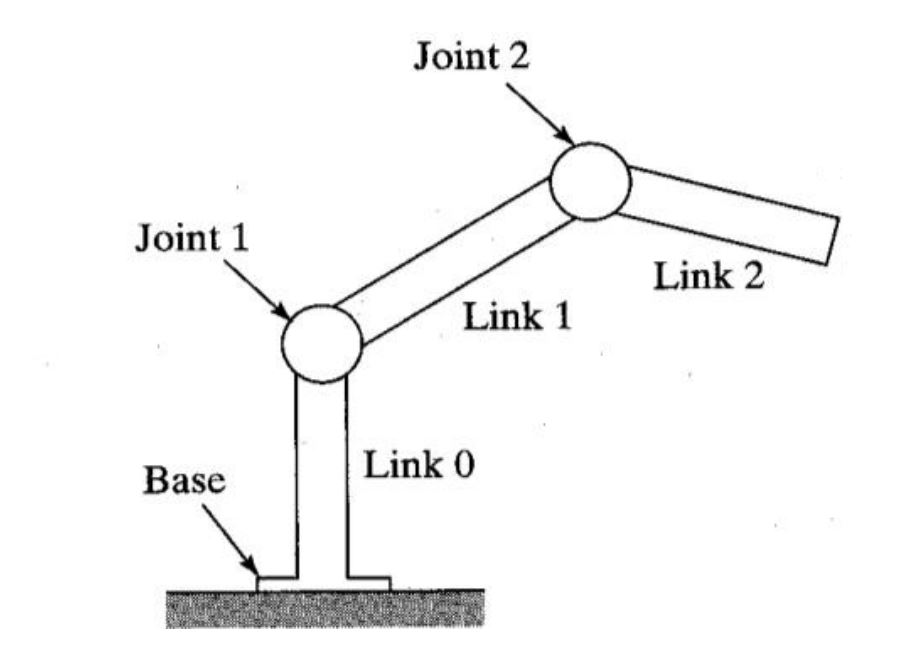
\includegraphics[width=9.2cm, height=6.5cm]{discrete manipulator.JPG}
    \caption{Mechanical components of discrete manipulator}
\end{figure}
\\ \\
Multiple DoF or highly maneuverable manipulators have given rise to a wide variety of designs. The most common design makes use of a backbone like structure that is moved by cable sets. Due to the fact that there are many more actuatable DoFs in the intended workspace, this is frequently referred to as a hyperredundant manipulator. Robinson and Davies [1] created three groups for potential various designs due to the broad design options. First class named as discrete robots that define conventional manipulators, as previously introduced. It enters the second classification, known as serpentine robots, as the manipulator's redundancy/maneuvrability over discrete manipulators grows by increasing the number of discrete joints. Hyperredundant manipulators are included in this classification. As opposed to the first two classifications of robots, the continuum robots categorization does not include split joints or rigid joints as you can see the differences in Figure 3.2. Instead, like the biological body and tentacles, the manipulator is constantly bent throughout its length. The higher DoF that improves the maneuverability of hyper-redundant and continuum robots has the unfavorable effect of making the kinematics of these manipulators more complex.
\newpage
\begin{figure}[h!]
    \centering
    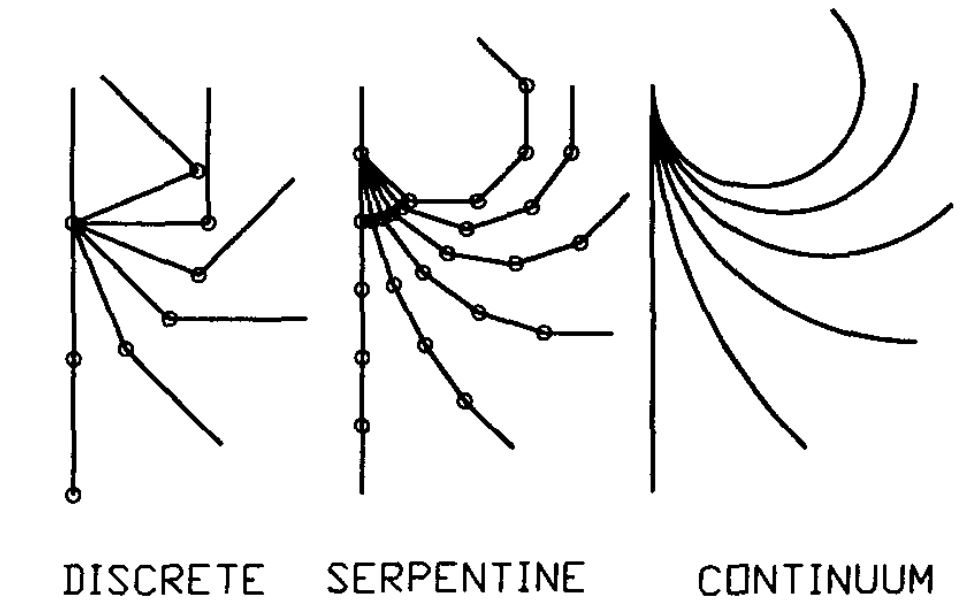
\includegraphics[width=9.7cm, height=6.1cm]{differences.JPG}
    \caption{Class of manipulators [2]}
\end{figure}
\noindent In addition to continuum robots, soft robots must also be defined. The goal of soft robotics is to create robots that can adapt to their environments by having flexible bodies and flexible electronics. Hard robotics also includes the discrete style robots we previously mentioned. According to DoF and material type, [6] classified hard and soft robots, as shown in Figure 3.3.

\begin{figure}[h!]
    \centering
    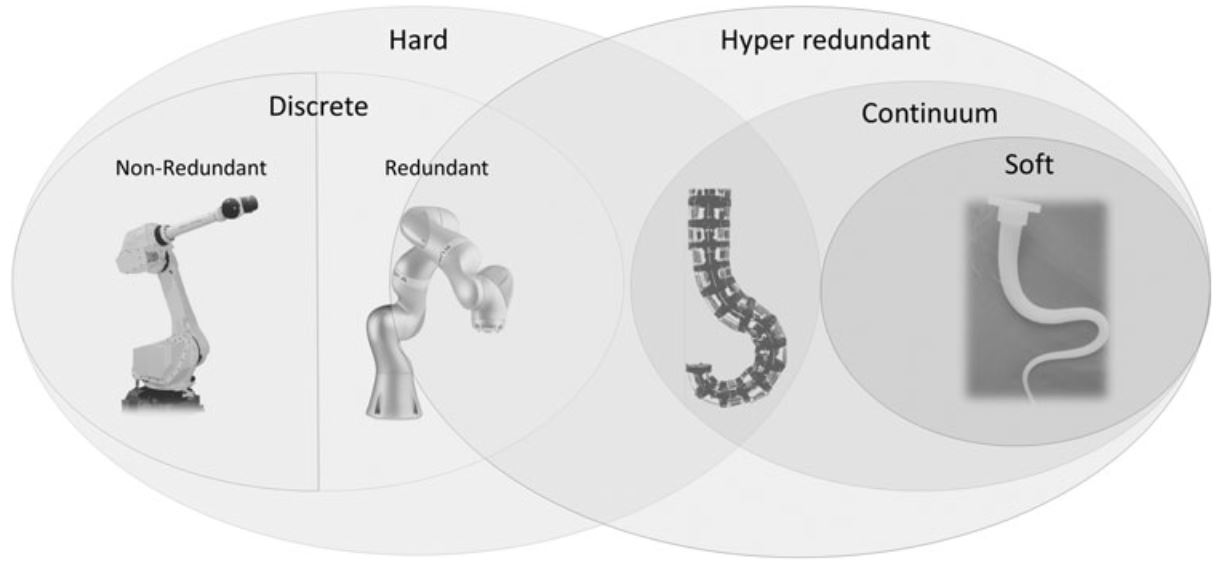
\includegraphics[width=12.3cm, height=5.7cm]{classification.JPG}
    \caption{Classification of manipulators based on materials and DoF}
\end{figure}

\subsubsection{Characteristics of hard and soft robots}
\begin{itemize}
    \item Dexterous motion is made possible by distinct mechanisms in conventional hard robots and soft robots. Soft robots can deform in different places with theoretically infinitely many DoF. This results in a hyper-redundant configuration space, where the robot tip can reach any place in the three-dimensional workspace using any of an endless number of robot configurations or shapes.
    \item Soft robots, as opposed to hard hyper-redundant robots, have the added benefit of producing less resistance to compressive forces, allowing them to adjust to obstacles. As a result, they can safely transport delicate and sensitive payloads.
    \item The actuators of a soft robot determine its limited, controllable DoF. Every joint on rigid-linked robots has an actuator, usually an electric motor. Soft robot actuators are often spread throughout the structure and integrated into it. Actuators frequently make up the majority of the structure. Many conventional hard actuators, such as electric motors, cannot be used in soft robots because of this dual actuator/structure functionality. The actuation method, strain, actuator size, shape, and placement within the structure all contribute to the deformation that results from an actuator being activated. Soft robots belong to a group of systems known as "underactuated" systems because, in contrast to hard robots, they do not have an actuator for every DoF.The actuators may have an impact on some DoF, however many DoF are not controlled.
    \item It can be difficult to sense and control a soft robot's shape. It is challenging to estimate their form and tip position precisely because their structure is continuous. It can be difficult to decide what to measure and how to use the measurements to manage mobility. Hard robots use high-resolution encoders to measure each joint's position. Assuming a rigid robot, the forward kinematics can properly predict the shape and tip location of the robot by processing the joint positions. The joint positions that yield the desired tip position can also be found via inverse kinematics. The required positions derived from the inverse kinematics are compared to the joint positions obtained by the encoders, and the actuators subsequently servo the errors to zero. The joints are forced to accurately track their target locations by the servo action, which is normally fairly rapid.
    \item Soft robots behave differently from their hard counterparts when interacting with the world. The world places loads on the structure through touch or distributed loading (such as gravity). When a rigid-linked robot is loaded, the soft joints move while the rigid links stay in place. The controller can either make a loading adjustment or recognize that the robot has made touch with its environment once the encoders measure the position change. Both the form and the position of the tip may be precisely determined. A soft robot experiences continual deformation brought on by gravity and contact loading that may not be seen or observable by the limited sensors or actuators, respectively.
    \newpage
    \item The mobility of soft robots depends heavily on contact and conformity to the surroundings. Soft robot arms, for instance, manipulate objects with their entire arm to grip and handle objects of various sizes. A strong grip and a high-friction contact allow the arm to raise the object after it is wrapped around it. With a specific end effector that is often created for a particular size and type of object, hard robot arms grasp and handle objects. With a significant amount of their structure constantly in contact with the ground, soft robots may move around by adopting a variety of gaits. Hard robots may move by contacting the ground with their separate legs, tracks, and wheels.
\end{itemize}
You can see Figure 3.4 for a summary of the comparison of soft and hard robots.
\begin{figure}[h]
    \centering
    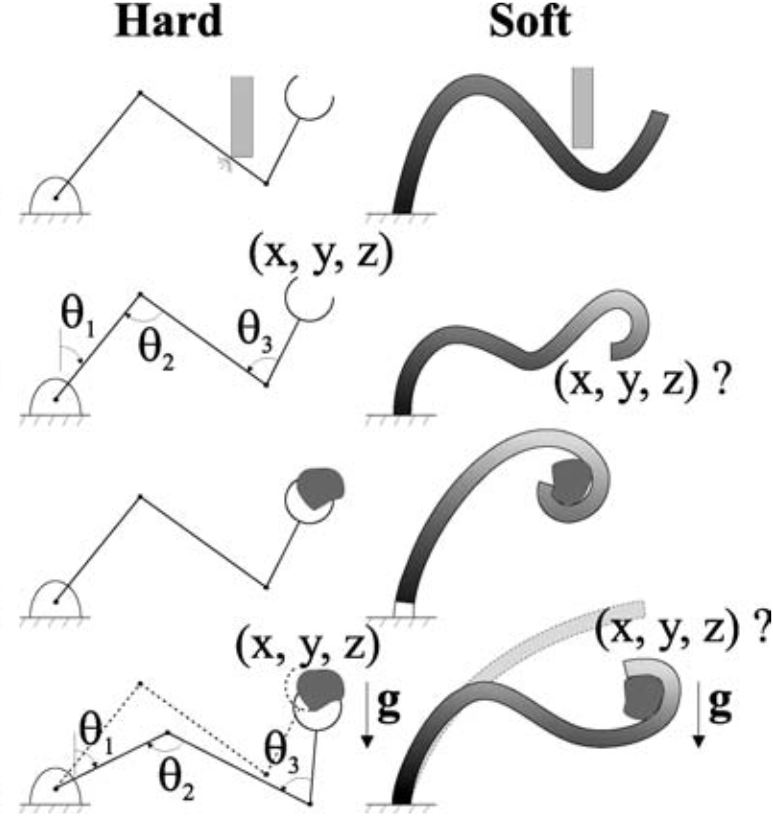
\includegraphics[width=9.3cm, height=8.4cm]{hardvssoft.JPG}
    \caption{Capabilities of soft and hard robots [7]}
\end{figure}
\\ \\
Figure 3.5 illustrates the deformation of a soft robot arm when gravitational loading and actuation are coupled. If the connections are sufficiently rigid and the stress is sufficiently low, hard robots can servo the arm to any shape. A moment or a torque is frequently applied at the tip of a soft robot arm via its actuators. This tip moment leads the arm to bend upward in a quadratic shape for minor displacements. Self-weight bends the arm downward in a cubic shape in a gravitational field. The tip moment can be changed to raise the tip to the horizontal position, however due to the discrepancy between the quadratic and cubic shapes, the arm will not have a zero shape [8]. Similar to this, it is impossible to distinguish between a distributed load and a point load at the tip if a sensor is used to measure the moment at the base of this soft robot arm. However, these loadings result in drastically diverse arm morphologies.
\begin{figure}[h]
    \centering
    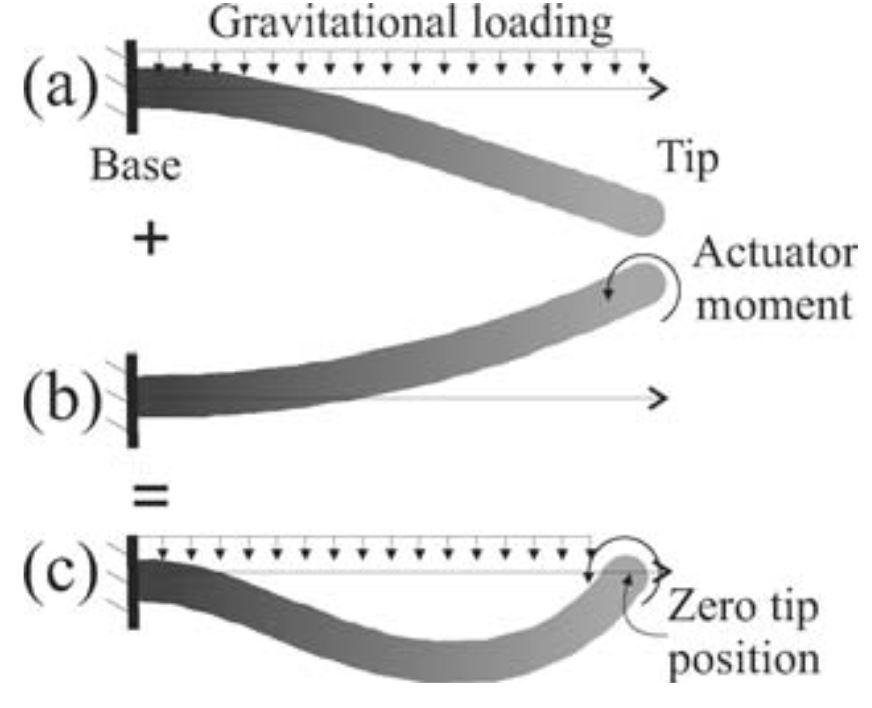
\includegraphics[width=8.7cm, height=7.1cm]{grav.JPG}
    \caption{Gravitational loading on a soft robot manipulator [7]}
\end{figure}
\\ \\ 
Generally, the structure of the continuum robot employed for manipulation is categorized as a single or multisegment [9]. In order to improve functioning, many discs are inserted as a backbone for these robots in order to imitate a continuous structure. The most typical examples of multidisc biomodels with single or multiple segments that consist of a structured alignment of discs are continuum models, which were inspired by the spines of mammals and snakes. You can see several single and multi segment continuum robots in Figure 3.6.
\newpage
\begin{figure}[h]
    \centering
    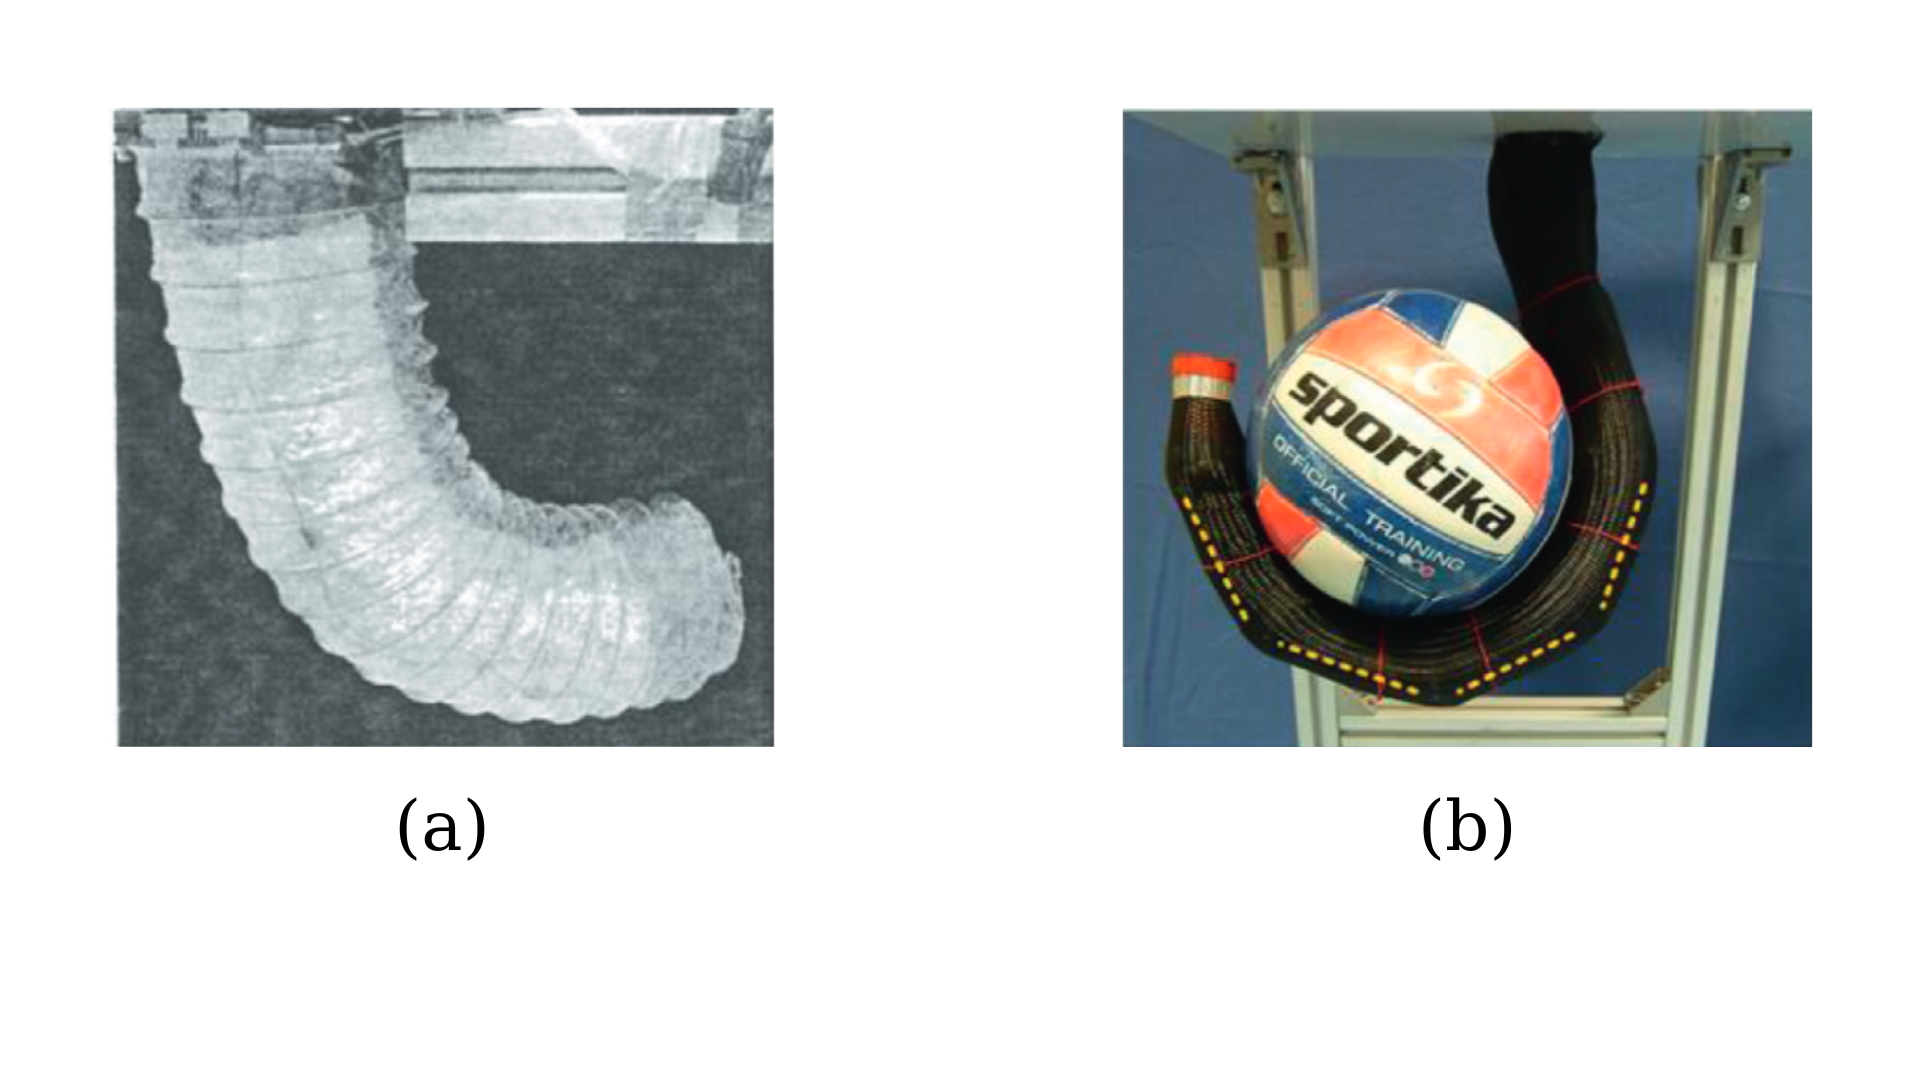
\includegraphics[width=14.25cm, height=7cm]{single-multi.png}
    \caption{Single-segmented (a) and multi-segmented (b) continuum robot [10]}
\end{figure}

\subsection{Applications}
We can see continuum robots in many areas. In this section of the thesis, we will see the application areas of continuum robots.

\subsubsection{Inspection}
Due to structural restrictions, a typical auxiliary inspection system cannot easily complete this task. The continuum robot is better suited for those complicated situations than the conventional discrete robot because it has a higher length-to-diameter ratio, more freedom, and flexible mobility. [11] created a continuum robot to aid pilots in inspecting fuel tanks, thereby lowering workload and improving maintenance effectiveness.

\subsubsection{Medical}
Because of the limited DoF imposed by their construction and material, conventional rigid robots have limited applications in the medical industry. The continuum robot, which was modeled like snakes, tentacles, and trunks, was able to maneuver through small spaces, move objects in challenging environments, and follow curved trajectories in space. Due to its remarkable dexterity and ability to access intricate parts of the body and execute precise surgery, the continuum robot has a wide range of potential applications in surgery. Researchers have recently made numerous attempts to enhance continuum robot design and actuation techniques. Numerous continuum robots have been used in surgical clinic operations and have shown advantages over traditional rigid-link robots.
\\ \\
Bevel-tipped flexible needles with duty-cycled spinning during insertion to target sites for drug administration inside the brain have been suggested by [12]. A curved path can be created by steering the bevel-tipped needle. In particular, tip-steerable needles are a kind of continuum robot. [12] described a method for evacuating intracerebral hemorrhage utilizing a concentric-tube continuum robot (see Figure 3.7). This particular robot is made up of two tubes: the inner aspiration tube is straight followed by a curved segment for extracting the bleeding from within, and the outer tube is straight for accessing a blood clot within the brain via a direct linear path.
\begin{figure}[h]
    \centering
    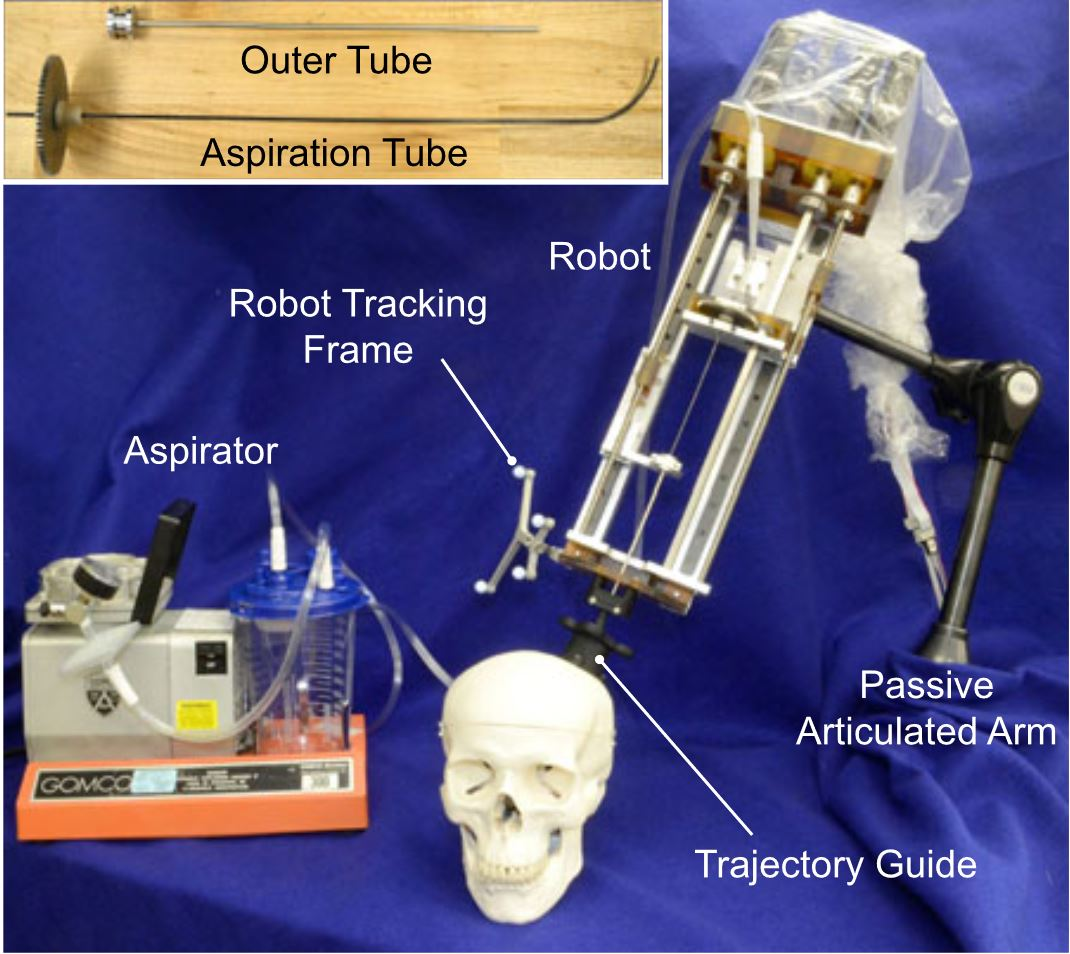
\includegraphics[width=9.3cm, height=8.0cm]{medic1.JPG}
    \caption{Two-tube concentric-tube continuum robot for medical application [12]}
\end{figure}

\noindent As some other examples, Flexible endoscopes are used in clinical practice to perform endoscopic sinus surgery [13] and [14] demonstrated a telerobotic system for throat surgery that was clinically driven by the demand for enhanced 3-D vision and distal instrument movement.

\subsubsection{Antennas}
In wireless applications for the Internet of Things (IoT), search and rescue, communications, and power distribution, antennas are essential parts. These devices are made of metal structures that transform time-varying current into electromagnetic radiation, and the physical makeup of the metal has a significant impact on how they behave. It is possible to drastically regulate and tune an antenna's performance by bending, twisting, and altering its geometry. [15] show the design and analysis of a reconfigurable and deployable antenna that creates the 3D antenna structure using a growing continuum robot (Figure 3.8).
\begin{figure}[h]
    \centering
    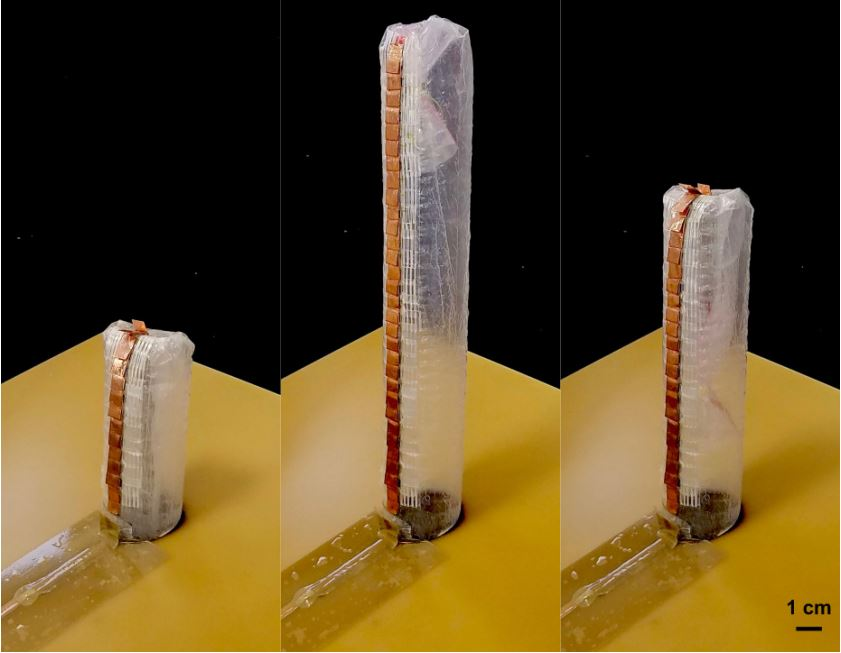
\includegraphics[width=8.4cm, height=6.5cm]{ant.JPG}
    \caption{Continuum robot for antenna application [15]}
\end{figure}

\subsubsection{Hazardous places}
Robots that operate in a continuum can perform tasks in perilous and dangerous conditions. For instance, a quadruped robot with continuum limbs has been constructed. It can traverse challenging barriers by moving through the gaits of walking, crawling, trotting, and complete arm gripping [16].
\begin{figure}[h]
    \centering
    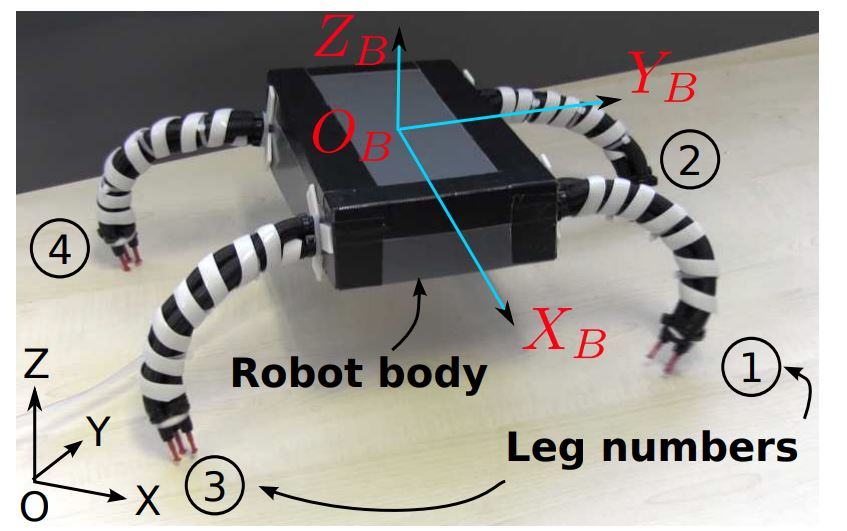
\includegraphics[width=8.4cm, height=5.3cm]{hazardous.JPG}
    \caption{Locomotion with Continuum Limbs [16]}
\end{figure}

\subsubsection{Space}
Tendril, a continuum manipulator created by NASA, can extend into crevasses and beneath thermal blankets to reach places that are otherwise inaccessible using standard technology [106]. Besides, [107] propose a novel mechanical scaly layer-jamming design for space applications that enhances the functionality of earlier continuum robots.
\subsubsection{Subsea}
While the FLAPS project generated propulsion systems that mimicked fish swimming, the AMADEUS project created a dexterous underwater robot for grasping and manipulation activities [108]. A kinematic and dynamic model for an underwater robotic manipulator that is inspired by Octopus vulgaris is presented in [109]. The model is then experimentally confirmed before being applied to a prototype arm that was inspired by a living octopus.

\subsection{Kinematics Modelling}
Models of robot shape and motion are necessary for the use of continuum robotics in actual applications. Such models, which have a greater number of flexible links than conventional robots, must necessarily be more sophisticated. This section's goal is to give a general overview of continuum robot model design.
\\ \\
Numerous continuum robot designs have been introduced in recent years. Analytical models are needed in order to develop, analyze, and control such robotic manipulators. They make it possible to determine the robot's final distorted shape given particular actuation inputs. The actuator space, that describes the actuation of the robot's backbone, is mapped to a configuration space, which parameterizes the robot's shape. The resultant position and orientation of the shape in task space are then transferred by the configuration space parameters. The mapping between actuation and configuration space can also incorporate a variety of progressively more complicated assumptions about the kinematics of the robot's backbone. As a result, current kinematic models frequently make compromises between accuracy and calculation speed depending on the envisioned application. They are also frequently adapted to a certain robot design. For instance, continuum robot design involves models that accurately describe robot behavior without imposing strict temporal constraints on computing. Since sensor feedback can correct for model errors, robot control is less accurate but still requires quick calculation.
\\ \\
There are several kinematic frameworks that can be used in Continuum robot modelling. [17] applied some of these models (Figure 3.10). We chose the constant curvature model as the kinematic model for its convenience. We'll talk about constant curvature for the rest of the section.
\begin{figure}[h]
    \centering
    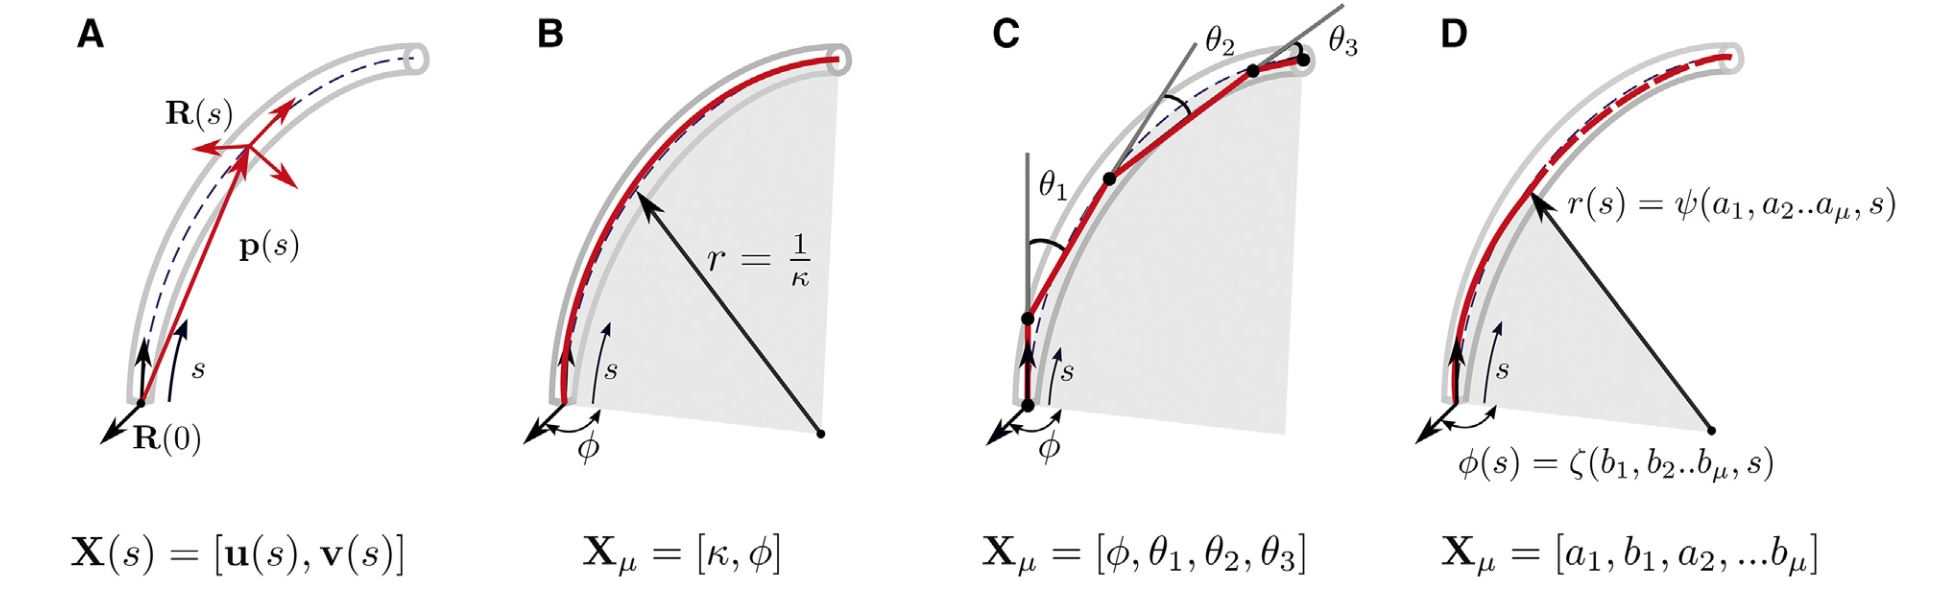
\includegraphics[width=16.25cm, height=5.0cm]{models.JPG}
    \caption{(A) Variable curvature representation (B) Constant curvature representation (C) Pseudo-rigid body  (D) modal approach [17]}
\end{figure}

\subsubsection{Constant Curvature Representation}
Due of the simplifications it allows in kinematic modeling, constant curvature has frequently been seen as a desirable attribute in continuum robots. Robots with constant curvature can be thought of as being made up of an infinite number of curved linkages, whereas elastic structures with variable curvature are defined by integrated functions. A limited number of arc parameters that can be transformed into analytical frame transformations characterize these links.
\\ \\ 
Figure 3.11 illustrates how decomposing kinematics into two mappings is made possible by the constant curvature assumption. 
\newpage
\begin{figure}[h]
    \centering
    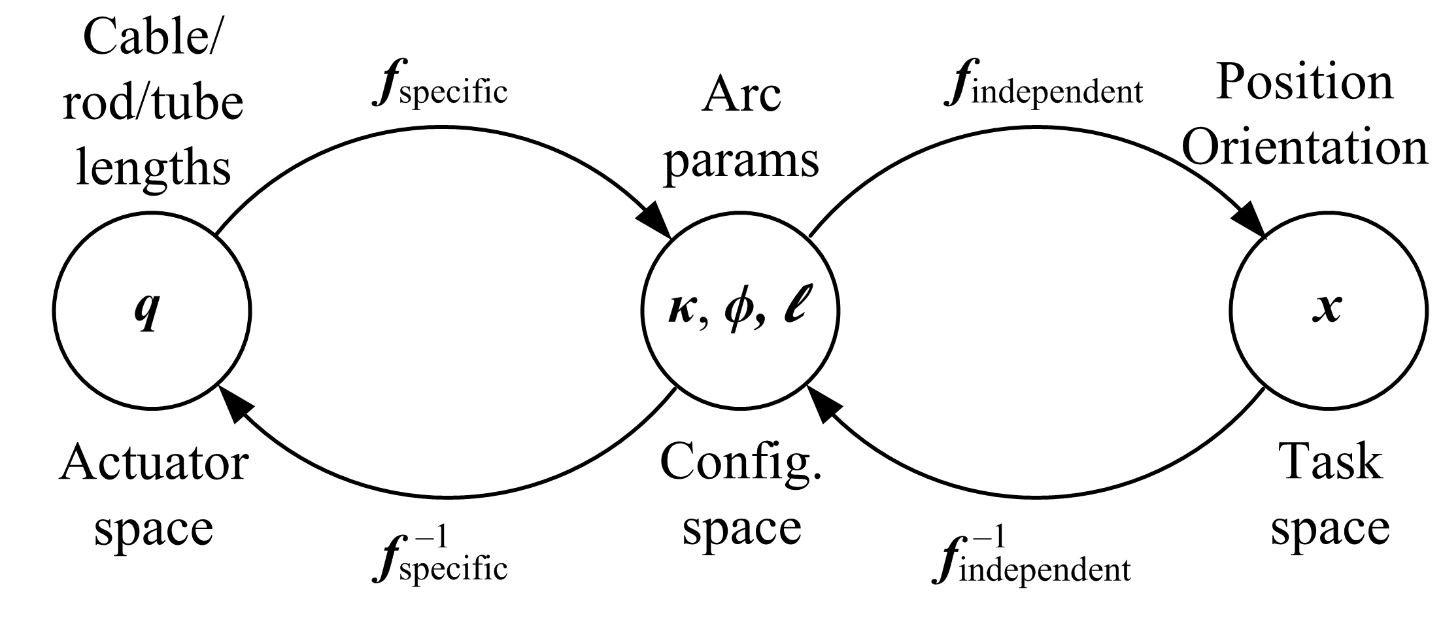
\includegraphics[width=10.0cm, height=4.0cm]{map.JPG}
    \caption{Mappings with kinematics of constant curvature representation}
\end{figure}

\noindent A constant-curvature arc is described by parameters that are transferred from actuator space to configuration space. The second one is from this configuration space to task space, and it consists of a space curve that represents location and orientation along the backbone. Figure 3.12 illustrates how the curvature, angle of the plane containing the arc, and arc length make up the arc parameters, which determine the configuration space of the robot. Finally, the task space is the position and the orientation of the robot.
\begin{figure}[h]
    \centering
    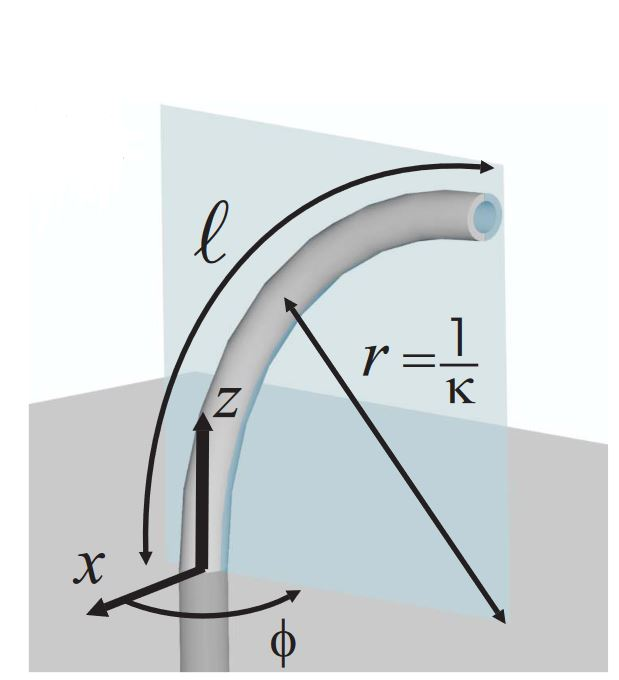
\includegraphics[width=6.2cm, height=6.8cm]{arc.JPG}
    \caption{Arc parameters which describe a circular arc [18]}
\end{figure}

\noindent Because actuators in each distinct robot design have a different impact on arc parameters, the mapping $f_{specific}$ from actuator space, which is represented as $q$, to the configuration space of arc parameters, which is represented as $(K,\phi,l)$, is robot-specific. This mapping from actuator variables (pressure, length, etc.) to circular sections described by arc parameters in configuration space is made possible, in particular, by taking into account the forces and moments applied by actuators in conjunction with suitable approximations. As a result of being applicable to any systems that can be approximated as constant curvature arcs, the mapping $f_{independent}$ from arc parameters to position x along the backbone is robot-independent. This transformation from arc parameters to a space curve in task space is purely kinematic [18].

\subsection{Control}
With the increasing interest in soft robots, the development of suitable controllers has become necessary. Fundamentally different from traditional rigid robots, a unified framework for the design, analysis, and control of these high-dimensional robots has recently begun to be developed. Evaluation of various control strategies will be made in this section. 
\\ \\
For a better understanding of this part of the thesis, it is necessary to look carefully at Figure 3.13. This figure is taken from [6] provides different levels of mapping involved in the control of a continuum/soft manipulator. In addition, a more simplified mapping is discussed in Figure 3.11.
\begin{figure}[h]
    \centering
    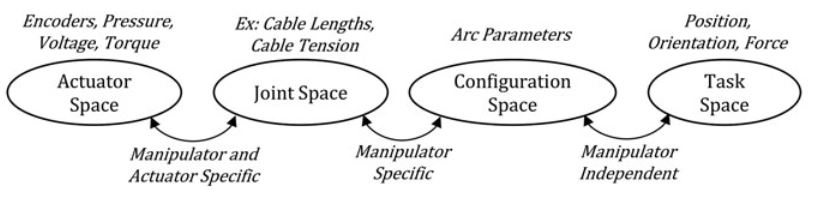
\includegraphics[width=14.0cm, height=3.63cm]{map2.JPG}
    \caption{Operating spaces of a continuum robot [6]}
\end{figure}

\noindent Controllers can be divided into 4 classes as model-based static, model-based dynamic, model-free static and model-free dynamic controllers. The methods used for each controller class will be briefly mentioned as sub-sections. 

\subsubsection{Model-Based Static Controllers}
Soft continuum robots are a difficult robot category to model due to their high number of DoFs (theoretically infinite). However, with various assumptions, the exact configuration of soft continuum robots can be described by a low-dimensional state space representation. The simplest and most popular kinematic/steady-state model, known as the constant curvature (CC) approximation, implies that the configuration space of a three- or two-dimensional (planar or spatial) continuum/soft module can be parameterized by variables [36]. It ignores the majority of the dynamics of the manipulator by condensing an infinite dimensional structure to simply 3D or even 2D. 
\\ \\ 
In addition to this simple modeling strategy, a more intricate modeling strategy was implemented using beam theory [53] and Cosserat rod theory [54]. To get the desired actuator or configuration space variables, a kinematic model must first be built and then the kinematics must be inverted. This can be accomplished by direct inversion [57] or optimization [58] with differential inverse kinematics (IK) [55,56], both of which have been extensively researched for solid manipulators. Additionally, a low-level controller typically uses a straightforward linear closed-loop controller to monitor the actuator/junction area. Additionally, the presence of friction, hysteresis, or tendon coupling [59, 60], which can deviate from the forward steady-state model, may necessitate the adoption of actuator compensation approaches.
\\ \\ 
The desired joint configuration that decreases the current tracking error is estimated while satisfying the forward kinematic model and cable tension constraints in [58], which formulates the inverse kinematics problem as a constrained nonlinear optimization problem. They gain leverage in terms of greater accuracy and robustness to model uncertainties by representing the kinematics at the velocity level. However, they would first need to solve a high-level path planner like that in Figure 3.14. The direct task space controller's drawbacks include instability and delayed convergence.
\begin{figure}[h]
    \centering
    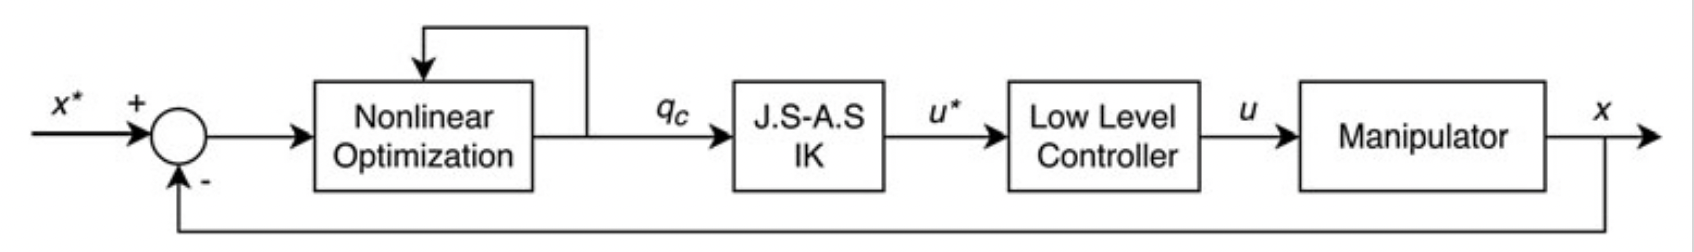
\includegraphics[width=15.3cm, height=2.5cm]{cont1.png}
    \caption{A closed-loop task space controller [6]}
\end{figure}

\noindent It is proposed by [61] that a configuration space controller that asymptotically tracks a stationary configuration goal using both internal and exterior sensory input regarding joint variables and configuration.
\newpage
\noindent Similar to this, two closed loop controllers in the joint space of Figure 3.15 and the task space of Figure 3.16 were compared in [62]. A direct closed-loop task space controller has the benefit of allowing for asymptotic convergence of the error even in the presence of model uncertainties.
\begin{figure}[h]
    \centering
    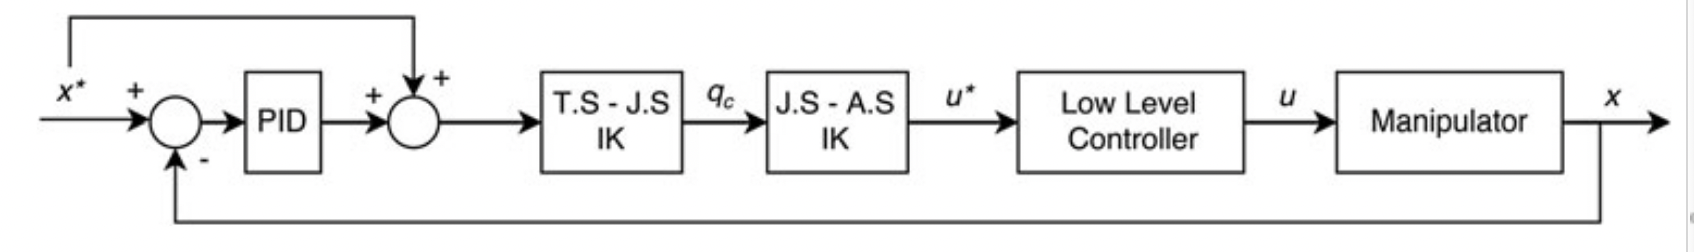
\includegraphics[width=15.3cm, height=2.8cm]{cont2.png}
    \caption{A closed-loop task space controller with PID [6]}
\end{figure}

\noindent It was shown in [63] that an estimate of the external generalized forces can be formed by knowing the configuration space variables and the current internal actuation forces. A configuration space controller for lowering tip forces for surgical purposes was proposed using the estimated external force and the compliance matrix. 
\begin{figure}[h]
    \centering
    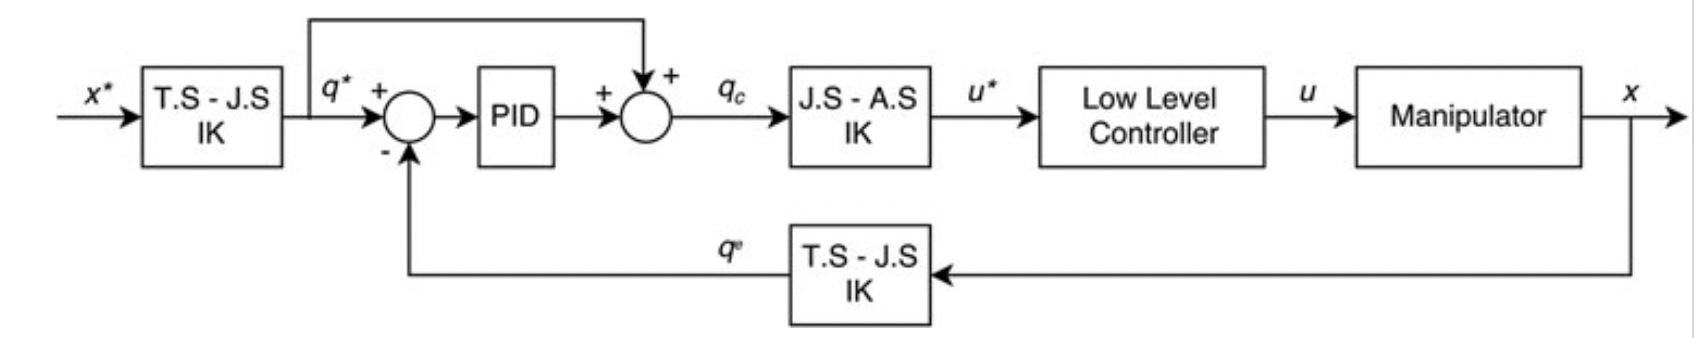
\includegraphics[width=15.3cm, height=3.0cm]{cont3.png}
    \caption{A task space controller implemented in the joint space. [6]}
\end{figure}

\noindent Figure 3.17 depicts the realization of a hybrid position/force controller in the configuration space in [64] which is extension of [63]. Besides, [65] achieved hybrid position/force control without the use of force sensors.
\newpage
\begin{figure}[h]
    \centering
    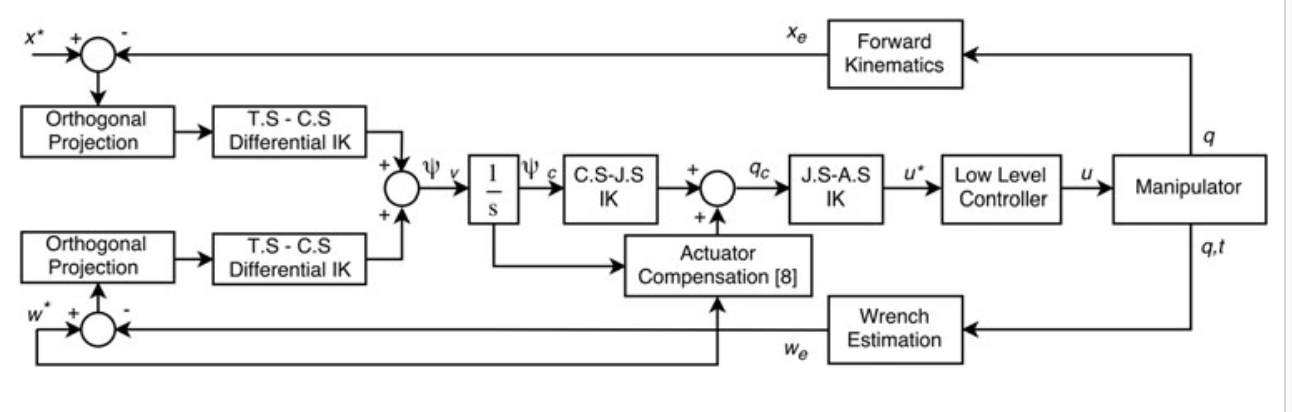
\includegraphics[width=15.0cm, height=6.2cm]{cont4.png}
    \caption{Closed-loop task space control of position and force [6]}
\end{figure}

\noindent The VCC model (variable constant curvature approximation) was suggested for visual servo control of a two-dimensional (2D) image feature point in 3D space using a cable-driven soft conical manipulator in [66]. A differential kinematic-based controller with the control goal of decreasing the feature point tracking error was proposed. It is similar to the one in [67]. % Also described was an adaptive depth estimation algorithm.
\\ \\ 
Currently, the most popular and extensively researched method for controlling soft continuum robots is model-based static control. 
% Since more complex models are computationally costly and design-specific, the majority of model-based controllers rely on the CC approximation, which we also used in this thesis. Despite this, the CC model is still one of the most effective and simple techniques for static control of uniform, low-mass manipulators because to the validation of the model for a fully soft robot and its extensive application for control of different continuum or soft robots. A joint space controller or closed-loop configuration space controller would deliver more reliable and quick controllers, but they cannot ensure error convergence (unless there is a perfect forward model available). The most accurate system might theoretically be a closed-loop task space controller. Tendon-driven systems are more challenging to simulate in terms of actuation, whereas pneumatic manipulators would require more sensors.

\subsubsection{Model-Free Static Controllers}
Soft Continuum robot control using model-free methods is a relatively young field with many potential applications. The same cannot be stated for continuum manipulators, despite the fact that these data-dependent methods have been employed successfully in the field of rigid manipulators [68], despite the fact that model-free approaches ought to perform better in this situation.
\\ \\
It was first suggested in [69] to use a model-free methodology for developing a static controller. The method involved utilizing a neural network to directly learn the inverse statics of a soft robot that was non-redundant (in terms of actuator space and task space). For a cable-driven soft manipulator [71], an experimental validation of the same methodology was conducted and compared with an inverse kinematics model generated from a numerically precise model in [70]. 
\\ \\
It's interesting to note that the straightforward neural network-based strategy outperformed the computational complicated analytical technique by a wide margin. The final controller resembles the illustration in Figure 3.18 but does not include the feedback component. 
\begin{figure}[h]
    \centering
    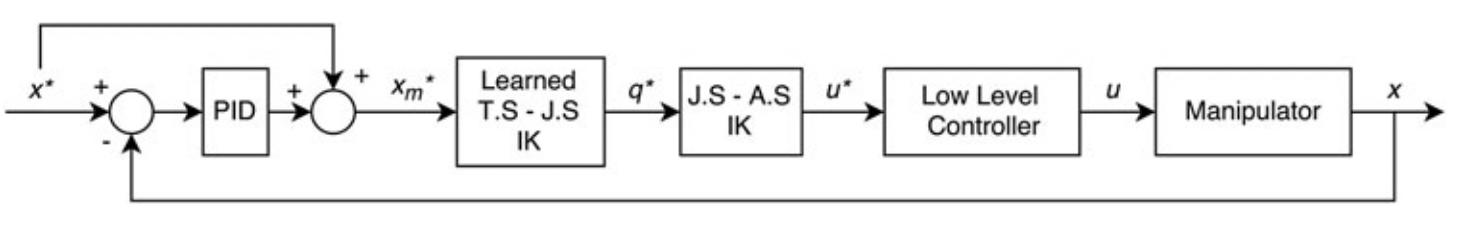
\includegraphics[width=15.3cm, height=2.8cm]{cont5.png}
    \caption{A general model-free closed-loop task space controller [6]}
\end{figure}

\noindent In [72], an effective exploration technique for producing samples for IK learning was put out. Also, For closed-loop task space control of continuum robots, a very reliable, accurate, and general method was put out in [73] as shown in Figure 3.19. The study suggests an optimal control technique based on empirically estimating the kinematic Jacobian matrix while each actuator is being moved incrementally online. The cables are kept taut and the control effort is reduced by optimization. The authors refer to the method as a "model-less" methodology because there is no internal model employed for control. The relatively low control frequency is a practical concern despite the fact that this approach resolves many control issues with continuum robots, even permitting manipulation in an unstructured environment.
\\ \\
To learn deterministic stationary policies for a soft robot arm module,  [75] maximize various objectives within a RL framework. Although it operates in high dimensions, it is susceptible to perturbations from the outside world. In [76], a move toward fuzzy logic-based controllers was made. The goal was to construct numerical estimates of the kinematic Jacobian using local approximations and interpolation functions based on prior knowledge. This enables speedier computation, however it's unclear how this method is superior to data-driven ML techniques.
\newpage
\begin{figure}[h]
    \centering
    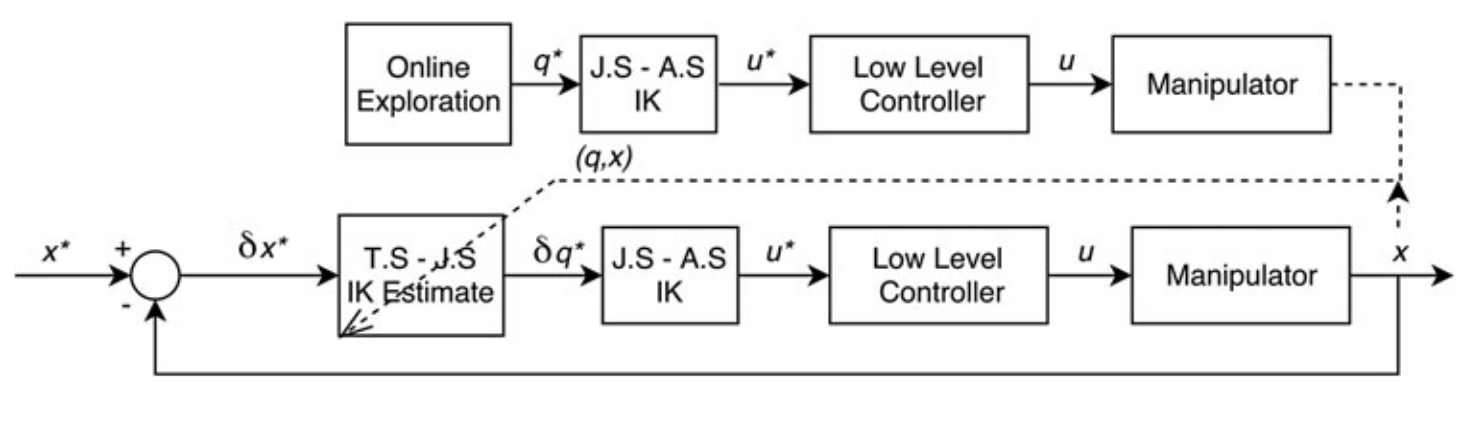
\includegraphics[width=15.0cm, height=4.5cm]{cont6.png}
    \caption{Model-free control strategy. [6]}
\end{figure}

\noindent Transfer learning has also been attempted, but it has only involved simulation [74]. They created an algorithm to move the reaching abilities from a CC soft continuum robot to a non-CC octopus arm in simulation. The goal is to create dynamic motion primitives by combining weighted Gaussian functions that represent the data's joint distribution. This makes it resistant to environmental disturbances when paired with a statistical regression approach. This strategy appears promising, but additional testing is needed to show how effective it is. 
\\ \\
The fact that model-free approaches are independent of the shape of the manipulator and do not require defining the parameters of the configuration space or joint space is one of their main advantages. Due to the abundance of sample data and sensory noise, arbitrary complex kinematic models can be created. For systems that are highly nonlinear, nonuniform, subject to gravity, or operate in environments with little structure, model-free approaches have likely performed better. Model-based controllers are still superior in terms of accuracy and dependability for well-behaved small manipulators operating in well-known environments. Furthermore, stability analysis and convergence proofs are challenging to establish due to their black box nature. There is little to no dynamic coupling between sections, according to static/kinematic controllers. As was mentioned at the outset, static/kinematic controllers rely on the steady-state assumption, which makes it difficult for soft manipulators to move accurately and quickly. Therefore, for quicker, dexterous, efficient, smoother tracking as well as in circumstances where coupling effects cannot be disregarded, controllers that take into account the dynamic behavior of these manipulators are crucial.
\\ \\
The creation of nonstatic controllers that take into account the entire dynamics of the entire manipulator is likely the most difficult aspect of controlling continuum/soft robots. The formulation of the kinematic model and an associated dynamic formulation are necessary for the development of dynamic controllers. An imprecise dynamic formulation based on kinematic models, which are challenging to develop themselves, exacerbates the model uncertainties. 
\\ \\
Within the scope of this thesis, model-based and model-free dynamic controllers will not be discussed, since the dynamic design of the continuum robotic system is not done, and it is not used in RL control.

\section{Reinforcement Learning}
Today, the majority of AI studies focus on ML. Modeling of problems in ML is basically examined in three classes as supervised learning, unsupervised learning and RL as shown in Figure 3.20.
\begin{figure}[h]
    \centering
    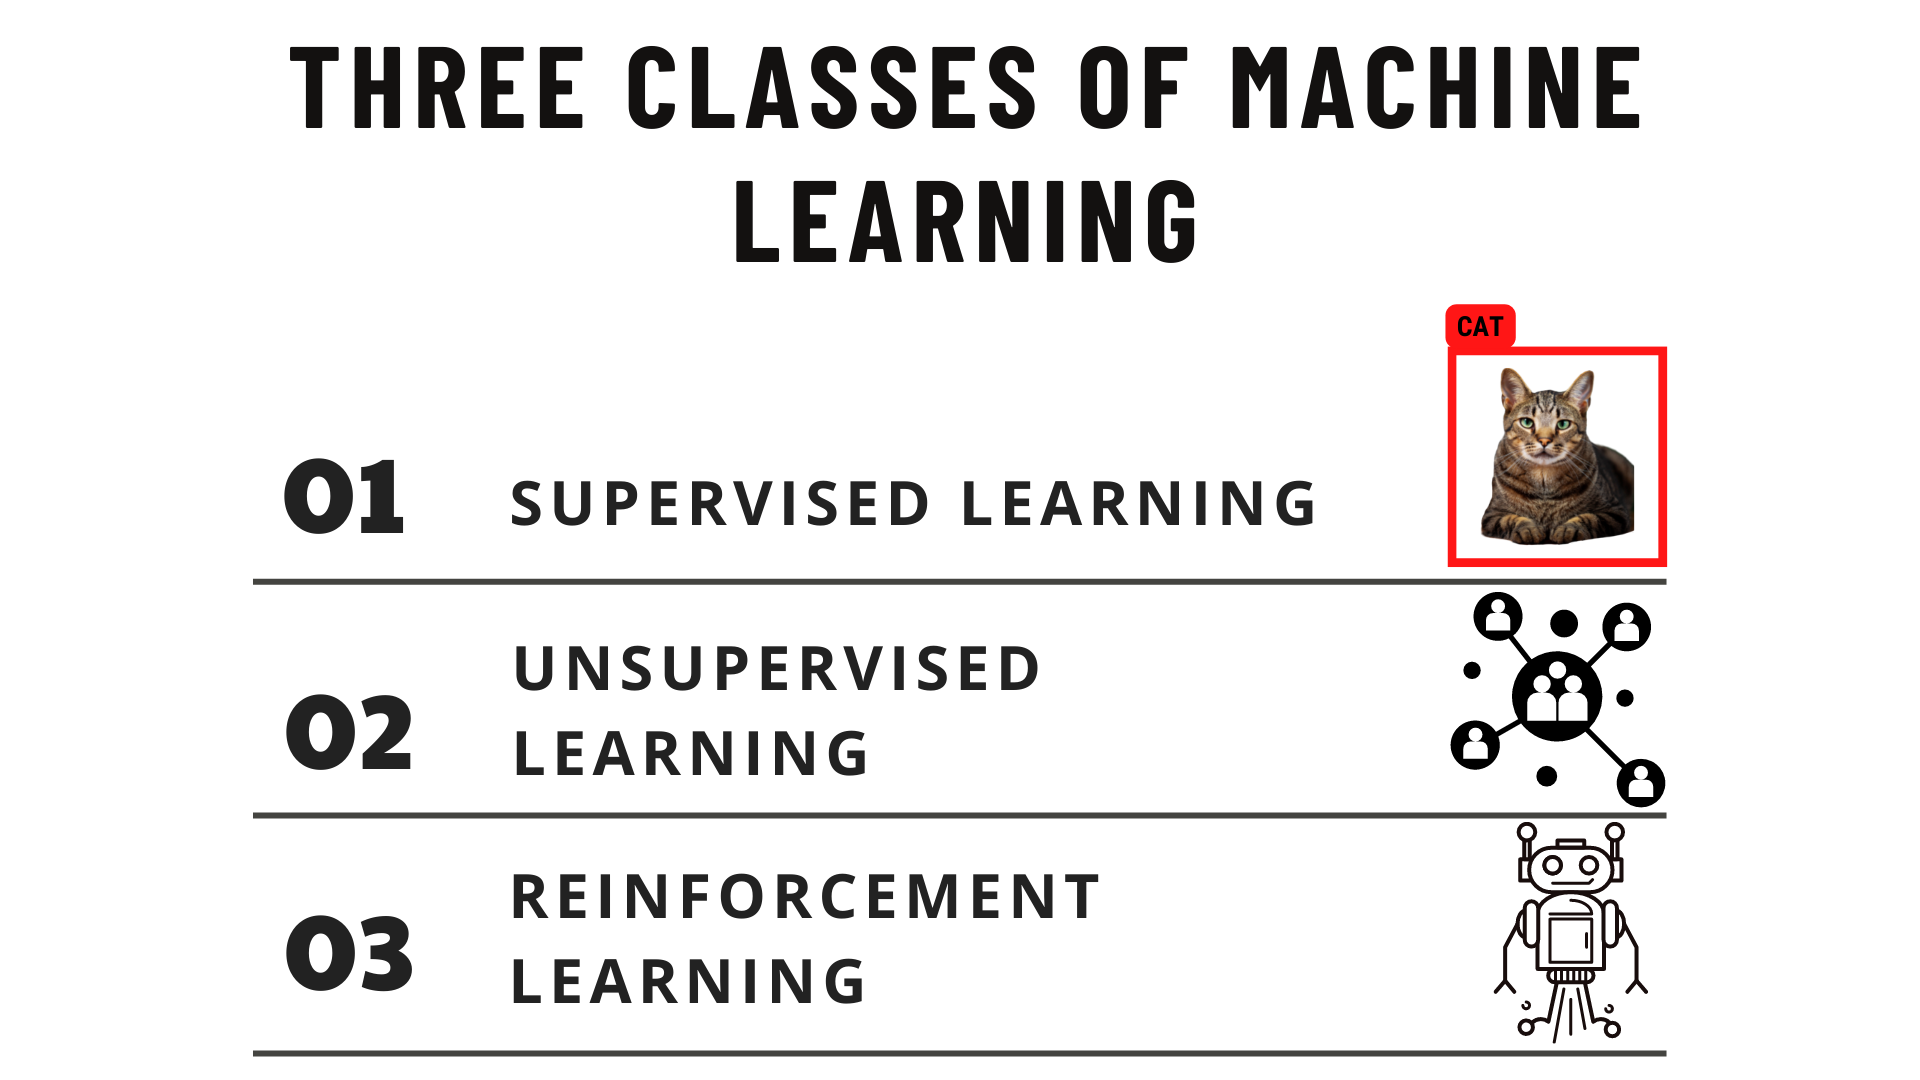
\includegraphics[width=14.0cm, height=8.0cm]{ML.png}
    \caption{Subfields of Machine Learning}
\end{figure}

\noindent ML methods are data-driven and produce solutions to real-life problems. In the supervised learning concept, which is a ML paradigm, there is input and output data for the ML algorithm. Output data can be categorical or numerical data. The problems that supervised learning tries to solve are basically transformed into classification and regression problems. With the solution of the classification problem, applications are made in many fields such as pattern recognition, face recognition, fingerprint recognition, license plate recognition, spam mail identification, decision-making, medical diagnosis, weather forecasting. With the solution of the regression problem, there are application areas such as process modeling, time series estimation, control theory, etc. Another ML paradigm is unsupervised learning. This type of problem mainly deals with clustering problems. In the unsupervised learning model, we have input data collected from real life or a process. Without the label data corresponding to our input data, the developed ML models solve many problems such as detecting clusters in the data, anomaly detection, decision-making, pattern extraction, etc. In RL, which is another paradigm, there is no input and output data for our artificial model, it aims to collect rewards for fulfilling the determined goal by interacting with the environment in which our artificial model is located, and to create these collected rewards at the maximum or minimum level. RL was inspired by behavioral psychology and it provides a formal framework for many control issues. The central hypothesis is that, like a biological agent, an artificial agent can learn through interaction with its environment. The artificial agent should be able to optimize some goals that are provided in the form of cumulative rewards using the accumulated experience. In theory, this method can be used to solve any sequential decision problem based on prior experience.
\\ \\
Thanks to these algorithms, many problems are solved with supervised, unsupervised and reinforcement learning. In this thesis, a RL model was developed, and a solution was created with the DDPG Algorithm to control problem of the continuum robot arm, which is stated in chapter 6. Today, RL has achieved many successes in many critical applications such as finance, robotics, aviation, etc. RL solves many problems that optimal control theory cannot [19].

\subsection{Applications}
RL has rapidly grown in popularity for several years after its discovery of the ability to effectively solve difficult sequential decision making problems. It was able to solve a lot of problems before DL and RL came to be. However, with the fusion of RL with DL methods, it both solved more problems and increased the success rate. Deep RL is a mix of the two fields that works better for high dimensional state space themes. Character selection was a formidable design challenge for previous RL systems. However, due to its capacity to learn various levels of abstraction from data, deep RL has had success with complex tasks with less prior knowledge. For example, a deep RL agent can successfully learn from inputs representing hundreds of pixels of visual perception. This makes it possible to simulate some aspects of human problem solving even in higher dimensional space that was previously difficult to imagine.
\\ \\
To reach beyond human levels, from extracting meaning from pixels to playing video games [77], to mastering the game of Go with programs like Alpha Go [78] or beating even the best poker players in the world [79, 80], a number of important experiments using deep RL in games have come. RL and Deep RL are not only used in games, but also in fields such as robotics [81, 82, 83], autonomous vehicles [84], banking [85], smart grids [86] and the energy sector [87], both in industry and academia. 
\\ \\
In this section, where we talk about RL applications, it is impossible not to mention OpenAI [88]. OpenAI is a research company working in the field of AI. The company's mission is to bring the benefit of artificial general intelligence to all of humanity. Here, 3 important applications of the company in the field of RL will be mentioned (Figure 3.21):
\begin{itemize}
    \item OpenAI Five [89]: It is a computer program that plays the video game Dota 2 on a five-on-five basis. In 2019, this program became the first AI system to beat world champions in esports competition.
    \item Emergent Tool Use from Multi-Agent Interaction [90]: In a simulation, characters learn how to use increasingly complex tools while engaging in a straightforward game of hide and seek.
    \item Solving Rubik's Cube with a Robot Hand [91]: Deep RL was trained by the company to solve Rubik's Cube problem using a robot hand that resembles a human hand.
\end{itemize}
\newpage
\begin{figure}[h]
    \centering
    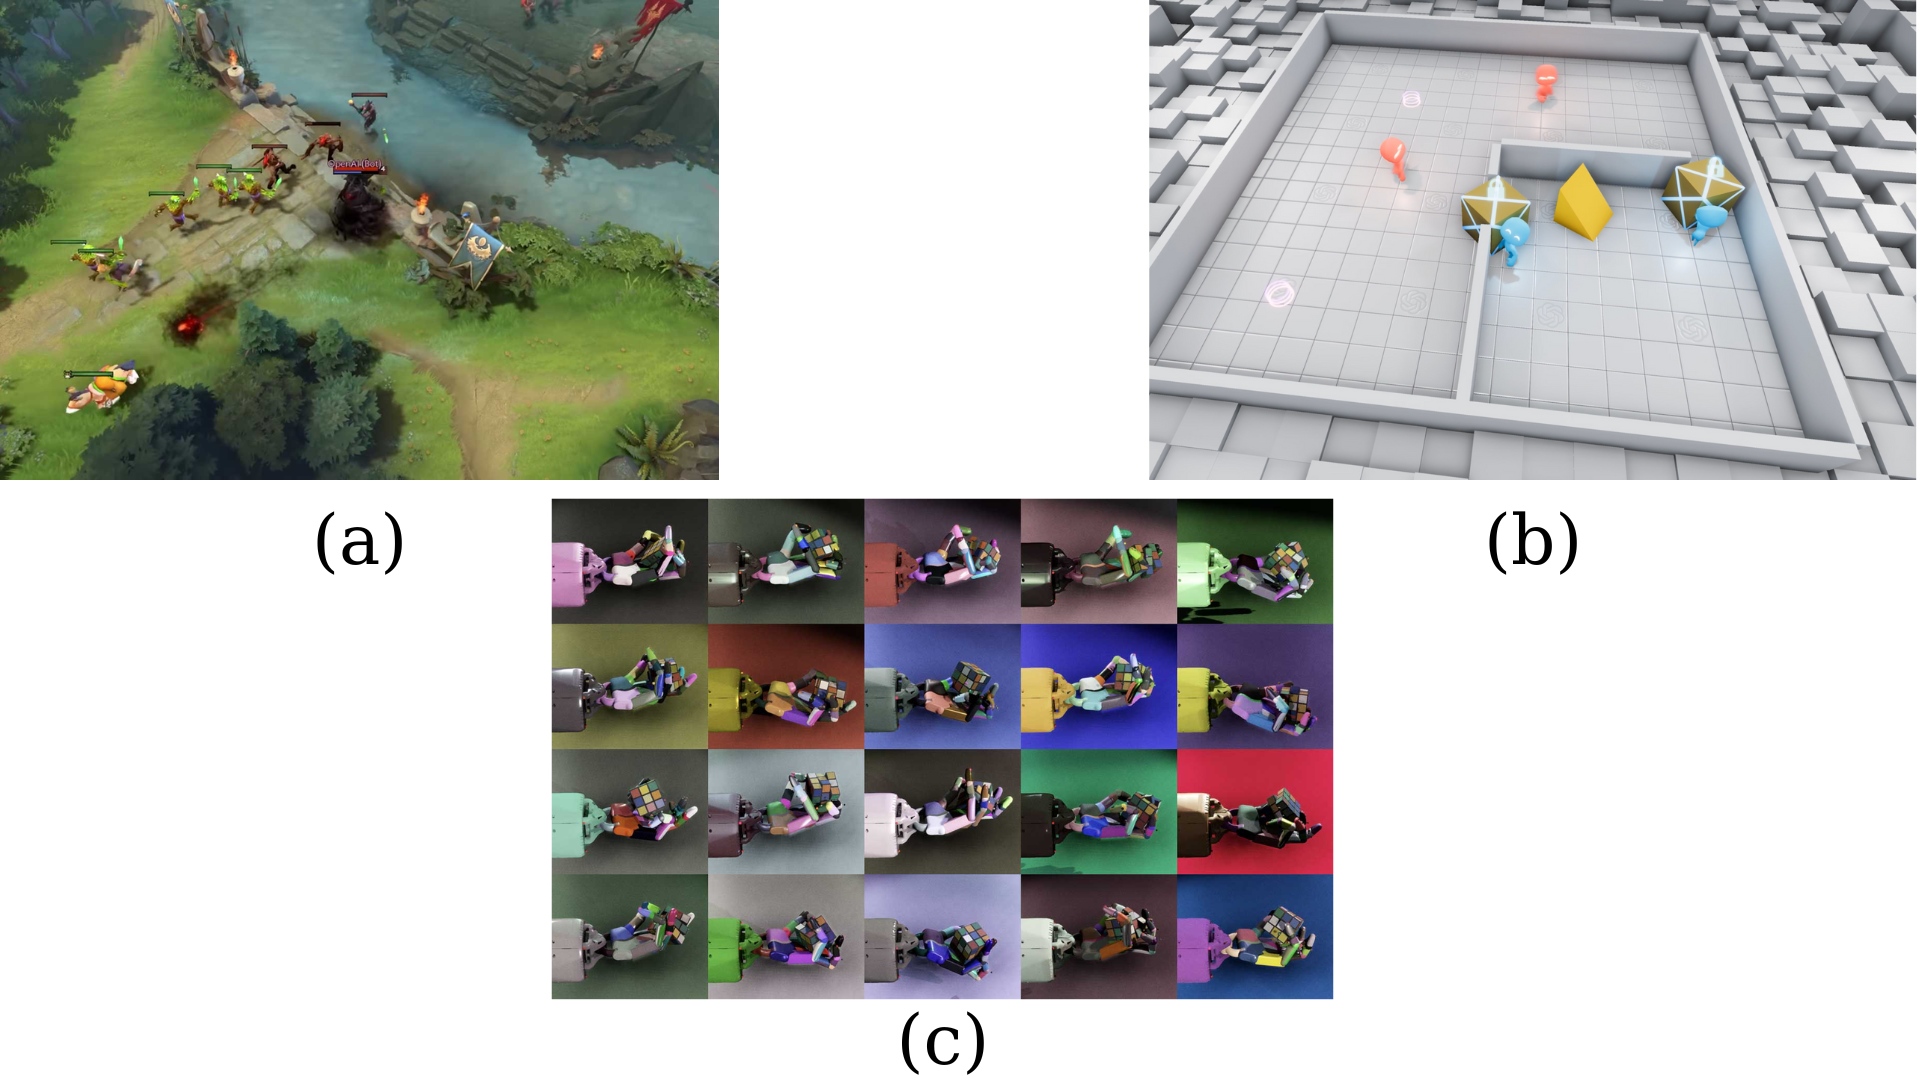
\includegraphics[width=14.0cm, height=8.0cm]{openai.png}
    \caption{Applications from OpenAI company. (a) Dota 2 Game, (b) Multi-Agent Interaction, (c) Rubik's Cube Solving }
\end{figure}

\noindent Since the main purpose of this thesis is the control of a robot with RL method, the next section will focus on the robotic applications of RL.

\subsubsection{Reinforcement Learning in Robotics}
In robotics, any robot can interact with its environment and autonomously determine the best path or behavior through trial and error thanks to RL. In RL, the creator of a control task provides feedback in terms of a scalar objective function that measures the robot's one-step performance rather than explicitly describing the mathematical details of a problem's solution. Figure 3.22 displays several robots created using RL.
\newpage 
\begin{figure}[h]
    \centering
    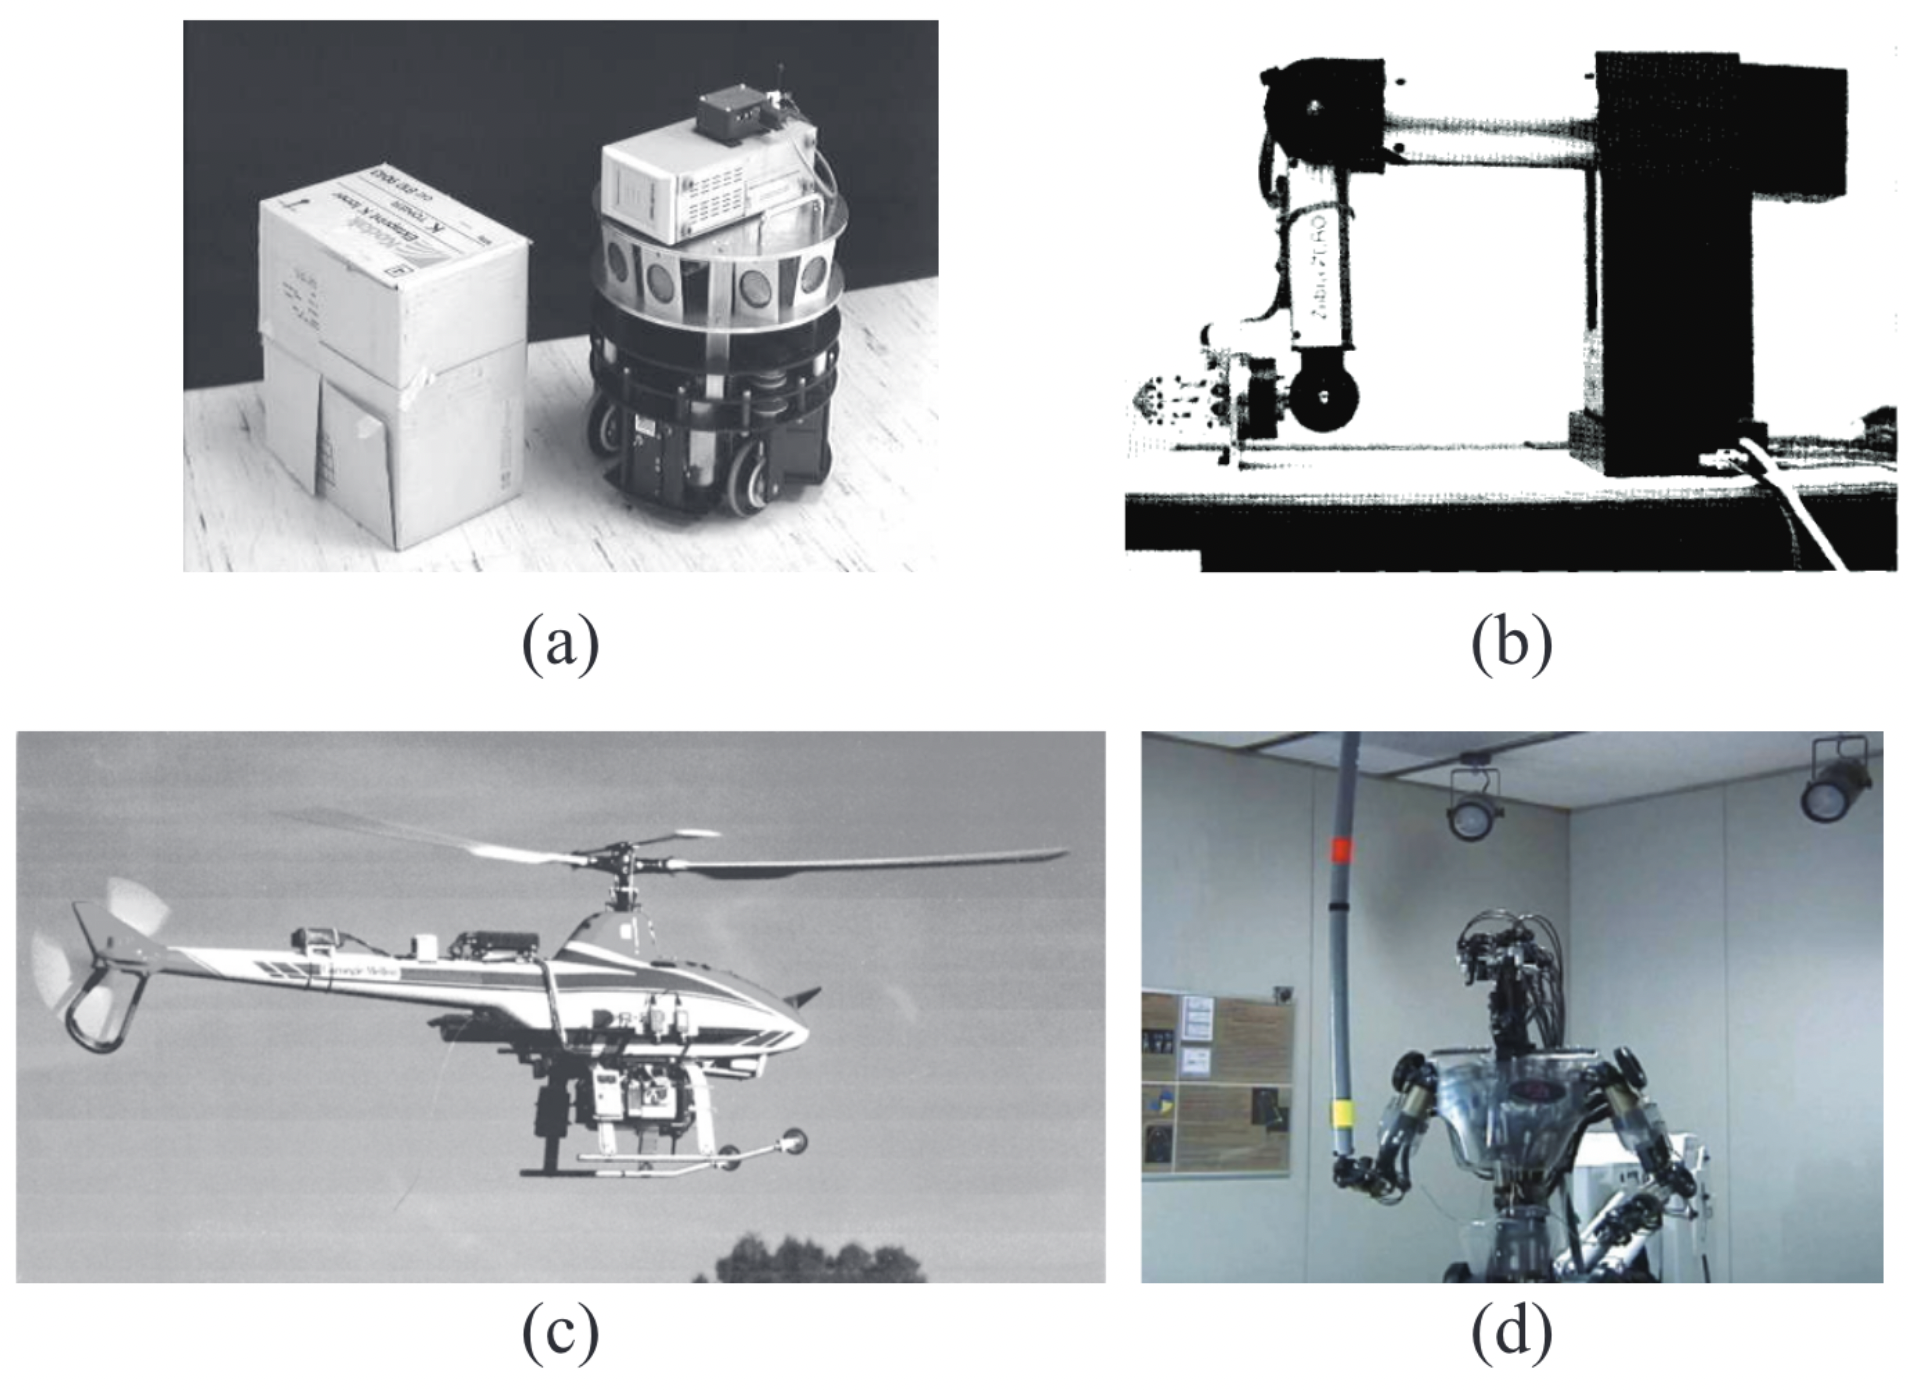
\includegraphics[width=14.70cm, height=10.0cm]{robots.png}
    \caption{Some of the robots that were used reinforcement learning algorithm. (a) OBELIX, (b) A Zebra Zero, (c) Carnegie Mellon's autonomous helicopter, (d) Sarcos}
\end{figure}

\noindent Additionally, Figure 3.23 illustrates the use of several RL-based learning techniques in robotics depending on usage as described in the literature. Let's now examine how RL is used in several types of robot literature:
\begin{itemize}
\item \textbf{Under-water Robots:} The autonomous underwater robot is particularly helpful in the research of deep sea, including minerals in the earth's crust and aquatic life. However, due to the dynamic environment, controlling the autonomous underwater robot is exceedingly challenging. For communication or the internet, cables are widely placed in the deep sea. In order to find faults or perform necessary maintenance, it is necessary to follow the wires. As a result, [92] have created a hybrid approach for cable tracking task employing a natural actor-critic (NAC) algorithm with $LSTD-Q(lambda)$. Another use [93] is that Nessie VII AUVs are subjected to an Actor-critic algorithm and DeepRL integrated framework for adaptive control. You can seen more applications in Table 3.1
\newpage    
\begin{table}[h!]
\centering
\begin{adjustbox}{width=1\textwidth}
\begin{tabular}{||c c c||} 
 \hline
 \textbf{Vehicle} &\textbf{Purpose} & \textbf{RL Method} \\ [0.5ex] 
 \hline\hline
 Ictineu AUV & Cable tracking mission & Hybrid RL: (NAC + $LSTD-Q(\lambda)$) \\ 
 \hline
 Ictineu AUV & Visual based cable tracking mission & Actor-critic \\
 \hline
 Nessie-VII AUV & Adaptive low-level control & DeepRL + actor-critic \\
 \hline
 Neptune-I AUV & Target based search & DeepRL + DQL based Dual stream Q-network \\
 \hline
 2vs2 water polo game & Coordinate between multiple AUVs & Multi-agent RL \\ [1ex]
 \hline
\end{tabular}
\end{adjustbox}
\caption{Application for Underwater Robots}
\end{table}

\item \textbf{Flying robots:} Numerous uses for flying robots have been discovered, including surveillance, emergency response, real-time communication, multi-coordination activities, etc. Future airborne robots must be able to navigate risky environments, such as those with turbulence in the air or a lost GPS connection, more intelligently. As a result, the vehicle must function effectively and independently using its onboard sensors. It might be very difficult to deliver time-sensitive commodities, like bodily organs, on time. For a rendezvous cargo delivery task by quad-copter, [94] have suggested a model-free based RL with continuous inputs. In which a quad-copter must carry a suspended load and transfer it swing-free to a land-based robot. UAVs can be used in a complicated catastrophe setting to conduct target-based searches. [95] suggested a DeeRL-based snake algorithm for finding objects that resembled injured individuals. You can seen more applications in Table 3.2

\begin{table}[h!]
\centering
\begin{adjustbox}{width=1\textwidth}
\begin{tabular}{||c c c||} 
 \hline
 \textbf{Vehicle} &\textbf{Purpose} & \textbf{RL Method} \\ [0.5ex]  
 \hline\hline
 Quadrotor & Rendezvous cargo delivery task & Model-free RL + Continuous inputs \\ 
 \hline
 Qball-X4 quadrotor & Planning of Construction task & Adaptive Scheme + RL + heuristic search \\
 \hline
 Quadrotor & Visual servoing & IBVS + fuzzy + Q-learning \\
 \hline
 Flocks of UAVs  & Learn control policy to follow leader & Q-learning + Peng's $Q(\lambda)$ \\
 \hline
 Multiple drones & Energy efficient cellular aided & DPG \\ [1ex]
 \hline
\end{tabular}
\end{adjustbox}
\caption{Application for Flying Robots}
\end{table}
\newpage
\item \textbf{Land Robots}: An autonomous land-based vehicle is a robot that runs without a human driver. The car is equipped with cutting-edge AI-based technologies. However, land robots have a variety of uses in the real world, including picking up goods, avoiding collisions in crowded spaces, operating on manufacturing sites, etc. It does, however, encounter several difficulties, such as environmental uncertainty and interruptions in feedback signals from vision-based sensors. A robust vision-based Q-learning controller for mobile robots on wheels has been developed [96]. Here, a feedback signal is sent from the vision sensor to the controller. Similar to this, a robotic goalkeeper for soccer is learned based on experience replay [97]. You can seen more applications in Table 3.3
\begin{table}[h!]
\centering
\begin{adjustbox}{width=1\textwidth}
\begin{tabular}{||c c c||} 
 \hline
 \textbf{Vehicle} &\textbf{Purpose} & \textbf{RL Method} \\ [0.5ex]  
 \hline\hline
 Simulated iCub robot & Automatic learning for various task & Q-Leaning \\ 
 \hline
 7-DoF arm of ABB Yumi & grasping, reaching and lifting objects  & DeepRL \\
 \hline
 18 DoF biped robot & Learning from walking patterns and adapt to terrain & Q-Leaning \\
 \hline
 Robotic soccer goalkeeper & Keeper learn to catch balls shot towards goal & EX-SARSA \\ [1ex]
 \hline
\end{tabular}
\end{adjustbox}
\caption{Application for Land Robots}
\end{table}
\end{itemize}

\begin{figure}[h]
    \centering
    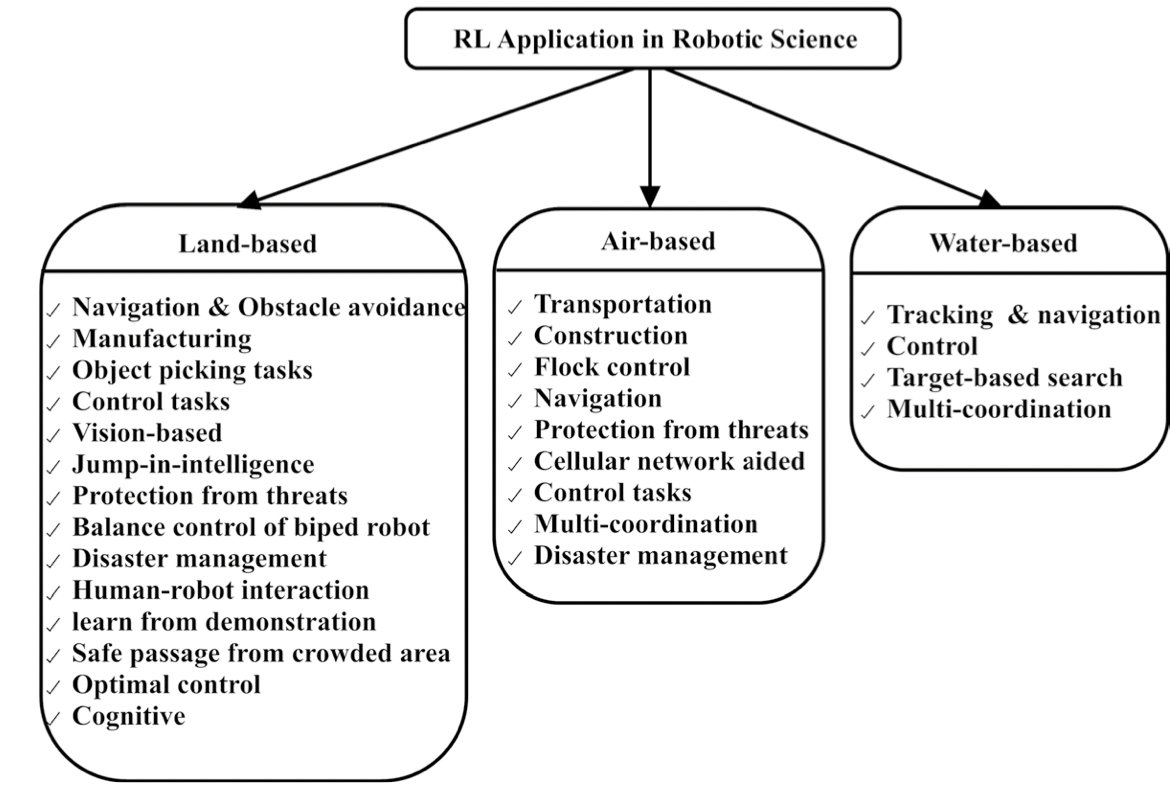
\includegraphics[width=14cm, height=9.0cm]{robots2.png}
    \caption{Reinforcement learning application of for Robots}
\end{figure}

\subsection{Fundamentals of Reinforcement Learning}
RL is when an artificial agent created in an unknown dynamic environment interacts with the environment to fulfill the determined task and collects reward values as a result of interaction. In the RL approach, the artificial agent aims to maximize or minimize the reward value it collects as a result of interaction with the environment. The artificial agent is in a state in the environment as a result of every interaction with the environment. The agent takes a series of actions and takes a decision when he is present. As a result of the decisions taken by the agent, he moves to a new state in the environment and as a result of this, the agent collects positive or negative rewards from the environment. It is expected that the collected rewards will reach the maximum level and that the artificial agent will learn to do the targeted work as a result of the sequential decisions made. This situation is cyclically seen in Figure 3.24.
\begin{figure}[h]
    \centering
    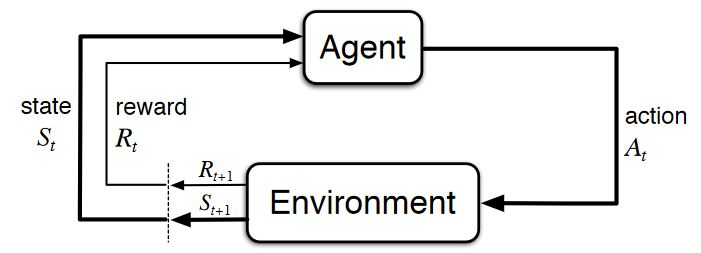
\includegraphics[width=14.0cm, height=5.0cm]{agent_rl.JPG}
    \caption{Interaction of agent and environment in a Markov decision process. [19]}
\end{figure}

\noindent In Figure 3.24, $R_t$ represents the reward received by the artificial agent from the environment. $A_t$ refers to the actions that the artificial agent has sent to the environment. $S_t$ refers to the states in which the artificial agent is in the environment. While the artificial agent is in the $S_t$ state at any time $t$, it performs the $A_t$ action and receives the reward of $R_{t+1}$ and accordingly switches to the $S_{t+1}$ state.

\subsection{Concepts Used in Reinforcement Learning}
\begin{itemize}
    \item \textbf{Agent}: A structure that senses/explores the environment and can act accordingly. In this project, our agent will be a robot.

    \item \textbf{Environment}: Where the agent resides and is connected to, the environment is such that the agent can learn and interact. The environment in which the agent is located is partially observable or fully observable. In reinforcement learning, the environment and observations of the agent can be random.
    
    \item \textbf{Action}: Actions can be thought of as decisions taken by the agent in the environment and are expressed by $a \in A$. The actions to be taken by the agent can be of continuous value or discrete value.
    
    \item \textbf{State}: The state holds information about how the agent is in the environment and is expressed as $s \in S$. It carries the minimum information necessary for the agent in the environment and is expressed in continuous time and discrete time according to the environment and the definition of the problem.
    
    \item \textbf{Reward}: Feedback from the environment as a result of the agent's actions. The reward can be positive or negative.
    
    \item \textbf{Policy}: The policy determines what action the agent in the state $s_t$ at time $t$ will choose from the action set $A_t$. The policy maps the current state $s_t$ to the action $a_t$. The policy strategy that the agent will follow can be modeled as deterministic or stochastic.
    
    \item \textbf{Trajectory}: It covers all the transitions between the current state and the next states, depending on the target that the agent realizes as a result of the reinforcement learning algorithm. With reinforcement learning, the set of states $\left\{s_1, s_2, ...., s_N \right\}$ forms our trajectory as the agent learns the specified target.
\end{itemize}

\subsection{Reinforcement Learning Models}
RL algorithms are classified into a wide variety. It is possible to divide RL into two classes, model-based and model-free. Model-based algorithms are built on a prior knowledge about the environment or a mathematical model that expresses the environment. Model-based RL is similar to model predictive control (MPC), which is the optimal control method. Model-free RL algorithms do not have any information about the environment. Algorithms are developed by modeling the environment with the Markov decision process, which is usually a random process. The artificial agent explores the environment and collects information about the environment and makes optimal decisions. This process constitutes the RL approach of trial, error and reward collection. RL is applied in many fields today, and one of the main reasons for its success is that it does not need a model about the environment. In this way, it solves many engineering problems by interacting with the environment. In this thesis, model-free RL algorithms will be emphasized, and model-based algorithms will be shortly mentioned.
\\ \\
Another classification of RL is on continuous or discrete state/action pairs. In this classification, the states of the environment in which the agent is located can be continuous time or discrete time. The actions taken by the agent to interact within the environment can be continuous and discrete. For robot and control problems, the state and action pair are mostly continuous. If the environment in which the agent is located consists of finite-dimensional discrete action and state pairs, RL algorithms produce solutions with algorithms based on table methods. If the environment or action pair with which the agent interacts takes continuous values, the algorithms proposed in the table method are not effective. In this thesis, algorithms created with continuous action/state pairs will be emphasized and discrete action/state pairs will be shortly mentioned. Since the control problem of the continuum robot is modeled with a continuous action and state pair, it has been decided to solve the problem with a DDPG algorithm [20].
\\ \\
Another classification of RL is value-based and policy-based algorithms. Value-based RL algorithms learn the values of performing a certain $a_t$ action in a $s_t$ state where the artificial agent is in the environment. In the value-based approach, the policy applied by the algorithms is that the agent chooses whichever has the highest return on the actions applied to the environment. Such an approach is called the greedy approach. The agent chooses whichever of the actions it performs in its states provides the greatest return. Thus, the policy of the agent is called the greedy approach. In policy-based RL algorithms, it aims to discover the appropriate policy instead of learning the values of the $s_t$ states that the agent is in. In this approach, unlike the greedy approach followed by the agent, it is aimed to ensure that appropriate decisions are made in each state. Thus, the agent develops a behavior by learning the policy in the environment it is in. Algorithms differ according to the problem applied, with the value-based approach and the policy-based approach. There are RL algorithms in which value-based and policy-based approaches are used together. In such a case, the agent learns the value of being in the $s_t$ state and the appropriate policies. The DDPG algorithm proposed in this thesis comes from both value and policy based algorithm families.
\\ \\
There are other types of RL such as on-policy and off-policy methods in addition to this classification, but more will not be discussed.

\subsubsection{Model-based Reinforcement Learning}

Since we have a complete mathematical model of the environment in the model-based approach, one of the RL approaches, we can reach the conclusion with a comprehensive search algorithm, that is, by searching all possible outcomes. Because of the computational complexity, the search process can be applied in simple applications such as tic-tac-toe game. The search complexity increases depending on the conditions and actions of the environment. Finding results by search is impractical for many problems, assuming that the size of our probable state space about a state $s = 100$ is $2^{100}$ and the possible actions for each state are known, assuming the environment model knows. Where we have a mathematical model of the environment, another approach used for the solution is dynamic programming. In dynamic programming, it allows us to iteratively solve the optimal policy instead of searching extensively depending on possible states and actions. Dynamic programming allows us to develop a methodology for the optimal solution and iteratively calculates the solution. If we have a precise knowledge of the environment, dynamic programming and comprehensive search approaches guarantee optimal policy. 
\\ \\
Most RL approaches assume that there is no detailed prior knowledge about the environment and that some algorithms cannot access all states of the environment (POMDP). When the systems established in the physical world are considered, there are mostly undetectable dynamics, noise, etc. that change over time. For these reasons, many physical systems exhibit stochastic behavior. Although the dynamic programming approach is deterministic or stochastic, it needs a mathematical model. Thanks to the model-free approach of RL, an approximate solution of dynamic programming is created. Dynamic programming is implemented in the optimal control problem. It creates the optimal policy, that is, the control signal, by minimizing a certain objective function.

\subsubsection{Model-Free Reinforcement Learning}
Maximizing or minimizing the reward collected by the artificial agent, thanks to the reward function created by interacting with the environment is our aim in model-free approach. In model-free RL, two basic approaches, which are called Monte Carlo (MC) and Temporal Difference (TD), are used. 
\\ \\
In MC approach, the algorithm does not update itself until it reaches the final state at the end of a episode or in the environment. When the end of the episode is reached, an update of the algorithm will be created.
\\ \\
In the temporal difference method, the algorithm is updated at a certain time interval. Temporal difference algorithms are usually expressed as $TD$ and mathematically expressed as $TD(0)$ ,$TD(1)$. Depending on the expression format, the most common notation is $TD(\lambda)$, $\lambda \ in [0,1]$. The $TD(0)$ approach states that we are only looking one step ahead as a temporal difference. The $TD(1)$ approach is equivalent to the Monte Carlo approach, meaning we create an update at the end of the section. Thus, in $TD(\lambda)$ the term $\lambda$ indicates what kind of horizon the algorithm will examine in the future. Differences between $TD(0)$ and $TD(1)$ $= MC$ method, $MC$ method has high variance while $TD$ method has low variance. This is because the $MC$ method updates over the entire action state pair during a segment, while the $TD$ method has a one-step update rule. The $MC$ method has a low bias value because it considers a partition to update the parameters, while the $TD$ method has a high bias value because it proceeds through instant updates. The algorithms examined in this thesis were created using the $TD$ method. The $TD$ method basically has two basic algorithms as Sarsa and Q learning algorithms. The differences between MC, TD and Dynamic Programming are shown in Figure 3.25 [19].
\begin{figure}[h]
    \centering
    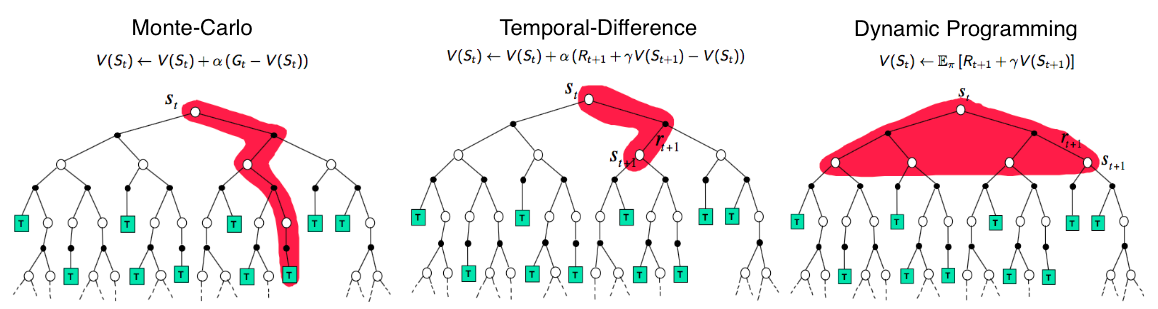
\includegraphics[width=16.0 cm, height=4.5cm]{TD_MC_DP.png}
    \caption{Reinforcement Learning Methods [21]}
\end{figure}

\subsection{Exploration/Exploitation trade-off}
It is assumed that the agent has no knowledge of the environment in the model-free approach. The agent have to first explore the environment to interact and make decisions. The agent needs to travel around the environment in order to decide on the reward values according to the states and states in the environment and to create the optimum policy. Suppose we start with an estimate of zero value for each state and action pair. As soon as we take an action that yields a positive reward, an algorithm that follows the greedy policy will continue to execute that action undisturbed. Our RL algorithm will get stuck at the local minimum point before it is determined whether the action is optimal or not. In this case, the artificial agent has to conform to the concept of exploration and exploitation without making a decision. \\ \\
It is possible that there will be sub-optimal policies that are sub-optimal than the optimal policy the agent finds. The agent should search the environment by navigating with the random value at the beginning and explore the environment thoroughly. After accessing almost all the dynamics about the environment, providing access to values and starting to make optimal decisions, our algorithm should abandon the exploration approach and move towards the exploitation approach, that is, use the knowledge it has acquired before. As it will be remembered, model-free approaches do not guarantee the optimal policy like DP, which is a model-based algorithm. In the model-free approach, the agent is expected to interact with the environment and make the most optimal decisions to create the optimal policy. In the exploration phase of the algorithm, it should exhibit random behavior, roam stochastically in the environment, and collect all the bad and good results. In the exploitation phase, our algorithm must act on decisions with the highest values. In RL, our algorithms are expected to balance well between exploration and exploitation. In a static environment, our algorithm is expected to follow the appropriate policy based on maximum exploration at the start, and after the learning phase, based on its experience. The $\epsilon - greedy$ approach is used to mathematically establish the balance between exploration and exploitation. In this approach, the agent initially performs a probabilistic action with the value of $\epsilon \in [0,1]$, applying a maximum level of random action, thus discovering its environment. As time progresses, the value of $\epsilon$ shows an exponential decrease and is less exploratory and enters the exploitation stage. Thus, as learning takes place, it is ensured that the algorithm uses its experiences [22].

\subsection{Reinforcement Learning and Control Theory}
The main problem of control theory is to follow the target reference signal by generating the appropriate control signal for a physical system. The block diagram of a classical closed loop control system is shown in Figure 3.26.
\begin{figure}[h]
    \centering
    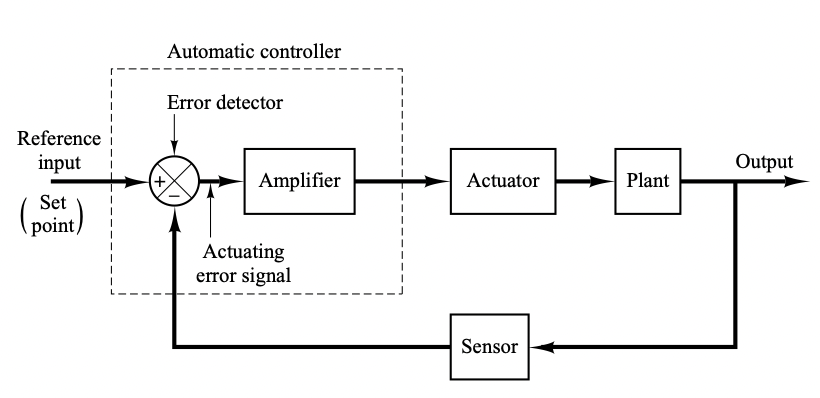
\includegraphics[width=12.4 cm, height=6.0cm]{control.png}
    \caption{Block diagram of a control system [23]}
\end{figure}

\noindent It is possible to control physical systems with the general control structure in Figure 3.26. In control theory, if there is a mathematical model of the physical system, it is possible to create a model-based control system.
\\ \\
In cases where the model of the physical system is unknown, system identification techniques are used in the classical control theory approach. Distorting inputs, noise and unmodelable dynamics affecting the physical system affect the performance of the generated controller. Optimal control theory can be considered as the optimal control that will meet a certain performance criterion by examining the previous section. In the optimal control theory, having a model of the physical system and making optimal decisions are similar to the model-based RL concept. The advantage of RL over optimal control theory is that we can write the reward function freely. In optimal control theory, the objective function consists of certain functions and the solution is formed according to these functions. The control sign $u(t)$ created in control theory constitutes the actions $a(t)$ in RL. The controller designed in control theory corresponds to the policy in RL. Controllers created in control theory vary according to the physical system and control performance. Model predictive control (MPC), linear quadratic regulator (LQR), etc. methods have been proposed in the literature to create an optimal controller. 
\\ \\
In cases where the controller should be robust or adaptive, control methods such as Hinf, MRAC etc. have been suggested. PID controllers are used in many industrial systems. The advantage of the PID controller is that it is parameterized empirically and is independent of the mathematical model of the physical system. The environment created in RL opposes the dynamic equations of the physical system and is usually expressed in the form of nonlinear time-varying stochastic differential equations. In the physical world, many systems are automatically controlled by model-based control algorithms. Today, control theory forms the basis of industry and industry in many fields such as autonomous vehicles, rocket systems, airplanes, robots, etc. Control theory is very powerful because it generates analytical solutions when mathematical models are specific. 
\\ \\
In this thesis, the mathematical model of the continuum robot was created, and it was made to reach the target point. In order to establish control systems, the mathematical models of the physical system must be written very well. The created controller is expected to exhibit optimal or adaptive control performance. In control theory, the inability to establish models of physical systems or the uncertainties in the system pose a problem. In robotics, manipulators and their models contain many problems. In order to solve problems such as grasping, imitating human movements in robotics, strong mathematical modeling and control knowledge is needed. The algorithms created do not always offer the best performance. With the development of ML and RL, the difficulties and problems encountered in control theory are solved. In this thesis, the continuum robot control problem created in Chapter 6 is solved by RL algorithm. Thus, optimal solutions have been created independent of the physical system and disruptive inputs. Thanks to the reward functions written flexibly for RL, many optimal controls suitable for physical systems are created [22].

\subsection{Stochastic Processes and Markov Process}
In this thesis, model-free RL algorithms using the temporal difference method will be examined. The mathematical models of physical systems are written with a nonlinear differential equation can be seen in equation 3.1a and 3.1b.
\begin{subequations}
\begin{align}
        \dot{x}(t) = f(t,x,u,w), \\ 
        y(t) = g(t,x,u,v)
\end{align}
\end{subequations}
In Equation 3.1, time $t$, state vector $x$, control signal $u$, process noise $w$ measurement noise $f(.)$ nonlinear differential equations generated from the system model, $g(. ) $ creates the output equation. If the solution of the mathematical model of the physical system is known, states can be obtained through the state transition matrix. However, many physical systems cannot be solved due to uncertainty, noise, and unmodelable dynamics.
\\ \\
There are often no analytical solutions for nonlinear models of physical systems. In order to construct the mathematical model of the system with random processes, the states of the system $x'$s are expressed as random variables. Thus, transitions between states are modeled in a stochastic fashion. With the RL approach, it models the transitions between physical systems and their states with the Markov decision process, which is a random process. In engineering and scientific applications, random events appear in the form of a series. A random sequence of events can be expressed in one- or multidimensional functions of time or location. In such cases, modeling is done with the concept of random process. The random process is mathematically expressed as $X(t), X(n)$. The collection of functions created by assigning a function to each event in the probability space according to a certain rule is called a random process or stochastic process. In the collection of functions expressing the random process, simple (PDF) or joint probability density functions (JPDF), this process is called stationary if it does not change over time. In stationary processes, all moments of the process are independent of time. In some cases, functions expressing the random process exhibit the same statistical properties. This means that the random process has the characteristic of ergodicity. In such special cases, the statistical properties of the whole process can be modeled by knowing a single sample function that represents the random process in the implementations of the process. Random processes are examined in four classes as discrete-valued discrete-time random process, discrete-valued continuous-time random process, continuous-valued discrete-time random process, and finally, continuous-valued continuous-time random process. Within the scope of this thesis, for simplycity is a discrete-valued discrete-time Markov process and the extended cases of the Markov process will be examined. Random processes satisfying Equation 3.2 are called Markov processes.
\begin{subequations}
\begin{align}
        P\left[X\left(t_{k+1}\right)=x_{k+1} \mid X\left(t_{k}\right)=x_{k}, \ldots, X\left(t_{1}\right)=x_{1}\right] \\ =P\left[X\left(t_{k+1}\right)=x_{k+1} \mid X\left(t_{k}\right)=x_{k}\right]
\end{align}
\end{subequations}
As can be seen from Equation 3.2, the $X\left(t_{k+1}\right)$ value of the random process $X(t)$ depends on a historical value of $X(t)$. This property is called the Markov property. Random processes that provide this feature are called Markov processes. In Equation 3.2, $t_{1}<t_{2}<t_{3}<\ldots<t_{k}<t_{k+1}$ represents the time index. If the joint probability density function (JPDF) of the random process is known, the Markov process is expressed by the state transition matrix. This situation is seen in Equation 3.3.
\begin{subequations}
\begin{align}
        P\left[X_{n+1}=j \mid X_{n}=i\right]=p_{i j}
\end{align}
\end{subequations}
In Equation 3.3, $X_{n}$ are called homogeneous transition probabilities. By giving the common probability density function $X_{n}, \ldots, X_{0}$, Equation 3.3 can be expressed as in equation 3.4.
\begin{subequations}
\begin{align}
        P\left[X_{n}=i_{n}, \ldots, X_{0}=i_{0}\right]=p_{i_{n-1}, i_{n} \ldots} p_{i_{0} i_{1}} p_{i_{0}}(0)
\end{align}
\end{subequations}
Thus, the transition probabilities matrix $P$ is obtained as in Equation 3.5 if the initial values $p_{i}(0)$ are given.
\begin{subequations}
\begin{align}
        P=\left[\begin{array}{cccc}
        p_{00} & p_{01} & p_{2} & \cdots \\
        \vdots & \vdots & \cdots & \cdots \\
        \vdots & \vdots & \cdots & \cdots \\
        p_{i 0} & p_{i 1} & \cdots & \cdots
        \end{array}\right]
\end{align}
\end{subequations}
The sum over the columns of the state transition matrix expressed in Equation 3.5 should make one. The column sum expression is seen in Equation 3.6.
\begin{subequations}
\begin{align}
        \sum_{j} P\left[X_{n+1}=j \mid X_{n}=i\right]=\sum_{j} p i j=1
\end{align}
\end{subequations}
\newpage
\noindent Figure 3.27 shows an example for a two-state Markov process.
\begin{figure}[h]
    \centering
    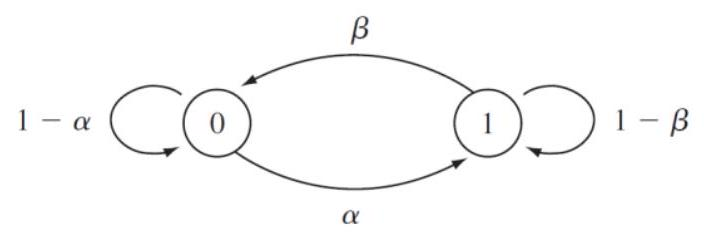
\includegraphics[width=7.9 cm, height=3.0cm]{markov.jpg}
    \caption{Two State Markov Chain State Transition Diagram }
\end{figure}

\noindent The state transition matrix of the two-state Markov chain expressed in Figure 3.27 is expressed by Equation 3.7.
\begin{subequations}
\begin{align}
        P=\left[\begin{array}{cc}
        1-\alpha & \alpha \\
        \beta & 1-\beta
        \end{array}\right]
\end{align}
\end{subequations}
In order to calculate the bistable Markov chain expressed in Figure 3.27 over time, the powers of equation 3.7 must be taken. This situation is as in Equation 3.8 for n step calculation.
\begin{subequations}
\begin{align}
        P^{n}=\underbrace{\left[\begin{array}{cc}
        1-\alpha & \alpha \\
        \beta & 1-\beta
        \end{array}\right]\left[\begin{array}{cc}
        1-\alpha & \alpha \\
        \beta & 1-\beta
        \end{array}\right] \cdots\left[\begin{array}{cc}
        1-\alpha & \alpha \\
        \beta & 1-\beta
        \end{array}\right]}_{n}
\end{align}
\end{subequations}
With Equation 3.8, the state transition probabilities with steps $\mathrm{n}$ can be calculated by knowing the state transition matrix $P$. If a random process $X_{k}$ is independent and expressed with the same probability distribution, this process is expressed as IID, and the equation is mathematically expressed as Equation 3.9.
\begin{subequations}
\begin{align}
        &F_{X_{1}, X_{2}, \ldots, X_{k}}\left(x_{1}, x_{2}, \ldots, x_{k}\right)=P\left[X_{1} \leq x_{1}, X_{2} \leq x_{2}, \ldots, X_{k} \leq x_{k}\right], \\
        &F_{X_{1}, X_{2}, \ldots, X_{k}}\left(x_{1}, x_{2}, \ldots, x_{k}\right)=F_{X}\left(x_{1}\right) F_{X}\left(x_{2}\right) \ldots F_{X}\left(x_{k}\right)
\end{align}
\end{subequations}
Equation 3.9 expresses the statistical independence of random variables $X_{k}$. For the RL algorithms created in this section, the data obtained by the agent from the environment should not be IID. The problem of getting stuck in the local point of the algorithms created with the data obtained in this way is eliminated [24].

\subsection{Markov Reward Process}
In the RL approach, it is assumed that the mathematical model of the environment in which the artificial agent is located is not known. The transition between the environment and states of the artificial agent is modeled by Markov reward processes, which are an extended version of the Markov process. Within the scope of this thesis, it is assumed that the environment states are fully accessible. In the absence of full access to the environment states, Markov decision processes are called partially observed Markov decision processes. The Markov property and the state transition probability matrix are as in Equation 3.10.
\begin{subequations}
\begin{align}
    \begin{gathered}
    P\left[S_{t+1} \mid S_{t}\right]=P\left[S_{t+1} \mid S_{1}, S_{2}, \ldots, S_{t}\right], \\
    P=\left[\begin{array}{ccc}
    P_{11} & \cdots & P_{1 n} \\
    \vdots & \ddots & \vdots \\
    P_{n 1} & \cdots & P_{n n}
    \end{array}\right]
    \end{gathered}
\end{align}
\end{subequations}
It can be seen from Equation 3.10 that the random process providing the Markov property is memoryless. The Markov process or Markov chain is defined by $(S, P)$. $S$ represents the finite state space. $P$ is the state transition probabilities matrix. It is expressed mathematically by $P_{s s^{\prime}}=$ $P\left[S_{t+1}=s^{\prime} \mid S_{t}=s\right]$ and $s ^{\prime}$ denotes the next state. $P_{s s^{\prime}}$ represents the transition probability $s \rightarrow s^{\prime}$. The Markov reward process is an extended version of the Markov process with the value expression. Markov reward process $(S, P, R, \gamma), S, P$ denotes the reward function $R$, as specified in the Markov process, $R_{s}=E\left[R_{t+1} \mid S_ {t}=s\right]$ takes a value in the range of $\gamma \in [0,1]$ as a reduction factor of $\gamma$. The $G_{t}$ function defined in the Markov reward process expresses the total reduced reward over the time step and is defined mathematically as in Equation 3.11.
\begin{subequations}
\begin{align}
    G_{t}=R_{t+1}+\gamma R_{t+2}+\ldots=\sum_{k=0}^{\infty} \gamma^{k} R_{t+k+1}
\end{align}
\end{subequations}
The $\gamma$ parameter expressed in Equation 3.11 expresses how much the value of the $G_{t}$ reward function depends on future rewards. For $\gamma=0$, the algorithm depends on the $R_{t+1}$ reward it has received at the time $t$ is found. For $\gamma=1$, the $G_{t}$ reward function is dependent on all future rewards. The $\gamma$ parameter establishes the balance between the future and the present. The MPC algorithms used in optimal control theory are called horizon control. The control horizon expression created here indicates how many future examples the optimization process should cover1. With the model-independent approach used in RL, since the artificial agent does not know the environment and the reward it will receive depending on the environment, it is necessary to establish a connection between the future and the present. The $\gamma$ parameter provides the balance between future and present rewards. Value method is used to solve the Markov reward process. The value function approximation is seen in Equation 3.12.
\begin{subequations}
\begin{align}
    V(s)=E\left[G_{t} \mid S_{t}=s\right]
\end{align}
\end{subequations}
The value function $V(s)$ in Equation 3.12 constitutes the expected value of the $G_{t}$ function expressed by equation 3.11. The value function divides 3.12 into two parts. This situation is seen in Equation 3.13.
\begin{subequations}
\begin{align}
    &V(s)=E\left[G_{t} \mid S_{t}=s\right], \\
    &\quad=E\left[R_{t+1}+\gamma R_{t+2}+\gamma^{2} R_{t+3}+\ldots \mid S_{t}=s\right], \\
    &\quad=E\left[R_{t+1}+\gamma\left(R_{t+2}+\gamma R_{t+3}+\ldots\right) \mid S_{t}=s\right], \\
    &\quad=E\left[R_{t+1}+\gamma G_{t+1} \mid S_{t}=s\right], \\
    &\quad=E\left[R_{t+1}+\gamma V\left(S_{t+1}\right) \mid S_{t}=s\right]
\end{align}
\end{subequations}
Equation $3.13$ is the value function expressed in Equation 3.12, expressed as Bellman's equation. The Equation 3.13, expressed as a system of linear equations, can be seen in equation 3.14.
\begin{subequations}
\begin{align}
    V(s)=R_{t}+\gamma \sum_{s^{\prime} \in S} P_{s s^{\prime}} V(s)
\end{align}
\end{subequations}
Knowing the Equation 3.14 with the reward function $R_{t}$ and the state transition matrix $P_{s s^{\prime}}$, the value of being in the $s$ state for the Markov reward process can be calculated. The Bellman equation, expressed as in Equation 3.14, can be written as a matrix vector as seen in Equation 3.15.
\begin{subequations}
\begin{align}
    \left[\begin{array}{c}
V(1) \\
\vdots \\
V(n)
\end{array}\right]=\left[\begin{array}{c}
R_{1} \\
\vdots \\
R_{n}
\end{array}\right]+\gamma\left[\begin{array}{ccc}
P_{11} & \cdots & P_{1 n} \\
\vdots & \ddots & \vdots \\
P_{n 1} & \cdots & P_{n n}
\end{array}\right]\left[\begin{array}{c}
V(1) \\
\vdots \\
V(n)
\end{array}\right]
\end{align}
\end{subequations}
The solution of the Markov reward process using equation 3.15 is as seen in equation 3.16.
\begin{subequations}
\begin{align}
    V &=R+\gamma P V, \\
    (1-\gamma P) V &=R, \\
    V &=(1-\gamma P)^{-1} R
\end{align}
\end{subequations}
With equation $3.16$, the value function $V$ can be calculated. Thus, in the environment modeled by the Markov reward process, the rewards for the presence of the artificial agent in each state are calculated. The value function $V(s)$ depends on the state set $s \in S$. Since the Markov reward process is discrete-state discrete-valued, it has a finite set of countable states. Equation 3.16 The solution can be calculated for a limited number of state values. The computational complexity value of Equation 3.16 is $n$ states $O\left(n^{3}\right)$. For very large size MRP, iterative solution methods, dynamic programming, monte carlo method and temporal difference method are used for solution [22].

\subsection{Markov Decision Process}
The Markov decision process is the extension of the Markov reward process with the action set $a \in A$, and mathematically, the finite and discrete state set $S$ provides the Markov property, the action set $A$, $P_{s s^{\prime}}^ {a}=P\left[S_{t+1}=s^{\prime} \mid S_{t}=s, A_{t}=a\right]$
conditional pass probability is defined by the reward function $R_{s}^ {a}=E\left[R_{t+1} \mid S_{t}=s, A_{t}=a\right]$ and the discount factor $\gamma \in[0,1]$ . Two important approaches identified in the Markov decision process are policy and value functions. The policy is denoted by $\pi$. The policy is mathematically seen in equation 3.17.
\begin{subequations}
\begin{align}
    \pi(a \mid s)=P\left[A_{t}=a \mid S_{t}=s\right]
\end{align}
\end{subequations}
The policy expressed by the equation $3.17$ expresses the agent's taking action $a$ in the case of $s$, that is, the behavior of the agent. In MDP, policy is based on the $s_{t}$ state the agent is in, not on future or past states. Policy is time independent. This situation is seen in equation 3.18.
\begin{subequations}
\begin{align}
    A_{t} \sim \pi\left(. \mid S_{t}\right) \forall t>0
\end{align}
\end{subequations}
Given the Markov decision process $M=(S, A, P, R, \gamma)$ and a policy $\pi$, the states $S_{1}, S_{2}, \ldots$ Markov property $\left(S , provides P^{\pi}\right)$. State and reward values $S_{1}, R_{1}, S_{2}, R_{2}, \ldots$ Markov decision process $\left(S, P^{\pi}, R^{\pi } denotes \gamma\right)$. In equation 3.19, $P^{\pi}, R^{\pi}$ are mathematically defined.
\begin{subequations}
\begin{align}
    P_{s s^{\prime}}^{\pi} &=\sum_{a \in A} \pi(a \mid s) P_{s s^{\prime}}^{a}, \\
    R_{s}^{\pi} &=\sum_{a \in A} \pi(a \mid s) R_{s}^{a}
\end{align}
\end{subequations}
Another expression defined in the Markov decision process is the value function. The state value function is mathematically expressed in equation 3.20.
\begin{subequations}
\begin{align}
    V_{\pi}(s)=E_{\pi}\left[G_{t} \mid S_{t}=s\right]
\end{align}
\end{subequations}
Equation 3.20 shows the state-value function. The artificial agent expresses the rewards it will receive by starting from any $s$ state and following a certain policy $\pi$ in the environment modeled by the Markov decision process. Another defined function in the Markov decision process is the action-value function and is expressed mathematically as in equation 3.21.
\begin{subequations}
\begin{align}
    q_{\pi}(s, a)=E_{\pi}\left[G_{t} \mid S_{t}=s, A_{t}=a\right]
\end{align}
\end{subequations}
In Equation 3.21, the artificial agent expresses the reward values it receives as a result of starting from any $s$ state in the environment modeled by the Markov decision process, following a certain policy $\pi$ and applying a certain action $a$. As a result of the agent collecting actions and rewards in the environment in the Markov decision process, the Markov decision process has two different solution approaches. The expression of the state-value and action-value functions created in the Markov decision process, which was converted into Bellman's equation iteratively, is mathematically expressed in equations $3.22$ and $3.23$, respectively.
\begin{subequations}
\begin{align}
    V_{\pi}(s)=E_{\pi}\left[R_{t+1}+\gamma V_{\pi}\left(S_{t+1}\right) \mid S_{t}=s\right]
\end{align}
\end{subequations}
Equation 3.22 represents the creation of the state-value function with the Bellman equation. With this approach, the state-value function $V_{\pi}(s)$ can be calculated in a given case $S_{t}=s$ following a certain policy $\pi$.
\begin{subequations}
\begin{align}
   q_{\pi}(s, a)=E_{\pi}\left[R_{t+1}+\gamma q_{\pi}\left(S_{t+1}, A_{t+1}\right) \mid S_{t}=s, A_{t}=a\right]
\end{align}
\end{subequations}
Equation 3.23 expresses the action-value function. Thanks to this equation, the artificial agent expresses the values it receives as a result of applying $S_{t}=s \quad A_{t}=a$ by following a certain policy $\pi$ in the environment modeled by the Markov decision process. The linear equation system solution of equation 3.22 is as expressed in equation 3.24.
\begin{subequations}
\begin{align}
   &V_{\pi}=R^{\pi}+\gamma P^{\pi} V_{\pi}, \\
   &V_{\pi}=\left(1-\gamma P^{\pi}\right)^{-1} R^{\pi}
\end{align}
\end{subequations}
In the Markov reward process, there is the solution of the value function expressed in equation 3.16, just as the solution of the value function expressed in equation 3.16, in the Markov decision process, there is a solution of the value function expressed in equation 3.24. The application of the solution of equation 3.24 is possible by knowing the transition probabilities matrix $P^{\pi}$ for a finite number of $S$ states. In case the transition probability matrix is not known, approximate dynamic programming method, temporal difference method, and monte carlo method, which are approximate solutions of MDP, are used as approximate solutions. 3.22 optimal solution of the state value function expressed in the Markov decision process is expressed in equation 3.25.
\begin{subequations}
\begin{align}
   V_{*}(s)=\max _{\pi} V_{\pi}(s)
\end{align}
\end{subequations}
With Equation 3.25, the optimal value function $V_{*}(s)$ of the MDP is calculated by choosing the maximum of all policy values. Similarly, the optimal action value function is calculated by equation 3.26.
\begin{subequations}
\begin{align}
   q_{*}(s, a)=\max _{\pi} q_{\pi}(s, a)
\end{align}
\end{subequations}
Equation 3.25 expresses the best result in the optimal state-value function MDP. The optimal state-value function equation 3.25 forms the solution of the Markov decision process. Similar to solving MDP with optimal state-value function, MDP can be solved by determining the optimal action-value function given by equation 3.26. Thus, there are two different solution approaches of Markov decision processes: state-value and action-value. The optimal state value function is defined as in equation 3.27 over successive policies.
\begin{subequations}
\begin{align}
   \pi \geq \pi^{\prime} \quad V_{\pi}(s) \geq V_{\pi^{\prime}}(s) \quad \forall s
\end{align}
\end{subequations}
In Equation 3.27, if a policy value $\pi$ is greater than $\pi^{\prime}$ than the policy value in the next state, then the state-value functions following these policy values are also greater than and equal over all states. In the Markov decision process, there is an optimal policy $\pi_{*}$ which provides $\pi_{*} \geq \pi \forall \pi$. The optimal policy value provides the optimal state-value function. This situation is expressed mathematically by equation 3.28.
\begin{subequations}
\begin{align}
   V_{\pi_{*}}(s)=V_{*}(s)
\end{align}
\end{subequations}
Similar to Equation 3.28, all optimal policy value provides the optimal action-value function. This situation is expressed mathematically in equation 3.29.
\begin{subequations}
\begin{align}
   q_{\pi_{*}}(s, a)=q_{*}(s, a)
\end{align}
\end{subequations}
The optimal policy value can be found by equation 3.30 as the value maximizing $q_{*}(s, a)$.
\begin{subequations}
\begin{align}
   \pi_{*}(a \mid s)=\left\{\begin{array}{lc}
1 & a=\underset{a \in A}{\arg \max } q_{*}(s, a) \\
0 & \text { Otherwise }
\end{array}\right.
\end{align}
\end{subequations}
It will be recalled that a policy specifies how the dummy agent chooses action $a \in A$ in case $s$. Optimal policy choice is determined in the expression with Equation 3.30. Depending on the policy value, equation 3.28 optimal state-value function and equation 3.29 optimal action-value functions can be calculated. An optimal policy value can be determined for the Markov decision process. Bellman's recursive computational relation1 between equations 3.29 and 3.28 is expressed by equation 3.31.
\begin{subequations}
\begin{align}
   V_{*}(s)=\max _{a} q_{*}(s, a)
\end{align}
\end{subequations}
Equation 3.31 equates the optimal state-value function with the optimal action-value functions, following the optimal policy expressed in equation 3.30. The optimal state-value function is expressed by the Bellman equation as in 3.32.
\begin{subequations}
\begin{align}
   V_{*}(s)=\max _{a} R_{s}^{a}+\gamma \sum_{s^{\prime} \in S} P_{s s^{\prime}}^{a} V_{*}\left(s^{\prime}\right)
\end{align}
\end{subequations}
Similar to equations 3.31 and 3.323, the optimal action-value function is expressed in terms of the optimal state-value function as in equation 3.33.
\begin{subequations}
\begin{align}
   q_{*}(s, a)=R_{s}^{a}+\gamma \sum_{s^{\prime} \in S} P_{s s^{\prime}}^{a} V_{*}\left(s^{\prime}\right)
\end{align}
\end{subequations}
Combining equation 3.33 with equation 3.31, the optimal action-value function is written as expressed in equation 3.34.
\begin{subequations}
\begin{align}
   q_{*}(s, a)=R_{s}^{a}+\gamma \sum_{s^{\prime} \in S} P_{s s^{\prime}}^{a} \max _{a^{\prime}} q_{*}\left(s^{\prime}, a^{\prime}\right)
\end{align}
\end{subequations}
Equations 3.32 and 3.34 are proposed for iterative solutions of the state-value and action-value functions of the Markov decision process. With the solutions of these equations, the optimum values of the Markov decision process are calculated. The solution of Bellman's optimal equation is in non-linear form and has no analytical solutions in closed form. In the equation, the artificial agent $P_{s s^{\prime}}^{a}$ does not know. In $\mathrm{In this}$ case, equation 3.34 and equation 3.32 are solved by iterative methods. In the next section, value-based and policy-based approaches, which are iterative solutions of Markov decision processes, will be examined [25].

\subsection{Markov Decision Process Solution}
The Markov decision process can be expressed mathematically with the parameters $M=(S, A, P, R, \gamma)$. Here, $S$ states, $A$ actions, $P$ state transition probability matrix, $R$ reward function, and finally $\gamma$ reduction factor. In the Markov decision process, $P, R$ may be unknown, or the states may be in continuous time and cannot be calculated. Equations 3.34 and 3.32 were defined for the MDP solution, a deterministic policy $\pi:S \rightarrow A$ maps states to actions. In $\mathrm{In this}$ situation, it is mathematically defined and deterministic how the artificial agent will make and implement a decision in a state. A stochastic policy is defined by $\pi: S \boldsymbol{x} A \rightarrow$ $[0,1]$ and maps the decisions made by the decision maker in a given state to a certain probability value. For the solution of MDP, the artificial agent has to calculate the optimum value of the state-value approach and the optimum value of the action-value approach by following a certain policy. The value function that the agent will create by following a policy $\pi$ in a certain state by extending the value function with the Bellman equation is seen in equation 3.35.
\begin{subequations}
\begin{align}
   \widehat{V}_{\pi}(s)=R(s)+\lambda \sum_{s \in S} P\left(s^{\prime} \mid s, \pi(s)\right) \hat{V}_{\pi}\left(s^{\prime}\right)
\end{align}
\end{subequations}
The optimal state value function is determined as the optimal policy $\pi_{*}$ and calculated as in equation 3.36.
\begin{subequations}
\begin{align}
   \hat{V}_{*}(s)=R(s)+\gamma \max _{a \in A} \sum_{s^{\prime} \in S} P\left(s^{\prime} \mid s, a\right) \hat{V}_{*}\left(s^{\prime}\right)
\end{align}
\end{subequations}
Value-based solution of the Markov decision process with appropriate policy is expressed by equation 3.35. The value-based solution of the Markov decision process is expressed in equation 3.36. Equation 3.36 creates a solution over the values of the states in the Markov decision process. It should be noted that when calculating the sum of future discounted rewards, it processes the value at which the actions are maximum. The policy greedy approach used in the value-based approach is $(\varepsilon-$greedy). In Equation 3.35, in the policy-based approach, a solution is created by following a specific policy in each case. 
\\ \\
In the Markov decision process, approximate solutions are generated when $R, P$ are not known. Equations 3.35 and 3.36 constitute the value-based solutions of the Markov decision process. Another solution method in the model-based approach of RL is policy-based solutions. These algorithms aim to find a behavior $\pi$ instead of dealing with the values of the $s$ states where the agent is located. The 3.35 and 3.36 approaches are value-based approaches and constitute the solutions of the Markov decision process proposed for model-based RL. In RL, the state transition matrix for $P\left(s^{\prime} \mid s_{t}, a_{t}\right) \forall s_{t} \in S \quad$ is unknown. Thus, the Markov decision process value-based solution algorithms are solved iteratively. For the solution, the temporal difference and the monte carlo method are used. In this thesis, state value based and action value based Markov decision process solutions will be approximated with the temporal difference approach. These approaches form the basis of Q-learning and Sarsa algorithms, which are value-based solution algorithms [25].

\subsection{Dynamic Programming}
Dynamic programming is used when sequential decision problems and optimization problems are subdivided iteratively. By dividing large and complex problems into smaller and sub-parts, the solution of the sub-parts is created, and these solutions are stored in memory and the same solution is not recalculated. The optimal solution is created with the calculated sub-solutions. Dynamic programming does not have a general method like other mathematical programming techniques, it has a different application for each problem. The underlying concept of dynamic programming is the principle of optimality. It solves dynamic programming, sequential decision problems and optimization probes. The optimal control problem described in the second chapter can be solved by iteratively decomposing it into subproblems with dynamic programming. Figure 3.28 shows the problem of multiple decision making and optimal path extraction.
\begin{figure}[h]
    \centering
    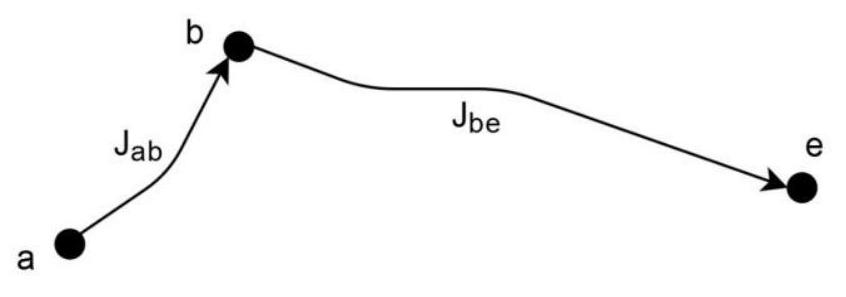
\includegraphics[width=8.5 cm, height=3.0cm]{optimal_path_1.jpg}
    \caption{Optimal Path Problem}
\end{figure}

\noindent If the cost of going $a \rightarrow b$ in Figure 3.28 is expressed as $J_{a b}$ and the cost of going $b \rightarrow e$ is expressed as $J_{b e}$, the optimal cost will be as in equation 3.37.
\begin{subequations}
\begin{align}
   J_{a e}^{*}=J_{a b}+J_{b e}
\end{align}
\end{subequations}
If $a \rightarrow e$ is our optimal cost $J_{a e}^{*}$ then $b \rightarrow e$ must also be optimal. If path $b \rightarrow c \rightarrow e$ is more optimal than path $b \rightarrow e$, a dilemma arises. Mathematically, it is expressed by equation 3.38.
\begin{subequations}
\begin{align}
   J_{b c e}<J_{b e}
\end{align}
\end{subequations}
Equation 3.39 is obtained by substituting equation 3.38 for equation 3.37.
\begin{subequations}
\begin{align}
   J_{a b}+J_{b c e}<J_{a b}+J_{b e}=J_{a e}^{*}
\end{align}
\end{subequations}
As can be seen from Equation 3.39, it creates a situation contrary to the principle of optimality. If $J_{a e}^{*}, a \rightarrow e$ is an optimal path, a more optimal subpath cannot be created. This situation is seen in Figure 3.29.
\begin{figure}[h]
    \centering
    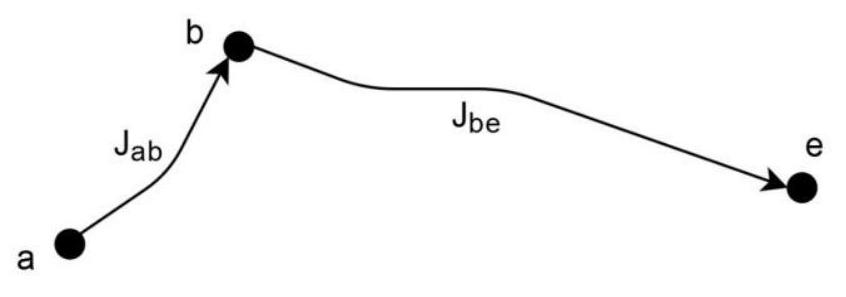
\includegraphics[width=8.5 cm, height=3.0cm]{optimal_path_1.jpg}
    \caption{Optimal Path Problem Contradiction.}
\end{figure}

\noindent The principle of optimality is for discrete time systems, $\pi^{*}=\left\{\pi_{0}^{*}, \pi_{1}^{*}, \ldots, \pi_{N-1}^ {*}\right\}$ should be an array of optimal decisions. Assuming that the $S_{t}$ states are accessible, that is, by constructing a mathematical model, the transition costs of the subproblems based on $t$ from the $S_{t}$ state should be minimal. Thus, the principle of optimality is divided into sub-optimal problems. Dynamic programming is applied in two different ways as forward and backward for the solution of sub-optimal problems. Dynamic programming is called deterministic dynamic programming if the transitions between states are deterministic, and stochastic dynamic programming if the transitions between states are random. Dynamic programming is used in sequential decision making problems and is used in model-based RL problems. In order to solve the Markov decision process with dynamic programming, it is necessary to know the state transition matrix [19].

\subsection{Bellman Equation}.
In model-free RL, the environment of the agent is modeled by the Markov decision process. Our aim is to calculate the optimal policy or optimal value functions, which are the solution of the Markov decision process. The optimal value function is expressed as $V_{*}(s)$ by equation 3.25. In order for the artificial agent to calculate the optimal value expression, it must generate the values of each state. This situation is as in equation 3.40.
\begin{subequations}
\begin{align}
   V(s)=E\left[G_{t} \mid S_{t}=s\right]
\end{align}
\end{subequations}
In equation 3.40 $G_{t}=R_{t+1}+\gamma R_{t+2}+\ldots=\sum_{k=0}^{\infty} \gamma^{k} R_{t +k+1}$ denotes future reward values. Bellman's equation, which creates an iterative approach in the calculation of equation 3.40, is as in equation 3.41.
\begin{subequations}
\begin{align}
   &V(s)=E\left[G_{t} \mid S_{t}=s\right], \\
    &=E\left[R_{t+1}+\gamma R_{t+2}+\gamma^{2} R_{t+3}+\ldots \mid S_{t}=s\right], \\
    &=E\left[R_{t+1}+\gamma\left(R_{t+2}+\gamma R_{t+3}+\ldots\right) \mid S_{t}=s\right], \\
    &=E\left[R_{t+1}+\gamma G_{t+1} \mid S_{t}=s\right], \\
    &=E\left[R_{t+1}+\gamma V\left(S_{t+1}\right) \mid S_{t}=s\right]
\end{align}
\end{subequations}
Equation 3.41 expresses the state value function. The expected value expression of Equation 3.41 $E[ . ]$ is expressed by the next states. $E\left[R_{t+1}\right] \rightarrow R_{t+1}$, so the expected value is calculated only with term $E\left[\gamma V\left(S_{t+1}\right)\right]$ on the right side of the equation. Equation 3.42 is obtained iteratively by adding the expected value, namely the average calculation, to equation 3.41. This equation is referred to as the Bellman equation.
\begin{subequations}
\begin{align}
   V(s)=R_{s}+\gamma \sum_{s^{\prime} \in S} P_{s s^{\prime}} V(s)
\end{align}
\end{subequations}
Equation 3.42 writes a state-value function with the future reduced reward values of each state. The Bellman equation is expressed with the action value function as in equation 3.43.
\begin{subequations}
\begin{align}
   q(s, a)=R_{s}^{a}+\gamma \sum_{s^{\prime} \in S} P_{s s^{\prime}}^{a} q(s, a)
\end{align}
\end{subequations}
Thanks to equation 3.43 and equation 3.42, value-based RL approach can be calculated iteratively in the environment modeled by Markov decision process. In the model-independent RL approach, the $P_{s s^{\prime}}, P_{s s^{\prime}}^{a}$ state transition probabilities matrix is unknown. In this case, the artificial agent cannot form the solution of the Markov decision process. Equation 3.43 and equation 3.42 can be approximated by using the temporal difference or the fitted carousel approximation. In this thesis, iterative solutions of equation 3.42 and equation 3.43 will be examined with temporal difference algorithms [21].

\subsection{Policy Based Reinforcement Learning}
The policy-based solution of RL aims to find a policy instead of establishing the values of the states as an alternative to the value-based approach to MDP. In the previous section, state-value and action-value functions were examined for the solution of MDP. In these approaches, $V_{\pi}(s), q_{\pi}(s, a)$ functions were updated with the rewards of the artificial agent in the environment. An agent-generated policy for the update process was not reviewed. For example, a policy selection was made that maximizes the status values. For a deterministic policy, this is expressed in equation 3.30. The policy-based approach proposed for the solution of RL enables the artificial agent to develop a behavior in the environment. The behavior of the agent can be deterministic or stochastic. A deterministic policy is shown in equation 3.44.
\begin{subequations}
\begin{align}
   \pi_{\theta}(s)=\max _{a \in A} \theta(s, a)
\end{align}
\end{subequations}
Similar to equation 3.44, if the policy is stochastic, the policy expressed by equation 3.45 can be formed.
\begin{subequations}
\begin{align}
   \pi_{\theta}(a \mid s)=\frac{\exp \theta(s, a)}{\sum_{a^{\prime} \in A} \exp \theta\left(s, a^{\prime}\right)}
\end{align}
\end{subequations}
The policy created by equations 3.443 and 3.45 is different from the policy expressed by equation 3.30 written for the solution of the Markov decision process. Note that $\theta$ is an arbitrary parameter here. The value of a policy is the expected value of future rewards reduced by equation 3.22. This situation is seen in equation 3.46.
\begin{subequations}
\begin{align}
   V_{\pi}(s)=E_{\pi}\left[R_{t+1}+\gamma V_{\pi}\left(S_{t+1}\right) \mid S_{t}=s\right]
\end{align}
\end{subequations}
The optimization problem created for the policy-based solution of RL is expressed as in equation 3.47 by expanding equation 3.46.
\begin{subequations}
\begin{align}
   V_{\theta}(s)=E\left[\sum_{t=1}^{\infty} \gamma^{t} r_{t} \mid s_{t+1} \sim P\left(s^{\prime} \mid s_{t}, \pi_{\theta}\left(s_{t}\right)\right), s_{1}=s\right]
\end{align}
\end{subequations}
As expressed in Equation 3.47, policy can be calculated over a long horizon. The analytical gradient $\nabla_{\theta} V_{\theta}(s)$ of the policy value expressed in equation 3.47 is unknown. An approximate solution of $\nabla_{\theta} V_{\theta}(s)$ is required to solve the optimization problem. A simple policy search algorithm is shown in Algorithm 3.1.
\newpage
\begin{algorithm}
\caption{Simple Policy Search Algorithm}
\begin{algorithmic}[1]
\State $\theta^{(1)}, \theta^{(2)}, ....., \theta^{(M)}$ $\triangleright$ Add random noise to the parameters for M trials and empirically calculate the reward sum $V^{(i)} = \sum_{t=1}^{T} \gamma ^{t}r_{t}.$
\State $V^{(i)} \approx  f(\theta ^{(i)})$ $\triangleright$ train any parametric machine learning model according to the supervised learning model.
\State $\theta \leftarrow \theta + \alpha \triangledown _{\theta }f(\theta )$ $\triangleright$ update parameters.
\end{algorithmic}
\end{algorithm}

\noindent Apart from the simple policy search algorithm expressed in Algorithm 3.1, another policy search algorithm is the policy gradient and reinforce method. This method forms the basis of many policy-based RL algorithms. The value function of the policy can be expressed as in equation 3.48 to express the trajectory we follow as $\tau=\left(s_{1}, a_{1}, s_{2}, a_{2}, \ldots, s_{T}, a_{T}\right)$ state action pair.
\begin{subequations}
\begin{align}
   V_{\theta}(s)=E[R(\tau) ; \theta]=\int p(\tau ; \theta) R(\tau) d \tau
\end{align}
\end{subequations}
Equation 3.48 needs to be edited to create the reinforce algorithm. This arrangement is first expressed through the gradient calculation of equation 3.48 as in equation 3.49.
\begin{subequations}
\begin{align}
   &\nabla_{\theta} V_{\theta}(s)=\nabla_{\theta} \int p(\tau ; \theta) R(\tau) d \tau, \\
&=\int \nabla_{\theta} p(\tau ; \theta) R(\tau) d \tau, \\
&=\int \frac{p(\tau ; \theta)}{p(\tau ; \theta)} \nabla_{\theta} p(\tau ; \theta) R(\tau) d \tau, \\
&=\int p(\tau ; \theta) \nabla_{\theta} \log p(\tau ; \theta) R(\tau) d \tau, \\
&=E\left[\nabla_{\theta} \log p(\tau ; \theta) R(\tau)\right]
\end{align}
\end{subequations}
With equation 3.49, the gradient of the function $V_{\theta}(s)$ can be calculated $\nabla_{\theta} V_{\theta}(s)$. It should be noted in Equation 3.49 that an expected value calculation is made so that an estimate is made from the sample. The proposed policy gradient and the second adjustment of the reinforcement algorithm for the policy search are done on the equation 3.49. This situation is expressed in equation 3.50.
\begin{subequations}
\begin{align}
   &\nabla_{\theta} \log p(\tau ; \theta)=\nabla_{\theta} \log \left(\prod_{t=1}^{T} p\left(s_{t+1} \mid s_{t}, a_{t}\right) \pi_{\theta}\left(a_{t} \mid s_{t}\right)\right), \\
&=\nabla_{\theta} \sum_{t=1}^{T}\left(\log p\left(s_{t+1} \mid s_{t}, a_{t}\right)\right)+\nabla_{\theta} \log \pi_{\theta}\left(a_{t} \mid s_{t}\right), \\
&=\sum_{t=1}^{T} \nabla_{\theta} \log \pi_{\theta}\left(a_{t} \mid s_{t}\right)
\end{align}
\end{subequations}
The policy optimization algorithm using Equation 3.50 is seen in Algorithm 3.2. Since Equation 3.50 does not depend on gradient transition probabilities, the first part to the right of the equation is zero.
\begin{algorithm}
\caption{Policy Gradient and REINFORCE Algorithm}
\begin{algorithmic}[1]
\State For a stochastic policy $\pi _{\theta}$, construct the $\tau$ trajectory in M steps.
\State Gradient Value $g_{\theta }\leftarrow\frac{1}{M} \left ( \sum_{t=1}^{M}\left ( \sum_{t=1}^{T} \nabla_{\theta} \log \pi_{\theta}\left(a_{t}^{(i)} \mid s_{t}^{(i)}\right) \right ) R(\tau ^{(i)}) \right )$
\State Update parameters. $\theta\leftarrow \theta + \alpha g_{\theta }$
\end{algorithmic}
\end{algorithm}

\noindent The algorithm proposed in Algorithm 3.2 is the calculation of the gradient over the sample and does not calculate the actual gradient value. It should be noted that the sample of the agent in the environment is very good and should determine the policy in the best way. Since there is no information about the environment in the model-independent RL approach, the agent must discover the environment and then use the experiences gained from his discoveries. Value-based or policy-based algorithms need to travel around the environment for a while to gather information. The $\varepsilon-$greedy approach expressed in the previous section is used for RL algorithms with equation 3.51 [22].
\begin{subequations}
\begin{align}
   \pi(s)=\left\{\begin{array}{cc}
\max \hat{Q}(s, a) & 1-\varepsilon \\
\text { random action } & \text { otherwise }
\end{array}\right.
\end{align}
\end{subequations}

\subsection{Value Based Reinforcement Learning}
The Markov decision process provides a mathematical basis for RL. The Markov decision process has been examined in detail in the previous section. The solution of the Markov decision process is obtained by solving the optimal state-value or action-value functions. This situation is expressed in equation 3.52.
\begin{subequations}
\begin{align}
    V_{*}(s)=\max _{a} R_{s}^{a}+\gamma \sum_{s^{\prime} \in S} P_{s s^{\prime}}^{a} V_{*}(s), \\
q_{*}(s, a)=R_{s}^{a}+\gamma \sum_{s^{\prime} \in S} P_{s s^{\prime}}^{a} \max _{a^{\prime}} q_{*}(s, a)
\end{align}
\end{subequations}
The $V_{*}(s)$ in Equation 3.52 expresses the optimal solution of the state-value function and constitutes the solution of the MDP. Similarly, $q_{*}(s, a)$ is an optimal solution of the actionvalue function and is the solution of the MDP. In the approaches expressed by Equation 3.52, it is expressed how it will receive a reward value in the environment modeled with the artificial agent MDP and how it will update the functions according to these reward values. These solution approaches constitute MDP's value-based solutions. The $P_{s s^{\prime}}^{a} R_{S}^{a}$ expressed in Equation 3.52 is unknown. 
\\ \\
Since the state transition matrix and the reward function are not known, the closed form solution of the MDP cannot be calculated. By making observations in its environment, the artificial agent samples the $s_{t+1}$ state from the $P\left(s^{\prime} \mid s_{t}, a_{t}\right)$ distribution function. An approximate calculation is made with these observation values and the reward function written over the states in the $r_{t}$ environment. This situation is expressed in equation 3.53.
\begin{subequations}
\begin{align}
    \hat{V}^{\pi}\left(s_{t}\right)=r_{t}+\gamma \hat{V}^{\pi}\left(s_{t+1}\right)
\end{align}
\end{subequations}
Equation 3.53 values the state $s_{t}$ with the reward at time $t$ and the next $s_{t+1}$ state and a reduction factor updates as in $r_{t}+\gamma \hat{V}^{\pi}
\left(s_{t+1}\right)$. The update in this state affects the state at time $t$ whether the next state value is positive or negative. By updating Equation 3.53, a more effective update rule, Equation 3.53, is obtained.
\begin{subequations}
\begin{align}
    \hat{V}^{\pi}\left(s_{t}\right) &=(1-\alpha) \widehat{V}^{\pi}\left(s_{t}\right)+\alpha\left(r_{t}+\gamma \hat{V}^{\pi}\left(s_{t+1}\right)\right), \\
\hat{V}^{\pi}\left(s_{t}\right) &=\widehat{V}^{\pi}\left(s_{t}\right)+\alpha(r_{t}+\underbrace{\gamma \widehat{V}^{\pi}\left(s_{t+1}\right)-\hat{V}^{\pi}\left(s_{t}\right)}_{\text {Temporal Difference}}),  \alpha<1
\end{align}
\end{subequations}
If we pay attention to Equation 3.54, the update of $\hat{V}^{\pi}\left(s_{t}\right)$ values at time $t$ occurs by adding the temporal difference part in addition to $\hat{V}^{\pi}\left(s_{t}\right)$. In the temporal difference approach, the update will occur depending on the future discounted reward value $\gamma \hat{V}^{\pi}\left(s_{t+1}\right)$ that the agent will receive. The expression $\gamma \hat{V}^{\pi}\left(s_{t+1}\right)-\hat{V}^{\pi}\left(s_{t}\right)$ is the temporal difference is called the future $\widehat{V}^{\pi}\left(s_{t+1}\right)$ and the current $\hat{V}^{\pi} \left(s_{t} \right)$. 
\\ \\
The difference between the predicted value in the future and the present value indicates how well a decision we made. Thus, the reward values obtained by the agent at the time $t$ will be updated over equation 3.54 more successfully than equation 3.53. The reason why the update in equation 3.53 fails much more than in equation 3.54 is because we are updating with the current state reward and the predicted future reward. In equation 3.54, while the current state value is updated, in addition to the current state value, it is updated with the temporal difference that expresses how right decisions we make in the future. Equation 3.54 provides the solution of the model-independent RL approach with the temporal difference approach. The temporal difference approach is applied to the action-value and state-value approaches. The temporal difference algorithm is expressed in Algorithm 3.3.
\begin{algorithm}
\caption{Temporal Difference Algorithm}
\begin{algorithmic}[1]
\State  $ \hat{V}^{\pi }(s) = 0, \forall s \in S $ $\triangleright$ Algorithm initialization parameter.
\For{t = 1, T}
\State $\; \; s_{t} , r_{t}$ $\triangleright$ Observe states and reward values
\State $\; \; a = \pi (s)$ $\triangleright$ Apply an action with a specific policy.
\State $\; \; s_{t+1}$ $\triangleright$ Observe the next state.
\State $\; \; \hat{V}^{\pi}\left(s_{t}\right) =\widehat{V}^{\pi}\left(s_{t}\right)+\alpha(r_{t}+\gamma \widehat{V}^{\pi}\left(s_{t+1}\right)-\hat{V}^{\pi}\left(s_{t}\right))$ $\triangleright$ with Temporal Difference
make an update.
\EndFor
\end{algorithmic}
\end{algorithm}

\noindent The temporal difference algorithm allows us to approximate $\hat{V}^{\pi}\left(s_{t}\right) \approx V^{\pi}\left(s_{t}\right)$ without generating the MDP [22].

\subsection{Q Learning Algorithm}
The Q learning algorithm is an action-value-based algorithm together with the temporal difference algorithm and is a off policy. As it will be remembered, in the closed policy approach, the policy value followed by the agent is not updated. The Q learning algorithm is similar to the value-based approach. As an alternative to the value-based approach, the Q learning algorithm is expressed over actions and states as in equation 3.55.
\begin{subequations}
\begin{align}
    Q^{\pi}(s, a)=R(s)+\gamma \sum_{s^{\prime} \in S} P\left(s^{\prime} \mid s, a\right) Q^{\pi}\left(s^{\prime}, \pi\left(s^{\prime}\right)\right)
\end{align}
\end{subequations}
The Q learning algorithm, which is a value-based solution algorithm, is as seen in equation 3.55. In the equation, the policy followed by the agent is expressed by $\pi\left(s^{\prime}\right)$. The optimal solution of equation 3.55 is as in equation 3.56.
\begin{subequations}
\begin{align}
    Q^{*}(s, a)=R(s)+\gamma \sum_{s^{\prime} \in S} P\left(s^{\prime} \mid s, a\right) \max _{a \in A} Q^{*}\left(s^{\prime}, a^{\prime}\right)
\end{align}
\end{subequations}
In Equation 3.56, the agent's policy can be created as the action selection that produces the maximum value over $\pi\left(s^{\prime}\right) \mathrm{Q}$ values. Equation 3.56 forms the basis of the Q learning algorithm. Thus, the agent is expressed in the MDP with the state and action value function. In Equation 3.56, where $P\left(s^{\prime} \mid s, a\right), R(s)$ is unknown, that is, the MDP is not exactly known, if we only have the measurements at time $t$, the solution of the MDP In order to find the optimal state action value function $Q^{*}(s, a)$, equation 3.56 needs to be updated with the temporal difference approximation. This situation is expressed in equation 3.57.
\begin{subequations}
\begin{align}
    &\widehat{Q}^{*}(s, a)=(1-\alpha) \hat{Q}^{*}(s, a)+\alpha\left(r+\gamma \max _{a \in A} \hat{Q}^{*}\left(s^{\prime}, a^{\prime}\right)\right), \\
&\hat{Q}^{*}(s, a)=\widehat{Q}^{*}(s, a)+\alpha(r+\underbrace{\gamma \max _{a \in A} \widehat{Q}^{*}\left(s^{\prime}, a^{\prime}\right)-\widehat{Q}^{*}(s, a)}_{\text {Temporal Difference }})
\end{align}
\end{subequations}
The Q learning algorithm created with Equation 3.57 converges to its real values $Q^{*}(s, a) \approx \widehat{Q}^{*}(s, a)$ by applying enough states and actions in the environment where the agent is located. One advantage of learning Q is that we can learn optimal policy values by making action choices without MDP in our hands. This situation is expressed in equation 3.58.
\begin{subequations}
\begin{align}
    \pi^{\ast } (s) = \underset{a \in A}{\arg \max } \,\hat{Q}^{\ast } (s,a)
\end{align}
\end{subequations}
Q learning algorithm expressed by Equation 3.57 is seen in Algorithm 3.4.
\begin{algorithm}
\caption{Q Learning Algorithm}
\begin{algorithmic}[1]
\State $\alpha \in (0,1], \gamma$ $\triangleright$ Set learning rate and discount rate parameter
\State $\varepsilon > 0$ $\triangleright$ Epsilon too small number for random action selection
\State $Q(s,a) = 0s \in S, a \in A$ $\triangleright$ The start of the Q value is zero for actions and states.
\State How many Episode the algorithm will run?
\State How many steps (T) will the algorithm take in each section?
\For{e = 1, Episode}
    \State s $\triangleright$ initilization state
    \For{t = 1, T}
        \State Random action with $\varepsilon$ possibilities
        \State  $a = \max_{a \in A} Q(s,a)$ action with $1 - \varepsilon$ possibilities
        \State Apply a action, save the next state and reward $(s^{\prime}, r)$ 
        \State $\hat{Q}^{*}(s, a)=\widehat{Q}^{*}(s, a)+\alpha(r+\gamma \max _{a \in A} \widehat{Q}^{*}\left(s^{\prime}, a^{\prime}\right)-\widehat{Q}^{*}(s, a))$ $\triangleright$ update the Q table
        \State s $\leftarrow s^{\prime}$
        \EndFor
        \EndFor
\end{algorithmic}
\end{algorithm}

\noindent Q learning algorithm expressed in Algorithm 3.4 is applicable for finite discrete state and action pair. Since states and actions are in continuous time in control theory, Q learning algorithm is not applied for steady state and action pair [22].

\subsection{Sarsa Algorithm}
As we discussed, Q learning algorithm is a  off-policy algorithm, the policy value does not change and follows a fixed policy as in equation 3.51. The Q learning algorithm approximates the Markov decision process over state-action values under a fixed policy. The Sarsa algorithm is very similar to the Q learning algorithm but it is on-policy. Mathematically, the Sarsa algorithm is expressed as in equation 3.59.
\begin{subequations}
\begin{align}
    &\widehat{Q}^{\pi}(s, a)=(1-\alpha) \hat{Q}^{\pi}(s, a)+\alpha\left(r+\gamma \hat{Q}^{\pi}\left(s^{\prime}, \pi(s^{\prime}) \right)\right), \\
&\hat{Q}^{\pi}(s, a)=\widehat{Q}^{\pi}(s, a)+\alpha(r+\underbrace{\gamma \widehat{Q}^{\pi}\left(s^{\prime}, \pi(s^{\prime}\right))-\widehat{Q}^{\pi}(s, a)}_{\text {Temporal Difference }})
\end{align}
\end{subequations}
Paying attention to Equation 3.59, the Q values are updated over a certain policy $\pi (s)$. The policy, which is fixed in the Q learning algorithm, is parametric in the Sarsa algorithm. This approach makes the Sarsa algorithm an open policy algorithm. While updating is made over the policy values followed in the previous step in the Q learning algorithm, the next Q values in the Sarsa learning algorithm are calculated and updated over a certain policy. The new Q values used for updating in Q learning are calculated with a greedy approach with $\max_{a^\prime \in A} Q(s^\prime, a^\prime)$. In the Sarsa learning algorithm, this is calculated by following a policy $\hat{Q}^{\pi }(s^\prime,\pi(s^\prime))$ for new Q values. This approach is the main difference between Q learning and Sarsa learning. The Sarsa algorithm is expressed in Algorithm 3.5.
\begin{algorithm}
\caption{Sarsa Algorithm}
\begin{algorithmic}[1]
\State $\alpha \in (0,1], \gamma$ $\triangleright$ Set learning rate and discount rate parameter
\State $\varepsilon > 0$ $\triangleright$ Epsilon too small number for random action selection
\State $Q(s,a) = 0s \in S, a \in A$ $\triangleright$ The start of the Q value is zero for actions and states.
\State How many Episode the algorithm will run?
\State How many steps (T) will the algorithm take in each section?
\For{e = 1, Episode}
    \State s $\triangleright$ initilization state
    \State We determine the (a) action that the agent should take for the (s) state
    \For{t = 1, T}
        \State Apply a action, save the next state and reward $(s^{\prime}, r)$ 
        \State We determine the $(a^\prime)$ action that the agent should take for the $(s^\prime)$ state
        \State $Q(s, a)=Q(s, a)+\alpha(r+\gamma Q\left(s^{\prime}, a^{\prime}\right)-Q(s, a))$ $\triangleright$ update the Q table
        \State s $\leftarrow s^{\prime}$ , a $\leftarrow a^{\prime}$
    \EndFor
\EndFor
\end{algorithmic}
\end{algorithm}

\noindent The main difference between Sarsa and Q learning is that learning Q tries to create the optimal path whereas Sarsa learning aims to create the optimal path in the safest way. While Q learning only acts on maximum values, Sarsa learning algorithm makes maximum values by updating future states and actions. Thus, Sarsa learning calculates the next decisions based on current policy. In Q learning, the next decisions are calculated only on the maximum values [19].

\section{Deep Neural Networks}
AI is a critical field of science in today's technology, both in terms of its applications and in creating devices that can think. AI models machines by imitating human brains, mentality, learning, and decision-making abilities. DL is a sub-field of ML that uses multi-layer artificial neural networks in areas such as object recognition, speech recognition, and natural language processing. Unlike traditional ML techniques, DL can automatically learn from symbols in photos, movies, audio, and texts [26]. This chapter examines the logic and concepts of deep neural networks, which are the core of DL.

\subsection{Building Units}
We mentioned that DL is an AI method that uses multi-layer artificial neural networks in many areas, and considered as sub-field of ML. Especially recently, DL has been used frequently in the field of RL. This combination also brought solutions to many problems. Unlike traditional ML methods, DL can learn automatically by feeding on data from images, videos, sounds and texts instead of learning with coded rules. Because they are flexible, they can also learn from raw image or text data, and their prediction accuracy can increase with the size of the data. However, DL performs the learning process through examples [27]. For a problem that the machine is asked to solve, instead of reaching a solution using rule sets, it is sufficient to give a model that allows it to solve the problem by evaluating the examples. In order to correct the error in the solution of the problem, a simple command list is given and the machine is expected to perform the learning process. Model selection is effective in solving the problem. The model to be determined in accordance with the problem will contribute more to the solution of the problem. The concept of DL was first introduced by [110], when it was suggested that multi-layer artificial neural networks could be trained more efficiently. These networks are also called deep neural networks.
\\ \\
Today, machines that are designed and coded in many areas or software are installed are expected to facilitate human life. However, the question of how to do this with the limited memory of machines consisting of certain code blocks is beginning to find its answer with new studies on machines. The era of machines that are manually coded by humans or that only perform certain functions ends with the emergence of the concept of AI. 
\\ \\
So, what is AI? How could machines be more intelligent? AI is defined as machines imitating the learning process in humans. Considering that the human brain performs the learning process, the information processing capacity of the brain has been examined (Figure 3.30). In order for machines to learn like humans, the brain tries to imitate nerve cells called neurons, which are active in the learning process and determine the brain's capacity to process information.
\begin{figure}[h]
    \centering
    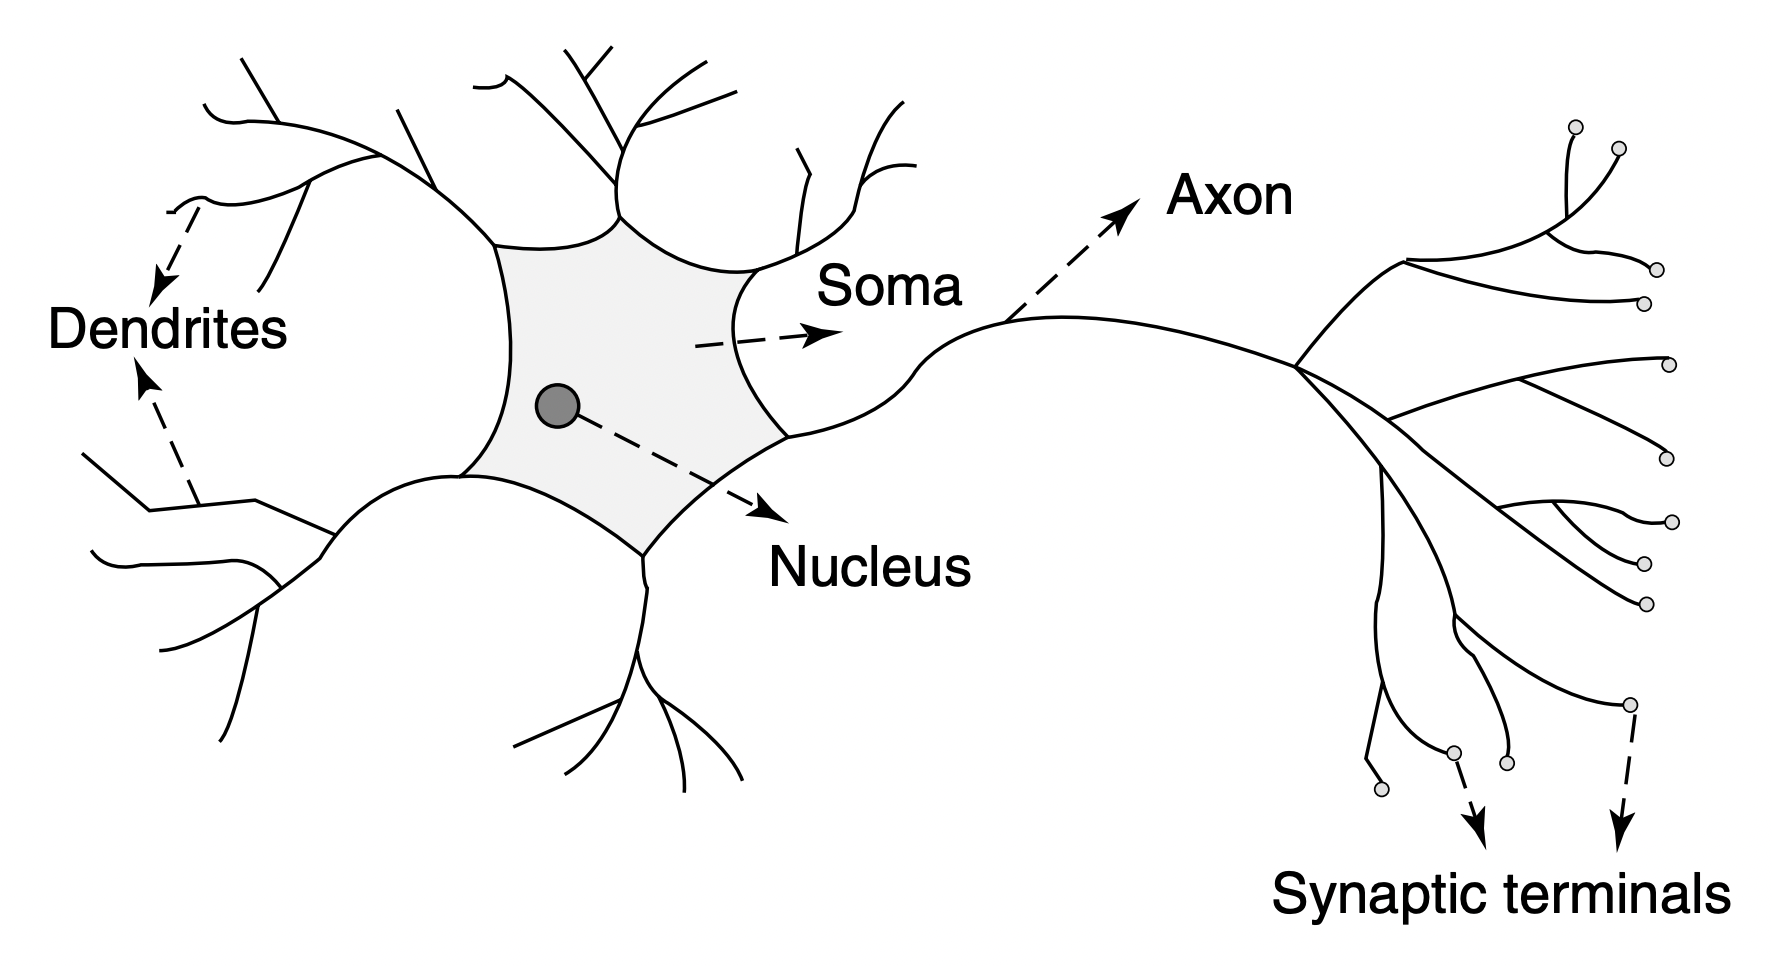
\includegraphics[width=7.4cm, height=3.4cm]{neuron.png}
    \caption{The structure of a neuron [28]}
\end{figure}

\noindent There are dendrite, cell nucleus, cell body, axon, myelin sheath, node of Ranvier, Schwann cell and axon terminals in the neuron. As a result of imitating neurons, which are nerve cells in humans, the concept of artificial neurons was introduced.

\subsubsection{Artificial Neuron}
The neuron, which forms the basic structure of the neural network, is the basic element of our brain (Figure 3.31). When new information is received, this information is processed and then converted to output. In a neural network, an input to a neuron is received, processed, and produces an output or result output that is sent to other neurons for further processing.
\begin{figure}[h]
    \centering
    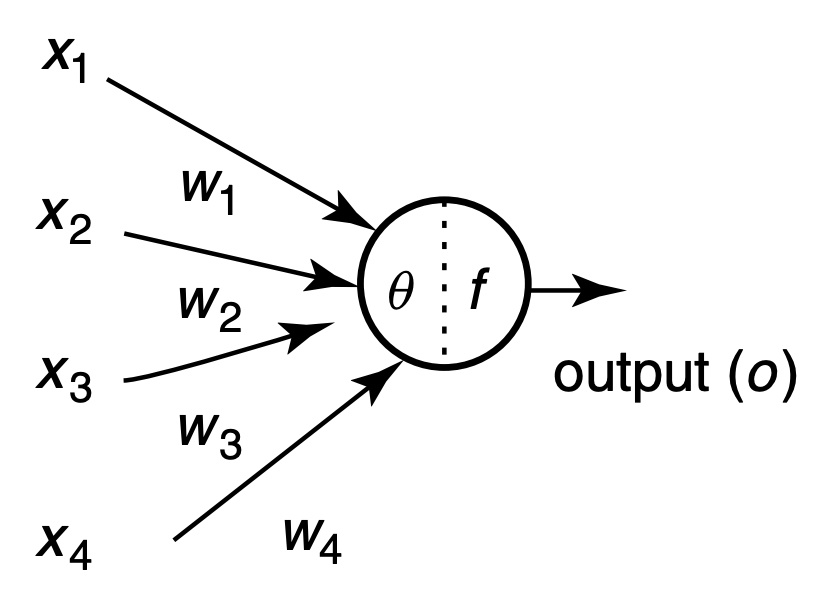
\includegraphics[width=8.1cm, height=6.1cm]{art_neuron.png}
    \caption{Artificial neuron [28]}
\end{figure}

\subsubsection{Weights}
When the input arrives at the neuron, it is multiplied by a weight. In a two-input neuron, each neuron input has a weight assigned to that input. These randomly initialized weights are updated during the training of the model. A higher weight value is given to the inputs that are considered to be more important after the training by the neural network. However, it may be concluded that an input or feature that is given a zero weight value by the neural network is unimportant. Assuming an input \textbf{$x$} is associated with the weight $w_1$, the input after passing through the node is expressed as \textbf{$x$} $*$ $w_1$

\subsubsection{Bias}
The additional linear component applied to the input, different from the weight applied, is called bias. This bias value is the result of multiplying the input by the weight, which is defined as the input, is added as the basis for changing the range of the input with the weight coefficient. As a result of adding the bias value, the input is expressed as \textbf{$x$} $*$ $w_1$+bias (Figure 3.32). This input is the last linear component of your transformation.

\subsubsection{Activation Functions}
The implementation of the activation function, which converts the input signals to the output signals, to the linear combination is performed by applying the nonlinear function after the linear component is applied to the input (Figure 3.32). After applying the activation function \textbf{$f()$}, the output will be \textbf{$f(x_1*w_1+b)$}. The weights are first multiplied by their corresponding input and then the bias is added to the product result. 
\\ \\
If the expression formed as a result of adding the bias value to the product of the input sums corresponding to the weight sums is accepted as u: 
\begin{center}
    $u = \sum w * x + b $
\end{center}

\noindent As a result of applying the activation function to u, f(u) is formed and the final output obtained from the neuron is expressed as $y_i=f(u)$.
\begin{figure}[h]
    \centering
    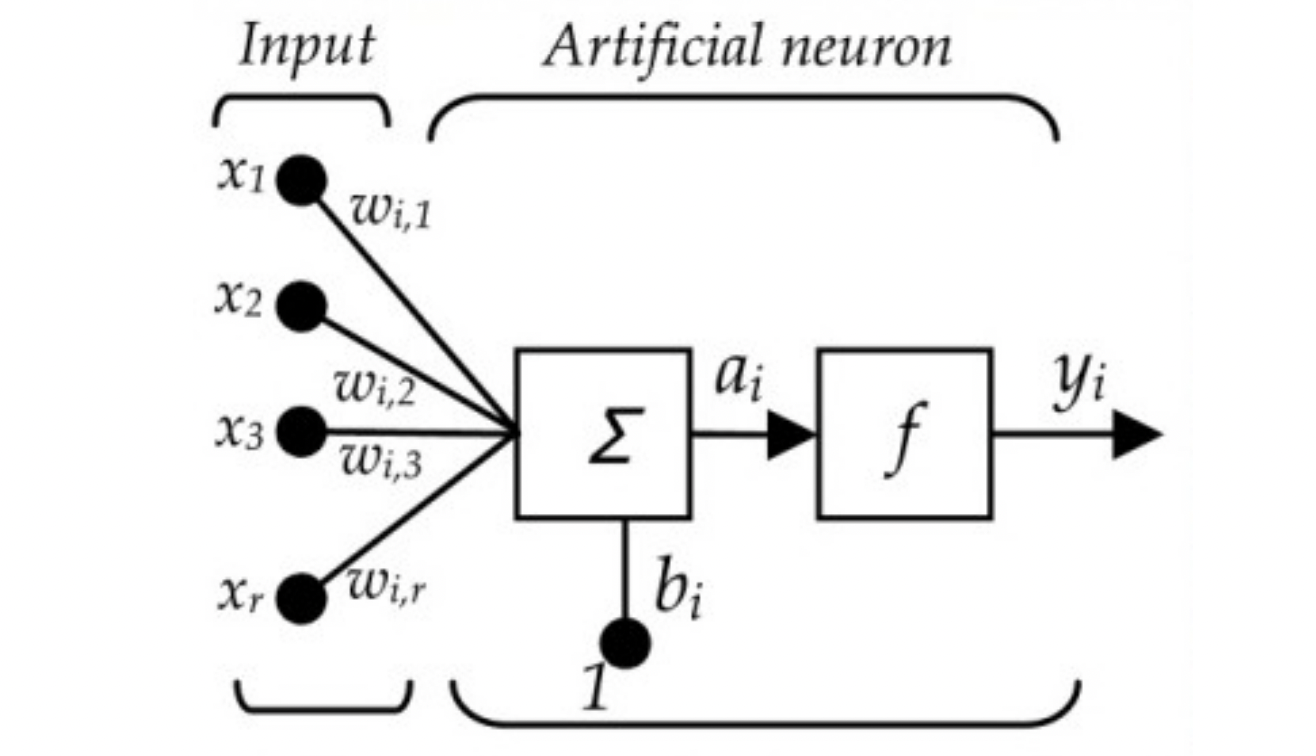
\includegraphics[width=13cm, height=7.5cm]{weight-bias.png}
    \caption{Weights, biases and activation function in an artificial neuron [29]}
\end{figure}

\noindent The most commonly used activation functions are sigmoid, ReLU, tanh and linear. You can see the comparison of the activation functions in Figure 3.33.
\begin{figure}[h]
    \centering
    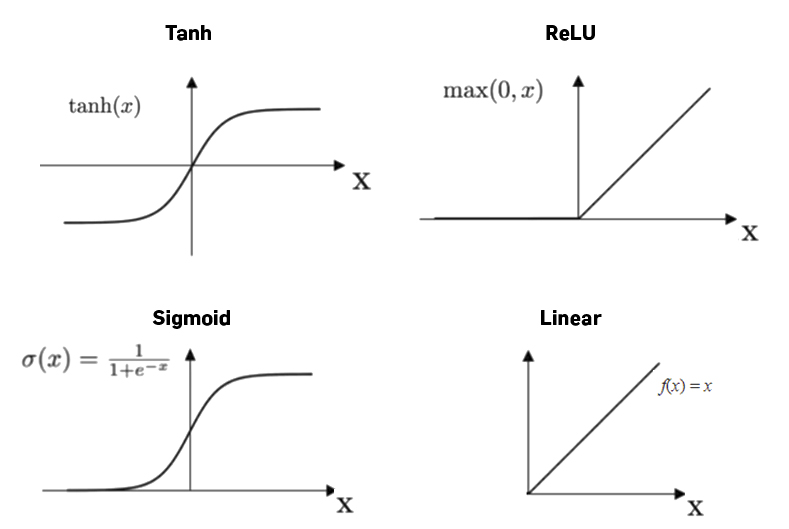
\includegraphics[width=10.5cm, height=7.0cm]{activation-functions.jpeg}
    \caption{Different activation function types [30]}
\end{figure}

\subsection{Forward and Backward Propagation}
Neural networks form the basis of DL. The purpose of these neural networks is to determine the approximation of the function of an unknown function. Neural networks are made up of neurons that are interconnected. It has bias and weight values that are updated depending on the error value during the training of each neuron network. The function of the activation function ensures that the linear combination that produces the output reveals the nonlinear transformation. The combinations of the operated neurons give the output of the network.

\subsubsection{Input, output and hidden layers}
Basically the first layer of the network and the input layer of the network is the input layer. The output layer is the last layer of the network that produces the output of the network. Process layers in the network are also hidden layers in the network. Hidden layers are layers that perform certain tasks on incoming data and transfer the output created as a result of these tasks to the next layer (Figure 3.34). The middle layers are hidden, while the input and output layers are visible.
\begin{figure}[h]
    \centering
    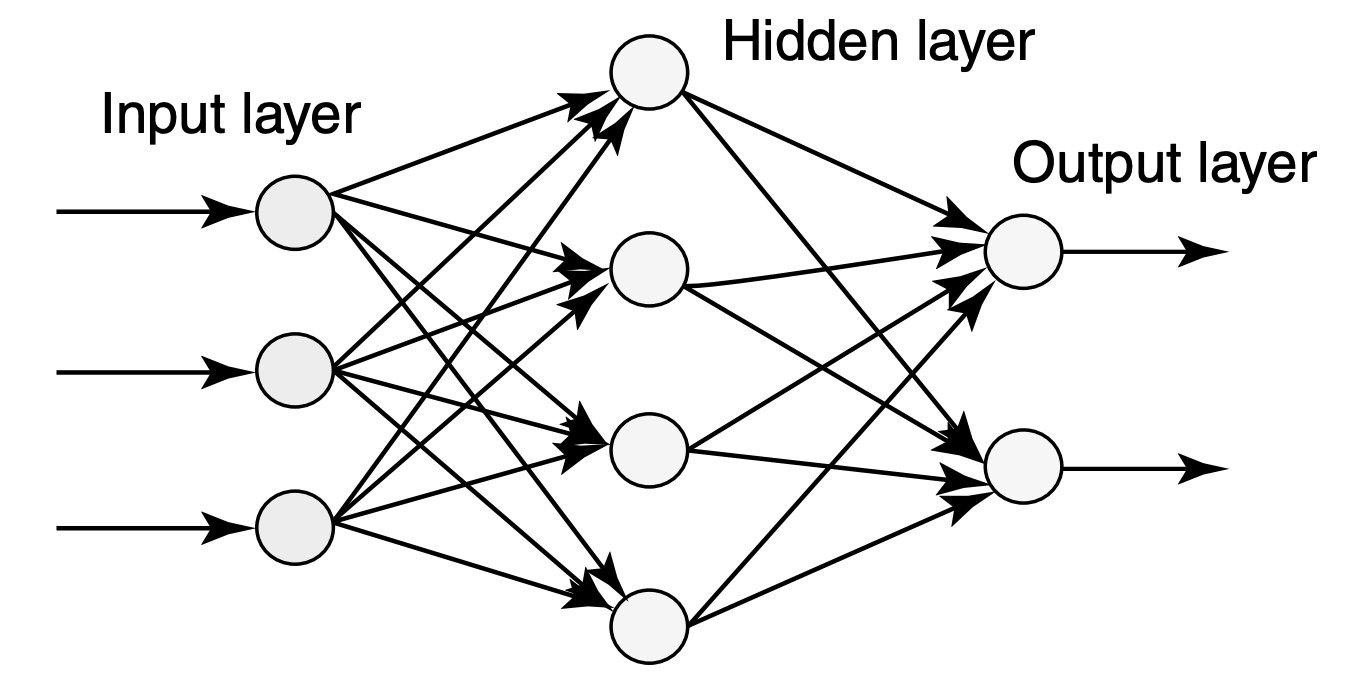
\includegraphics[width=13.6cm, height=6.8cm]{MLP.png}
    \caption{Layers of an artificial neural network [28]}
\end{figure}

\subsubsection{Multi Layer Perception (MLP)}
Stacks of neurons, which are composed of more than one neuron, are employed to produce the desired outputs because a single neuron is insufficient to carry out complex tasks. The basic building blocks of a network are an input layer, a hidden layer, and an output layer. These networks, also known as fully connected networks, have several neurons in each layer, and each layer's neurons are linked to the layer above it. (Figure 3.35)
\begin{figure}[h]
    \centering
    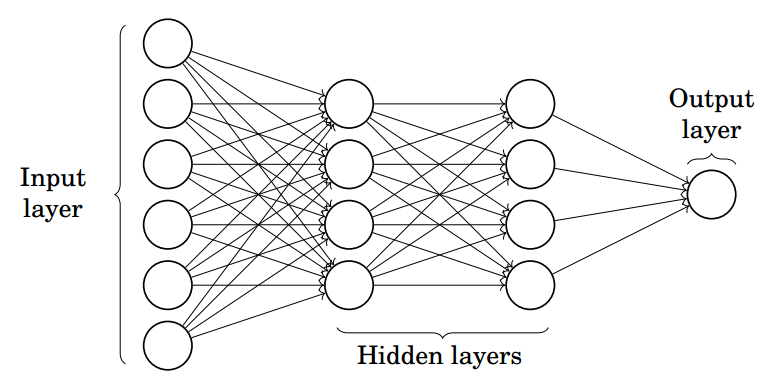
\includegraphics[width=7.7cm, height=4.0cm]{multilayer-perceptron.png}
    \caption{Example MLP [31]}
\end{figure}

\subsubsection{Forward Propagation}
It is forward propagation, which means that the input data is transferred from the input layer to the hidden layer and then to the output layer. In the forward propagation movement, information travels only in one direction and forward. The input layer provides the input for the hidden layers, the information transferred to the hidden layer is transferred to the output layer to produce output, and the process is terminated by producing output in the output layer. There is no backward movement in this structure.

\subsubsection{Loss Function}
The purpose of the created network is to try to estimate the outputs closest to the real values. The truth value of the network is calculated using the cost or loss function. The cost or loss function tries to penalize the network if there is an error in estimating its true values. The purpose of running the network is to increase the accuracy of the estimation, reduce the error and minimize the cost function. The network with the lowest cost function value generates the optimized outputs. m is the number of trained inputs; where a is the estimated value and y is the actual value; If cost function is wanted to be defined with mean square error, this function is expressed as:
\begin{center}
    $C = \frac{1}{m} \sum (y - a)^{2}$
\end{center}
The error criteria of the network models, which are frequently used in the calculation of the loss function, are included in Table 3.4.
\\ \\
\begin{table}[h!]
\centering
\begin{tabular}{||c c||} 
 \hline \hline
 \textbf{Task} & \textbf{Loss Function} \\ [0.5ex] 
    \hline\hline
    \multicolumn{1}{|l|}{Regression} & \multicolumn{1}{l|}{Mean Squared Error} \\ \hline
    \multicolumn{1}{|l|}{Regression} & \multicolumn{1}{l|}{Mean Absolute Error} \\ \hline
    \multicolumn{1}{|l|}{Classification} & \multicolumn{1}{l|}{Binary Crossentropy} \\ \hline
    \multicolumn{1}{|l|}{Classification} & \multicolumn{1}{l|}{Categorical Crossentropy} \\ \hline
    \hline
\end{tabular}
\caption{Some of the Common Loss Functions}
\end{table}

\subsubsection{Gradient Descent}
Gradient descent algorithm is used to minimize the cost (Figure 3.36). This algorithm, to be expressed intuitively, is the least inclined movement that occurs in small steps in climbing a hill and descending from a hill. This ensures that the minimum cost point is achieved. To mathematically find the local minimum of a function, one must proceed according to the negative slope of the function.
\begin{figure}[h]
    \centering
    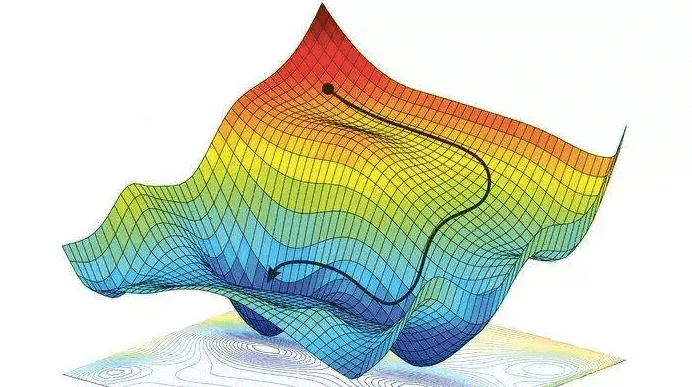
\includegraphics[width=7.0cm, height=4.0cm]{GDescent.png}
    \caption{Graph of gradient descent}
\end{figure}

\subsubsection{Learning Rate}
The amount of minimization obtained in each iteration, which is done to minimize the loss function, is expressed as the learning rate. However, the rate obtained by reducing the cost function to its lowest level is called the learning rate (Figure 3.37). The learning rate should be chosen carefully in order to obtain the most appropriate result in solving the problem. Otherwise, the optimal solution may not be obtained and it may take forever for the network to approach the optimal solution.

\begin{figure}[h]
    \centering
    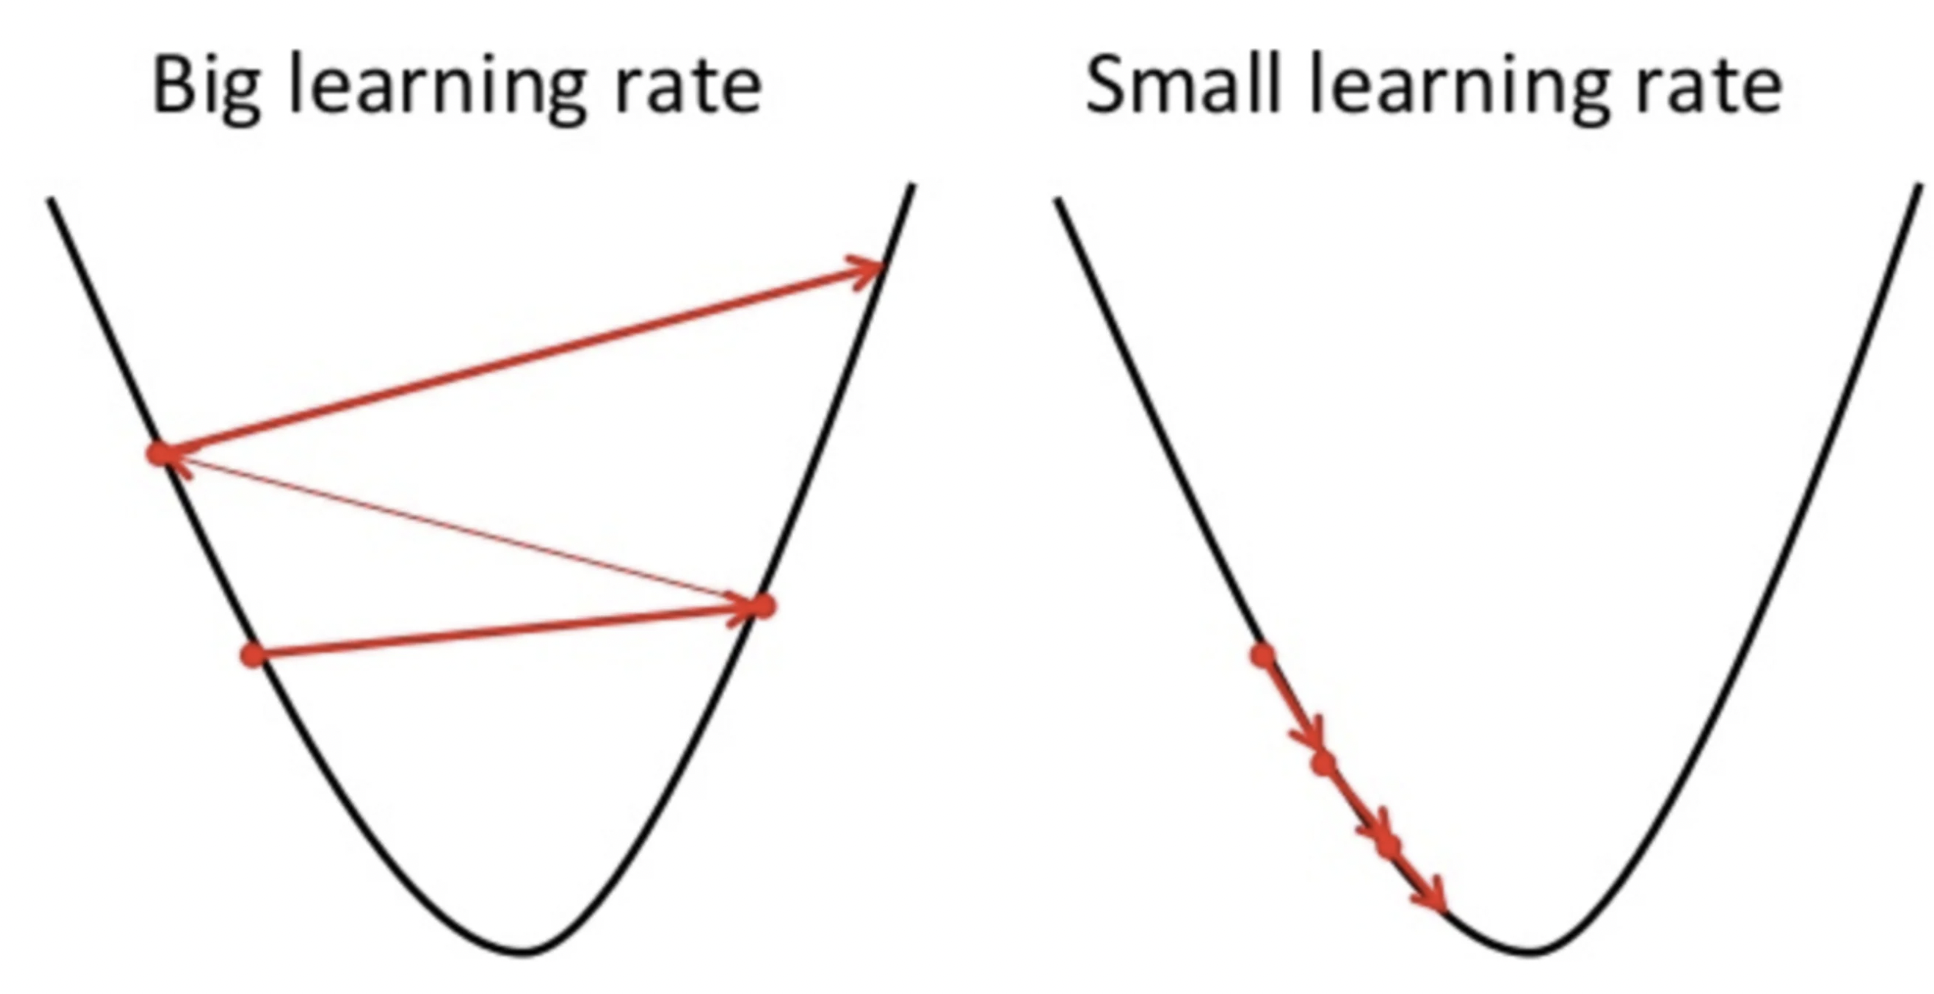
\includegraphics[width=9.7cm, height=5.0cm]{Learning_rate.png}
    \caption{Choosing a learning rate [32]}
\end{figure}

\subsubsection{Backpropagation}
When the neural network is defined, random weight and bias values are assigned to the nodes. The error of the network can be calculated for the output obtained with a single iteration. The resulting error value, along with the slope of the cost function, is fed back to the network so that the weights of the network can be updated. These weights are updated to minimize the error in subsequent iterations. Updating the weights using the slope of the cost function is expressed as back propagation. In back propagation, where the motion of the network is backward, the error along with the slope is transferred backwards from the output layer to the hidden layers, so that the weights are updated.

\subsubsection{Batch}
The inputs are split into independently sized heaps of equal size rather than being sent all at once, and the network is trained as a result. The model created by feeding the inputs from the entire dataset to the network at once is less common than the network model created by training the data as heaps.

\subsubsection{Epoch Numbers}
A single forward and backward propagation training iteration that includes all input data. One epoch number is the total number of iterations produced by training the data once. You can choose to train the network using the epoch number. The accuracy of the network can be increased by selecting more number of repetitions. The network will eventually converge, but it will take time. The network may overfit if the epoch repeats are not carefully chosen or are chosen in excess. 

\subsubsection{Regularization}
ML uses the regularization technique to address the issue of over-fitting in statistical models. To make the network more generalizable to new data, regularization must be introduced. L1 or L2 regularization is the traditional method for addressing the issue of over-fitting. The key component of this approach is the addition of a specific penalty term for weights, $w$, to the loss function. Dropout is a different method that performs better than standard regularization and aids in avoiding the issue of over-fitting.

\subsubsection{Dropout}
It is the term used to describe the regularization method used to stop the network from becoming over-fitted. During training, it is the randomization of a specific number of neurons in the hidden layers (Figure 3.38). Different neural network architectures made up of various neuronal combinations emerge as a result of training. This method is referred to as an aggregation method because it combines the output from various networks to create the final output.
\begin{figure}[h]
    \centering
    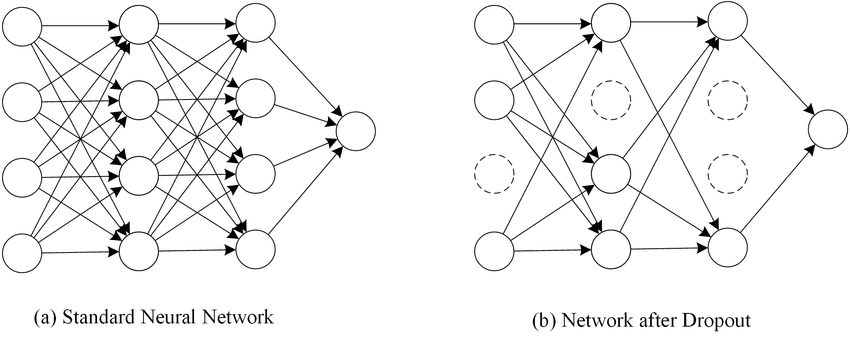
\includegraphics[width=12.5cm, height=5.0cm]{Drop.png}
    \caption{Representaton of dropout in artificial neural network. [33]}
\end{figure}

\subsubsection{Batch Normalization}
It is the process of creating certain checkpoints to ensure that the data distribution is the same as the next layer. The weights in the training of the net change with each step of the downhill. These changes determine how the data will be sent to the next layer. The data is obviously normalized before being sent to the next layer. Because the next layer expects a data stack similar to the distribution sent to this layer before

\section{Deep Reinforcement Learning}
Q learning and Sarsa learning algorithms expressed in chapter 3 are called tabular methods in the literature. These methods are applicable for discrete state and action space and small state space. In real life, the state space and control signal of the control problem are expressed in continuous time and state space is can be very big. In the continuum robot control problem, derivative values of curvature, which is our control sign, are defined in the space of real numbers and take infinite values. 
\\ \\
As a practical application in RL, Q learning and Sarsa learning algorithms can be applied by discretizing continuous state and action spaces, but in practice, the errors that will occur due to discretization pose a problem in control applications. Another problem of the tabular method of RL is to establish the computational cost. Increasing the size of our discrete state and action space causes computational complexity and computational cost to increase. Deep neural networks used in ML are universal function approximators. deep RL methods have been developed by combining the function approximation feature of deep neural networks with the table method algorithms of RL. With the deep RL algorithm, control problems with continuous states can be solved. In addition, table-based algorithms such as the Q learning algorithm are weak in problems with a very large discrete state space. For this reason, deep RL methods are frequently used in problems with very large and discrete state space. Deep Q learning, which is the most used algorithm of deep RL, will be discussed in the next section.

\subsection{Deep Q-Learning}
Deep Q Learning is a RL algorithm that combine Q Learning algorithm and deep neural networks. This method works with discrete action space. The most important difference is the use of deep neural networks instead of Q-Tables. In Q Learning, the Q-Table is used to keep the Q values, and in which case, which action gives which Q value, we read it from the Q table. Unlike Q Learning, here deep neural networks are used to predict actions. The action with the highest result will be the most logical action. Since artificial neural networks are used in Deep Q-Learning, it is necessary to carefully set values such as hidden layer, loss function, number of neurons, and learning rate. In this algorithm, the action comes to the environment, then the result from the environment is the state, action, reward, and next state values, these values enter the deep neural networks and extract 4 different Q-values. Outputs have the Q values and largest Q-value value is selected as the action value and sent to the environment.
\\ \\
The disadvantage of the algorithm is that in the control problem, our control sign $u_{(t)}$ is a continuous function of time. Our actions $a_{(t)}$, which are the equivalent of our control signal in RL, appear in our control problems as a continuous function of time. Due to the fact that actions take discrete values, the deep Q learning algorithm proposed to solve control problems with RL cannot produce sufficient results. The block diagram of the deep Q learning algorithm is shown in Figure 3.39.
\begin{figure}[h]
    \centering
    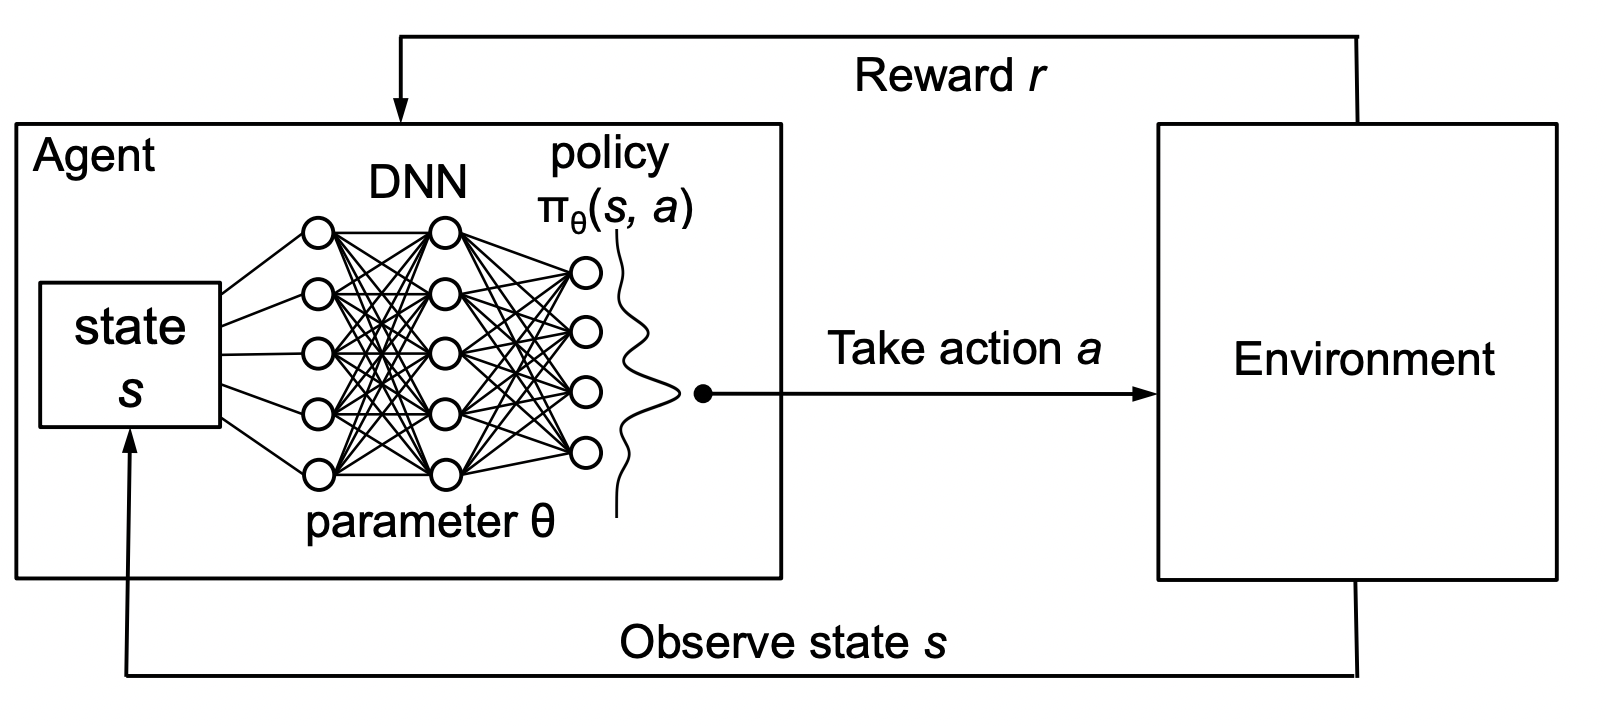
\includegraphics[width=16.0cm, height=7.3cm]{DNN.png}
    \caption{Deep Q Learning working principle [34]}
\end{figure}

\noindent Deep RL algorithm was proposed in 2015. Before moving on to the mathematical foundations of the algorithm, let's examine the Q learning algorithm created with temporal difference. Equation 3.60 shows the Q learning algorithm.
\begin{subequations}
\begin{align}
    Q(s, a)=Q(s, a)+\alpha(r_s +\gamma \max _{a \in A} Q\left(s^{\prime}, a^{\prime}\right)-Q(s, a))
\end{align}
\end{subequations}
Equation 3.60 is updated iteratively. Iterative solution is not possible for steady state values. Function approximation is the basis of the deep Q learning algorithm. Function approximation is created with deep artificial neural networks. This situation is expressed in equation 3.61.
\begin{subequations}
\begin{align}
    Q(s, a: \theta) \approx Q^{*}(s, a)
\end{align}
\end{subequations}
In Equation 3.61, $\theta$ parameter constitutes the parameters of deep artificial neural networks. Let's reconstruct equation 3.60 as in equation 3.62.
\begin{subequations}
\begin{align}
    Q(s, a)=Q(s, a)+\alpha \underbrace{(\underbrace{r_{s}+\gamma \max _{a \in A} Q\left(s^{\prime}, a^{\prime}\right)}_{\text {Target }}-\underbrace{Q(s, a)}_{\text {Prediction }})}_{\text {Cost }}
\end{align}
\end{subequations}
We divide Equation 3.62 into two parts. The first part is the target, the other part is the predicted. This situation is expressed in equation 3.63.
\begin{subequations}
\begin{align}
    &\tilde{y}=r_{s}+\gamma \max _{a \in A} Q\left(s^{\prime}, a^{\prime}: \theta\right), \\
&\hat{y}=Q(s, a: \theta)
\end{align}
\end{subequations}
Using equation 3.63, the cost function is expressed as in equation 3.64.
\begin{subequations}
\begin{align}
    L_{i}\left(\theta_{i}\right)=E_{s, a, r}\left[\left(\tilde{y}-Q\left(s, a, \theta_{i}\right)\right)^{2}\right]
\end{align}
\end{subequations}
Utilizing Equation 3.64, $\theta$ parameters can be found that minimize the cost function $L$ iteratively with the gradient descending algorithm. Equation 3.65 shows the gradient of the cost function.
\begin{subequations}
\begin{align}
    \nabla_{\theta_{i}} L\left(\theta_{i}\right)=E_{s, a, r, s^{\prime}}\left[\left(r+\gamma \max _{a \in A} Q\left(s^{\prime}, a^{\prime}: \theta_{i-1}\right)-Q\left(s, a: \theta_{i}\right)\right) \nabla_{\theta_{i}} Q\left(s, a: \theta_{i}\right)\right]
\end{align}
\end{subequations}
A deep Q learning algorithm can be created using equations 3.64 and 3.65. Deep Q learning algorithm is a model independent approach and is a closed policy algorithm. The $\varepsilon$ - greedy algorithm is used as a fixed policy. Deep Q learning algorithm is seen in Algorithm 3.6 [34]. This algorithm is taken from [104].
\begin{algorithm}
\caption{Deep Q Learning Algorithm}
\begin{algorithmic}[1]
\State $D, C$ $\triangleright$ Create memory space and C update step parameters.
\State $\tilde{Q}(s,a:\theta )$ $\triangleright$ Calculate the prediction value with randomly generated $\theta$ parameters.
\State $\hat{Q}(s,a:\theta )$ $\triangleright$ Calculate the target value with randomly generated $\theta$ parameters.
\For{e = 1, Episode}
    \State $s$ - The initial state of the agent.
    \For{t = 1, T}
        \State Choose random $a_t$ action with probability $\epsilon$.
        \State Choose random $a_t = \underset{a \in A} {\arg \max } Q (s_t, a_t:\theta)$ action with probability $1 - \epsilon$.
        \State Apply $a_t$ action to the system and calculate $r_t, s_{t+1}$ reward and next status.
        \State $D = (s_t, a_t, r_t, s_{t+1})$ $\triangleright$ Save data to memory
        \State $D = (s_j, a_j, r_j, s_{j+1})$ $\triangleright$ Generate random data from memory.
        \State $\tilde{y}=\left\{\begin{array}{cc}
        r_j & t = j + 1 \\
        \tilde{y}=r_{j}+\gamma \max _{a \in A} \hat{Q}\left(s_{j+1}, a: \theta_{t-1}\right) & \text { otherwise }
        \end{array}\right.$
        \State $(\tilde{y}-\hat{Q}(s_j,a_j:\theta_t)^2)$ $\triangleright$ Optimize the cost function with decreasing gradient.
        \State $\hat{Q} = \tilde{Q}$ every $C$ step
    \EndFor
\EndFor
\end{algorithmic}
\end{algorithm}
\newpage
\subsection{Deep Deterministic Policy Gradient}
The DDPG algorithm is created by combining the deterministic policy gradient (DPG) algorithm and the deep Q learning algorithm. Deep Q learning algorithm works on continuous state and discrete action set. 
\\ \\
Many control problems have continuous state and continuous action spaces. Deep Q learning algorithm is a closed policy algorithm and selects actions with $\varepsilon-$greedy approach. This approach is not applied in continuous action space. In order to apply the deep Q learning algorithm to the continuous action space, the action space must be discretized. But discretizing the action space creates many problems. For example, for a 7DoF robot arm, let each joint have appropriate action values $a_{i} \in\{-k, 0, k\}$, so the number of elements in our action space is $3^{7}=2187$. In cases where the resolution of the three elements in the action space is not enough, it is necessary to add more actions and in this case, the 7DoF grows exponentially for a system.
\\ \\
If the action space is too large, it will be impossible for the agent to perform enough actions and discover the environment in which it is located, and the training of the deep $Q$ learning algorithm will not take place. In addition, discretization of the action space causes information loss. The DDPG algorithm solves this problem by learning the policy value with function approximation structures in environments with continuous action space. The DPG algorithm is proposed as the actor-critic algorithm. However, this algorithm has a stability problem. 
\\ \\
A DDPG algorithm is formed by combining the actor-critical algorithm and the deep Q learning algorithm. The performance of the nonlinear function approximator used in the deep $\mathrm{Q}$ learning algorithm has been updated with two innovations to the algorithm. The deep $Q$ learning algorithm provides a more successful convergence thanks to a structure where there is the least correlation between the values recorded in the memory area and learning is provided by sampling from this memory area. A second innovation is $\hat{Q}(s, a: \theta)$ is created and the target model is made and the algorithm is updated accordingly. In Algorithm 3.6, this situation is expressed in the deep Q learning algorithm. 
\\ \\
By combining DL techniques and RL techniques, robots or autonomous systems learn through raw data. For example, there are deep RL applications that take a camera image and process it and learn from the information obtained. The developed algorithms are more successful than the classical model-based control approach. In robotic applications, it is possible to teach the appropriate policy values by applying joint information and variable values in cartesian space as input data to the algorithm. It performs an action $a_{t} \in \mathfrak{R}^{N}$ in the environment where the artificial agent is in discrete time steps and records $s_{t+1}, r_{t}$. The purpose of the artificial agent $R_{t}=$ $\sum_{t=1}^{T} \gamma^{t-1} r_{t}\left(s_{t}, a_{t}\right)$ is to maximize the sum of all the rewards that it will create in the future. Depending on our $\pi$ policy, the action we take in a given state and the reward values we will obtain accordingly change. Our policy statement can be deterministic or stochastic. In Equation 3.66, the action value function of the action $a_{t}$ is expressed by following a policy $\pi$ in a certain $s_{t}$ state [35].
\begin{subequations}
\begin{align}
    Q^{\pi}\left(s_{t}, a_{t}\right)=E\left[R_{t} \mid s_{t}, a_{t}\right]
\end{align}
\end{subequations}
Many RL approaches use the expanded expression of equation 3.66 with the Bellman equation as a recursive approach. Thus, the calculations are done recursively. This situation is expressed in equation 3.67.
\begin{subequations}
\begin{align}
    Q^{\pi}\left(s_{t}, a_{t}\right)=E\left[r\left(s_{t}, a_{t}\right)+\gamma Q^{\pi}\left(s_{t+1}, a_{t+1}\right)\right]
\end{align}
\end{subequations}
If the artificial agent uses a deterministic policy, equation 3.67 is expressed as in equation 3.68.
\begin{subequations}
\begin{align}
    Q^{\pi}\left(s_{t}, a_{t}\right)=E\left[r\left(s_{t}, a_{t}\right)+\gamma Q^{\pi}\left(s_{t+1}, \pi\left(s_{t+1}\right)\right)\right]
\end{align}
\end{subequations}
The $\pi\left(s_{t+1}\right)$ policy in the Q learning algorithm is the $\varepsilon-$ greedy approach. Parametric writing of equation 3.68 is as in equation 3.69.
\begin{subequations}
\begin{align}
    L\left(\theta^{Q}\right) &=E\left[\left(Q\left(s_{t}, a_{t}: \theta^{Q}\right)-y_{t}\right)^{2}\right], \\
y_{t} &=r\left(s_{t}, a_{t}\right)+\gamma Q\left(s_{t+1}, \pi\left(s_{t+1}\right): \theta^{Q}\right)
\end{align}
\end{subequations}
It is possible to approximate Equation 3.69 with nonlinear multi-layer neural networks. Equation 3.69 cannot be calculated in high-dimensional action space with the Q learning algorithm. The actor-critic approach is used to solve this problem. The DPG maps states to actions using a deterministic parametric policy function $\pi\left(s \mid \theta^{\mu}\right)$. Using the critical $Q(s, a)$ Bellman equation, Q is calculated as in learning. The actor updates his parameters using a gradient-based update using equation 3.70.
\begin{subequations}
\begin{align}
    &\nabla_{\theta^{\pi}} J\approx E\left[\nabla_{\theta^{\pi}} Q\left(s, a \mid \theta^{Q}\right) \mid s=s_{t}, a=\pi\left(s_{t} \mid \theta^{\pi}\right)\right], \\
&\nabla_{\theta^{\pi}} J=E\left[\nabla_{a} Q\left(s, a \mid \theta^{Q}\right)\left|s=s_{t}, a=\pi\left(s_{t}\right) \nabla_{\theta_{\pi}} \pi\left(s_{t} \mid \theta^{\pi}\right)\right| s=s_{t}\right]
\end{align}
\end{subequations}
Equation 3.70 is called the policy gradient. The $\pi\left(s_{t} \mid \theta^{\pi}\right)$ function is created with the DPG algorithm deep $\mathrm{Q}$ learning algorithm approach. Deep neural networks are used to approximate the $\pi\left(s_{t} \mid \theta^{\pi}\right)$ function. In order to enable deep neural network models used in RL to learn, it is necessary to minimize the correlation between data. Thus, the performance of the algorithm increases. In RL, since the agent collects data by interacting with the environment, there is a correlation between the data. In order to eliminate this situation, the memory area created in the deep $\mathrm{Q}$ learning algorithm is also created in the DDPG algorithm, and training is carried out on random samples taken from the memory.
\\ \\
The values $D=\left(s_{t}, a_{t}, r_{t}, s_{t+1}\right)$ are saved in the created memory. The $s_{t}$ states are the instantaneous position and target position values for our robot. These different quantitative characteristics in the data cause different scaling. By providing normalization of the data formed in the memory, it is ensured that the artificial neural networks to be trained optimize their parameters. The biggest challenge in continuous action space is to discover the environment in which the agent is located by applying appropriate actions. Since the DDPG algorithm is a off-policy, it allows us to create the discovery problem independently of the algorithm. Thus, exploration is provided by adding $N(0,1)$ zero mean unit variance gaussian noise to the policy value produced by the actor. This situation is seen in equation 3.71.
\begin{subequations}
\begin{align}
    \pi^{\prime}\left(s_{t}\right)=\pi\left(s_{t} \mid \theta_{t}^{\pi}\right)+N
\end{align}
\end{subequations}
The DDPG algorithm is expressed in Algorithm 3.7. This algorithm is directly taken from [35] and used for the development of the continuum robot control.
\newpage
\begin{algorithm}
\caption{Deep Deterministic Policy Gradient Algorithm}
\begin{algorithmic}[1]
\State Randomly initialize critic network $Q(s, a | \theta^Q)$ and actor $\pi(s | \theta^{\pi})$ with weights $\theta^{Q}$ and $\theta^{\pi}$.
\State Initialize target network $\hat{Q}$ and $\hat{\pi}$ with weights $\theta^{\hat{Q}} \leftarrow \theta^{Q}$, $\theta^{\hat{\pi}} \leftarrow \theta^{\pi}$
\State Initialize replay buffer $R$
    \For{episode = 1, M}
        \State Initialize a random process $\mathcal{N}$ for action exploration
        \State Receive initial observation state $s_1$
            \For{t = 1, T}
                \State Select action $a_t = \pi(s_t | \theta^{\pi}) + \mathcal{N}_t$ according to the current policy and exploration noise
                \State Execute action $a_t$ and observe reward $r_t$ and observe new state $s_{t+1}$
                \State Store transition $(s_t, a_t, r_t, s_{t+1})$ in $R$
                \State Sample a random minibatch of $N$ transitions $(s_i, a_i, r_i, s_{i + 1})$ from $R$
                \State Set $ y_i = r_i + \gamma \hat{Q}(s_{i + 1}, \hat{\pi}(s_{i+1} | \theta^{\hat{\pi}}) | \theta^{\hat{Q}}) $
                %\begin{cases}
                %r_t + \gamma \hat{Q}(\mathbf{s}_{j + 1}, \hat{\pi}(\mathbf{s}_{j+1})) &
                %                      \text {for non terminal } \\
                %                      r_t & \text{ for terminal } \\
                %\end{cases} $
                \State Update critic by minimizing the loss: $L = \frac{1}{N} \sum_i (y_i - Q(s_i, a_i | \theta^Q))^2$
                \State Update the actor policy using the sampled policy gradient:
                \begin{equation*}
                \nabla_{\theta^{\pi}} J \approx \frac{1}{N} \sum_i \nabla_{a} Q(s, a | \theta^Q)|_{s = s_i, a = \pi(s_i)} \nabla_{\theta^\pi} \pi(s | \theta^\pi)|_{s_i}
                \end{equation*}
                \State Update the target networks:
                \begin{equation*}
                \theta^{\hat{Q}} \leftarrow \tau \theta^{Q} + (1 - \tau) \theta^{\hat{Q}}
                \end{equation*}
                \begin{equation*}
                \theta^{\hat{\pi}} \leftarrow \tau \theta^{\pi} + (1 - \tau) \theta^{\hat{\pi}}
                \end{equation*}
            \EndFor 
        \EndFor
\end{algorithmic}
\end{algorithm}

\section{Tools for Development}
In this section of the thesis, the tools involved in the development process of this project will be discussed.
\subsection{Python Programming Language}
Python is a programming language like C, C++, Perl, Ruby and the like. Just like any other programming language, it allows you to issue commands to the computer [98].
\\ \\
This programming language was started to be developed by a Dutch programmer named Guido Van Rossum in the early 90s. Many people think that this programming language is named after the python snake, deceiving that it is named Python. However, contrary to popular belief, the name of this programming language does not come from the python snake. Guido Van Rossum named this programming language after the show Monty Python's Flying Circus by a British comedy group called The Monty Python. However, although this is the case, it has become almost customary for the Python programming language to be represented in many places by the figure of a snake.
\\ \\
Python gives you an unlimited number of modules in many field. Examples of these are scikit-learn used for ML applications or OpenCV modules used in image processing. Unlike languages such as C and C++, Python is an interpreter language, not a compiler. In compiled languages, the program source code goes through a series of processes to be translated into machine language that enables the computer to understand the code. But even if the source has a small semicolon error, your compilation cannot be completed without fixing it. In contrast, in interpretive programming languages such as Python, the entire source code does not need to be compiled to run the code. If there is a line in the code, the part up to that line still works. This gives us great convenience.
\\ \\
The Python programming language can run on many different operating systems and platforms. GNU/Linux, Windows, Mac OS X, AS/400, BeOS, MorphOS, MS-DOS, OS/2, OS/390, z/OS, RiscOS, S60, Solaris, VMS, Windows CE, HP-UX, iOS, and Android. In addition, a Python program that you write in any environment can be run in other environments without any modifications or minor changes.
\\ \\
Python is a high-level programming language that can be used in data science, robotics, AI, ML, DL, RL, website design, IoT, game development, and mobile application development fields. It is an object-oriented, interpreter and meta-analysis with a dynamic syntax that can be used for many different purposes.
\\ \\
Python's recent success is due to its own rich ecosystem of additional third-party software. Python draws support from both a powerful standard library and libraries that are readily available from third-party developers, and the knowledge gained is also readily available. This programming language has been enriched with decades of development as well as contributions.
\\ \\
Python's standard library provides modules for common programming tasks such as math, array manipulation, file and directory access, networking, asynchronous operations, threading, multiprocess management. In addition, third-party modules can also benefit from the services mentioned below.
%\begin{figure}[h]
%    \centering
%    
\includegraphics[width=15.0cm, height=7.0cm]{python.png}
%    \caption{Python Logo [98]}
%\end{figure}

\begin{itemize}
    \item NumPy, Pandas and Matplotlib speed up math and statistical operations and facilitate data visualization.
    \item Deep learning applications can be developed with libraries such as Keras, Tensorflow and Pytorch.
    \item ML applications can be developed with library such as scikit-learn
    \item Compuer Vision and image processing applications can be developed with library such as OpenCV
    \item The BeautifulSoup library acts as an all-in-one tool that extracts all the data out by doing a full analysis of HTML.
    \item Frameworks such as Flask and Django allow rapid development of web services covering both simple and advanced use cases.
    \item Multicloud services can be managed using Apache Libcloud with Python's object model.
\end{itemize}
In this project, Keras, Pytorch, numpy, matplotlib and OpenAI gym libraries were used and the version of Python is 3.9.0.

\subsection{OpenAI gym}
The OpenAI Gym library is an open source Python library for developing and comparing RL algorithms. In addition, there are many ready-made RL environments in this library, but we designed our own environment in our project. To solve the issue of lack of standardization, OpenAI was developed with the intention of improving benchmarks by providing a flexible selection of environments that are simple to set up. This library's goals are to improve Rl's reproducibility and offer resources so that anyone may learn the fundamentals of Rl. Within the scope of this thesis, the gym library was used to design an appropriate action and state limitation for the designed environment. During this project, version 0.23.1 for OpenAI gym library was used.
\newpage
\begin{figure}[h]
    \centering
    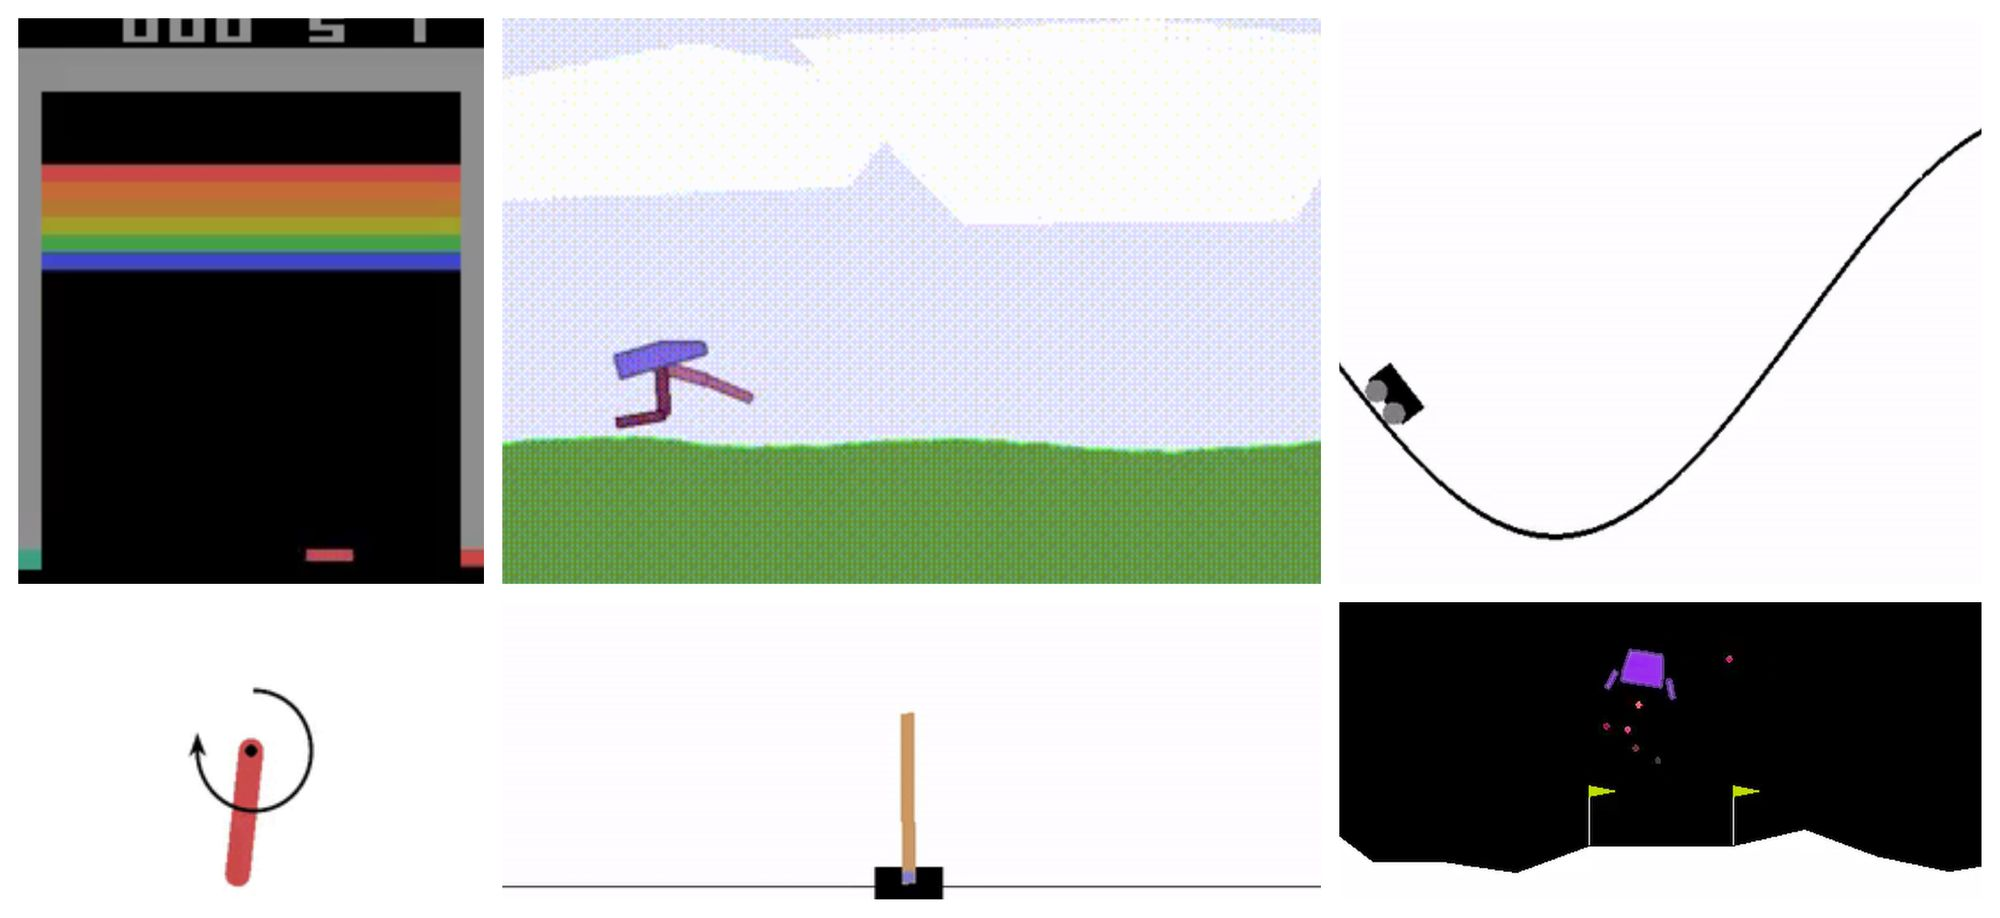
\includegraphics[width=15.0cm, height=7.5cm]{openaigym.jpg}
    \caption{Some of the OpenAI gym environments [99]}
\end{figure}

\subsection{Keras}
Keras is a high-level library built on TensorFlow. Developers can use Keras to build neural networks about mathematical aspects of tensor algebra, numerical techniques, and optimization methods [100].
\\ \\
The basic idea behind the development of Keras is to facilitate experiments with rapid prototyping. The ability to get from an idea to a conclusion with as little delay as possible is the cornerstone of good research. Keras is a library that stands out with its features in this sense.
\\ \\
This is a huge advantage for both academics and developers. Because they can dive directly into DL without going through too much trouble with low-level calculations. The increase in the demand for DL has led to an increase in the demand for knowledgeable people.
\\ \\
Many organizations tries to incorporate DL in some way. Keras basically helps you test and build DL applications with minimal effort. The API is intuitive enough to understand and very easy to use. During this project, version 2.8.0 for Keras library was used. 
%\begin{figure}[h]
%    \centering
%    
\includegraphics[width=11.0cm, height=6.0cm]{keras.jpg}
%    \caption{Logo of Keras and Tensorflow [100]}
%\end{figure}

\subsection{Pytorch}
Developed primarily by Meta AI, PyTorch is an open source optimized DL framework for tasks like computer vision and natural language using GPUs and CPUs. PyTorch is based on the Torch library. PyTorch features a C++ interface, even though the Python interface is more refined and the main focus of development [101]. 
\\ \\
Many DL applications have been developed on top of PyTorch, including Tesla Autopilot, Pyro from Uber, Transformers from Hugging Face, PyTorch Lightning, and Catalyst. 
\\ \\
The two key components of this library are tensor computing (similar to NumPy) with strong GPU acceleration and deep neural networks constructed using a tape-based automatic differentiation method.
%\begin{figure}[h]
%    \centering
%    
\includegraphics[width=11.0cm, height=6.0cm]{pytorch.jpeg}
%    \caption{Logo of Pytorch [101]}
%\end{figure}
\\ \\
During this project, version 1.8.1 for Pytorch library was used. Within the scope of this project, Keras was used as the main DL framework, but the same DL architecture was developed with Pytorch for the developers who will use and try to improve the output of this project. 

\subsection{Numpy}
A Python library for working with arrays is called NumPy. Additionally, it has the necessary operations for working with matrices, the Fourier transform, and linear algebra. In the year 2005, Travis Oliphant developed NumPy. You can use it for free because it is an open source project. Numerical Python is abbreviated as NumPy [102]. During this project, version 1.22.3 for NumPy library was used.
%\begin{figure}[h]
%    \centering
%    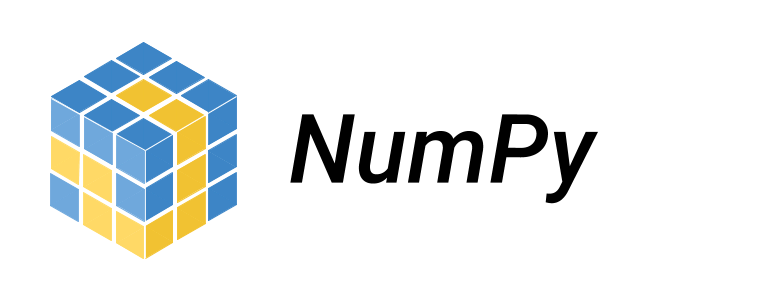
\includegraphics[width=10.0cm, height=5.0cm]{numpy.png}
%    \caption{Logo of NumPy [102]}
%\end{figure}

\subsection{Matplotlib}
The Matplotlib library is the most basic python library we use to visualize the data we have. It allows us to make 2D and 3D plots very easily. In this project, the robot's position, trajectory, movement and visualization of the robot itself were made with this library [103]. During this project, version 3.5.2 for Matplotlib library was used.
%\begin{figure}[h]
%    \centering
%    
\includegraphics[width=12.0cm, height=7.0cm]{matplotlib.png}
%    \caption{Logo of Matplotlib [103]}
%\end{figure}
%%%%%%%%%%%%%%%%%%%%%%%%%%%%%%%%%%%%%%%%%%%%%%%%%%%%%%%%%%%%%%%%%%%%%%%%%%%%%%%%%%%%%%%%%%%%%%%%%%%%%%%%%%%%%%%%%%%%%%%%%%%%%%%%%%%%%%%%%%%%%%%%%%%%%%%%%%%%%%%%%%%
%%%%%%%%%%%%%
%%%%%%%%%%%%%
%%%%%%%%%%%%%      MODEL OF THE ROBOT
%%%%%%%%%%%%%
%%%%%%%%%%%%%
%%%%%%%%%%%%%%%%%%%%%%%%%%%%%%%%%%%%%%%%%%%%%%%%%%%%%%%%%%%%%%%%%%%%%%%%%%%%%%%%%%%%%%%%%%%%%%%%%%%%%%%%%%%%%%%%%%%%%%%%%%%%%%%%%%%%%%%%%%%%%%%%%%%%%%%%%%%%%%%%%%%
\chapter{Kinematics Modelling of Continuum Robot}
Kinematics is a sub-branch of physics and is used to model many engineering problems. The science of kinematics deals with the motion of objects physically. In order to model engineering problems, it is generally accepted that the objects are solid (rigid), that is, that they do not change shape, that the object changes shape as a result of shear stresses applied to liquid particles. The science of kinematics is used to examine the position, velocity, acceleration and jerk values of solid and liquid objects according to the reference coordinate system they are connected to. While kinematics studies these properties of physical objects, it is not concerned with internal or external forces and moments that cause motion. The sub-branch of physics that studies the forces and moments that cause motion appears as the science of dynamics. Kinematics is used in the analysis of designed physical systems while solving engineering problems.
\\ \\
The science of kinematics is studied on subjects such as forward kinematics, inverse kinematics and velocity kinematics in robotic systems. In this thesis, forward and velocity kinematics calculations were made for continuum robots using the constant curvature method. The inverse kinematics of the continuum robot is not calculated. In this context, forwards kinematic analysis of continuum robot sections added one after another is concerned with the position and orientation of the robot's tip point in the task space, according to the translational or rotational motion of the end section points to which the robot's limbs are attached. Thus, depending on the change of the curvature variables of the robot, the position and orientation of the tip of the robot in task space changes. Inverse kinematics determines what the curvature variables of the robot should be in order for the robot to achieve the targeted position and orientation in the task space. This situation is seen in Figure 4.1.
\newpage
\begin{figure}[h]
    \centering
    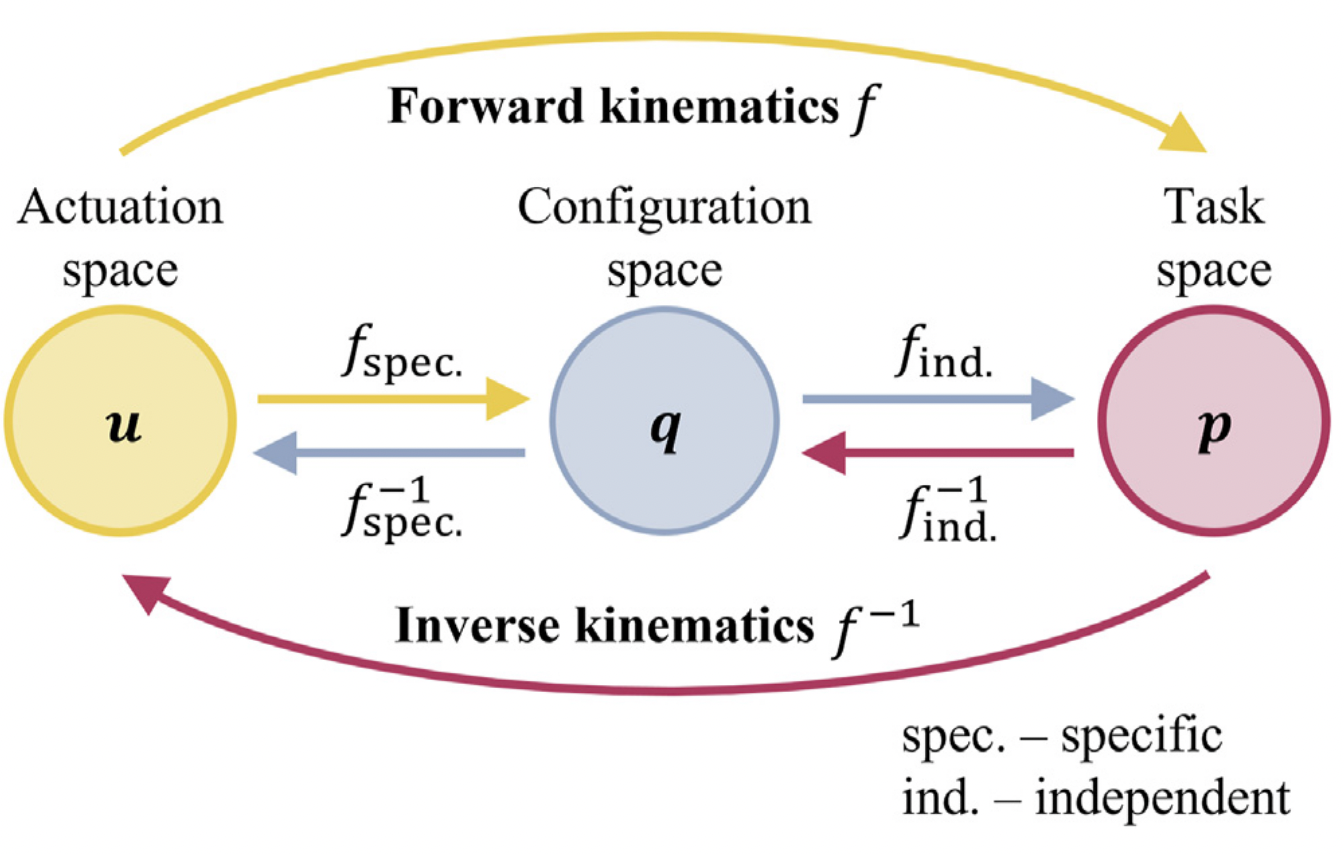
\includegraphics[width=13.4cm, height=8.5cm]{forward-inverse.png}
    \caption{Forward and inverse kinematics of continuum robot [5]}
\end{figure}

\noindent There are different methods in the literature for kinematic analysis of continuum robots. In the following subsection, Denavit Hartenberg (DH) method will be used for forward kinematic analysis of the robot. With this method, the forward kinematics problem of the robot is solved systematically. Geometric approaches are also available for forward kinematic solutions of robots. It should also be noted that various methods have been presented for modeling continuum robots [17]. In this thesis, we used the planar forward and velocity kinematics method presented by [36]. In order for the RL algorithm to be used in the project to be computationally cheaper, the model of the robot was designed as planar (2D) instead of spatial (3D).

\section{Forward Kinematics with D-H Method}
In this subsection, the geometric problem of a three section continuum robot and the forward kinematics problem with the DH method will be solved. This will provide an infrastructure for the RL approach, which is the model-free method proposed for the thesis.
\\ \\
We must first comprehend how to measure the motions of continuum designs. Due to the continuous nature of the design, unlike traditional manipulators, the use of joint angles and joint lengths does not provide a simple and physically feasible description of the shape of the manipulator. Instead, a kinematic model that describes the geometry of the manipulator using curvatures can offer a more real and understandable description of the manipulator.
\\ \\
Three coupled movements can be used to describe how a planar curve moves with constant curvature approach:
\begin{enumerate}
    \item rotation by an angle $\theta$
    \item translation by an amount of $\parallel x\parallel$, and
    \item rotation by the angle $\theta$ again,
\end{enumerate}
where x is defined to be the position vector of the endpoint of the curve.
\\ \\
We now have a discrete movement description of how the curve is moving. As would be done for conventional manipulators, we may now use a modified Denavit-Hartenberg (D-H) approach for the forward kinematic analysis. As a result, this strategy enables modeling continuum robots using a technique that is essentially acknowledged and utilized. The D-H process as modified is so-called because, contrary to the D-H procedure's premise that each joint should be independent from the others, in our situation the three motions are connected by the curvature. In reality, three basic, coupled motions are used to model a complex one DoF motion. The D-H table is as follows if the D-H frames for one section are configured as shown in Figure 4.2:
\begin{figure}[h]
    \centering
    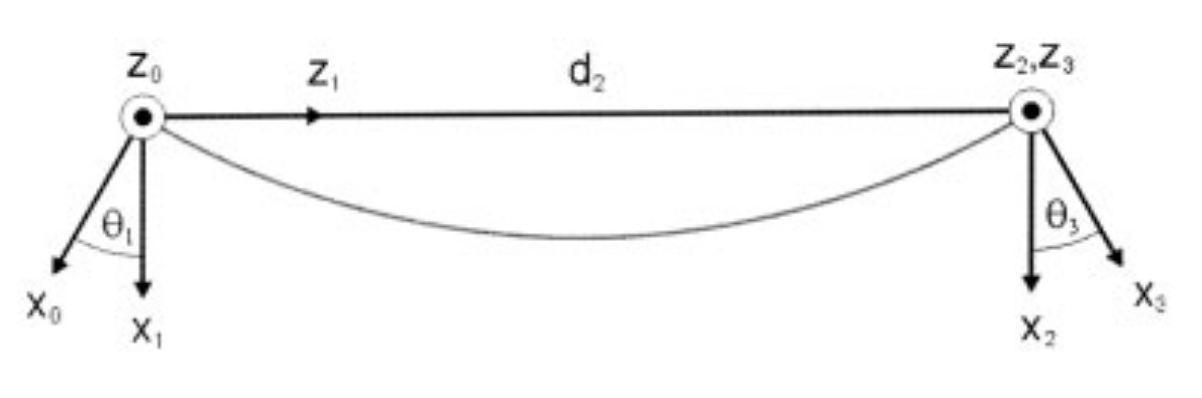
\includegraphics[width=12.0cm, height=4.0cm]{D-H.png}
    \caption{D-H frames for a planar section [36]}
\end{figure}
\newpage
Therefore, the D-H table is shown in Table 4.1.
\begin{table}[h!]
\centering
\begin{tabular}{rrrrr} 
\textbf{Link} & $\theta$ & $d$ & $a$ & $\alpha$ \\ [0.5ex] 
    \hline
    1 & $*$ & 0 & 0 & $-90^{\circ}$ \\
    2 & 0 & $*$ & 0 & $90^{\circ}$ \\
    3 & $*$ & 0 & 0 & $0^{\circ}$
\end{tabular}
\caption{D-H table of the Continuum Robot}
\end{table}

\noindent Using the above D-H table the homogeneous transformation matrix for the curve from frame 0 to frame 3 can be written in terms of the curvature $\kappa$ and the total arc length $l$ as
\begin{subequations}
\begin{align}
    A_{0}^{3}=A_{0}^{1}A_{1}^{2}A_{2}^{3}=\left[\begin{array}{cccc}
\cos (\kappa l) & -\sin (\kappa l) & 0 & \frac{\mathbf{1}}{\kappa}\{\cos (\kappa l)-1\} \\
\sin (\kappa l) & \cos (\kappa l) & 0 & \frac{\mathbf{1}}{\kappa} \sin (\kappa l) \\
0 & 0 & 1 & 0 \\
0 & 0 & 0 & 1
\end{array}\right]
\end{align}
\end{subequations}
The kinematic representation for a planar curve with constant curvature can now be derived using a method, and this method can be used to determine the kinematics of continuum robots. As discussed in section 3, most physically realizable continuum robots can be viewed as a combination of constant curvature sections. The forward kinematics of the robot can be obtained by the product of homogeneous transformation matrices as defined by equation 4.1. The inverse kinematics can then be determined using the Jacobian and the velocity kinematics as with conventional robots. To show this, an example using a three section planar continuum robot is presented.
\\ \\
The frames for a three section continuum robot can be setup as a combination of three sections, where each section's frames are shown in Figure 4.2. Using the simple and repetitive structure of the D-H table, the transformation matrix used for the forward kinematics is the product of three matrices of the form of equation 4.1. Therefore, the transformation matrix from frame 0 to frame 9 is shown in equation 4.2.
\begin{subequations}
\begin{align}
A_{0}^{9}= A_{0}^{3}A_{3}^{6}A_{6}^{9} = \left[\begin{array}{cccc}
\cos \left(\omega_{1}+\omega_{2}+\omega_{3}\right) & -\sin \left(\omega_{1}+\omega_{2}+\omega_{3}\right) & 0 & A_{14} \\
\sin \left(\omega_{1}+\omega_{2}+\omega_{3}\right) & \cos \left(\omega_{1}+\omega_{2}+\omega_{3}\right) & 0 & A_{24} \\
0 & 0 & 1 & 0 \\
0 & 0 & 0 & 1
\end{array}\right]
\end{align}
\end{subequations}
The previously undefined matrix elements are given as:
\begin{subequations}
\begin{align}
\begin{aligned}
A_{14}=& \frac{1}{\kappa_{1}}\left\{\cos \omega_{1}-1\right\}+\frac{1}{\kappa_{2}}\left\{\cos \left(\omega_{1}+\omega_{2}\right)-\cos \omega_{1}\right\} \\
&+\frac{1}{\kappa_{3}}\left\{\cos \left(\omega_{1}+\omega_{2}+\omega_{3}\right)-\cos \left(\omega_{1}+\omega_{2}\right)\right\} \\
A_{24}=& \frac{1}{\kappa_{1}} \sin \omega_{1}+\frac{1}{\kappa_{2}}\left\{\sin \left(\omega_{1}+\omega_{2}\right)-\sin \omega_{1}\right\} \\
&+\frac{1}{\kappa_{3}}\left\{\sin \left(\omega_{1}+\omega_{2}+\omega_{3}\right)-\sin \left(\omega_{1}+\omega_{2}\right)\right\}
\end{aligned}
\end{align}
\end{subequations}
where $\kappa_{i}$ and $l_{i}$ are the curvature and total arc length respectively for section $i$ and $\omega_{i}=\kappa_{i} l_{i}$ for $i=\{1,2,3\}$. Note, the total arc length for $i=\{1,2\}$ must be used so that section 3 is properly oriented, but any arc length can be used for the final section depending on where the point of interest lies in the section. The total arc length for the final section gives the kinematics in terms of the end point.
\\ \\
In Figure 4.3, you can see the simulated forward kinematics model of our robot with $\kappa_1 = 1.7035 [\frac{1}{m}]$, $\kappa_2 = 1.0 [\frac{1}{m}$], and $\kappa_3 = 2.0 [\frac{1}{m}]$ as curvature values of each section and $l_1 = 0.1 [m]$, $l_2 = 0.1 [m]$, and $l_3 = 0.1 [m]$ as length of each section. 
\newpage
\begin{figure}[h]
    \centering
    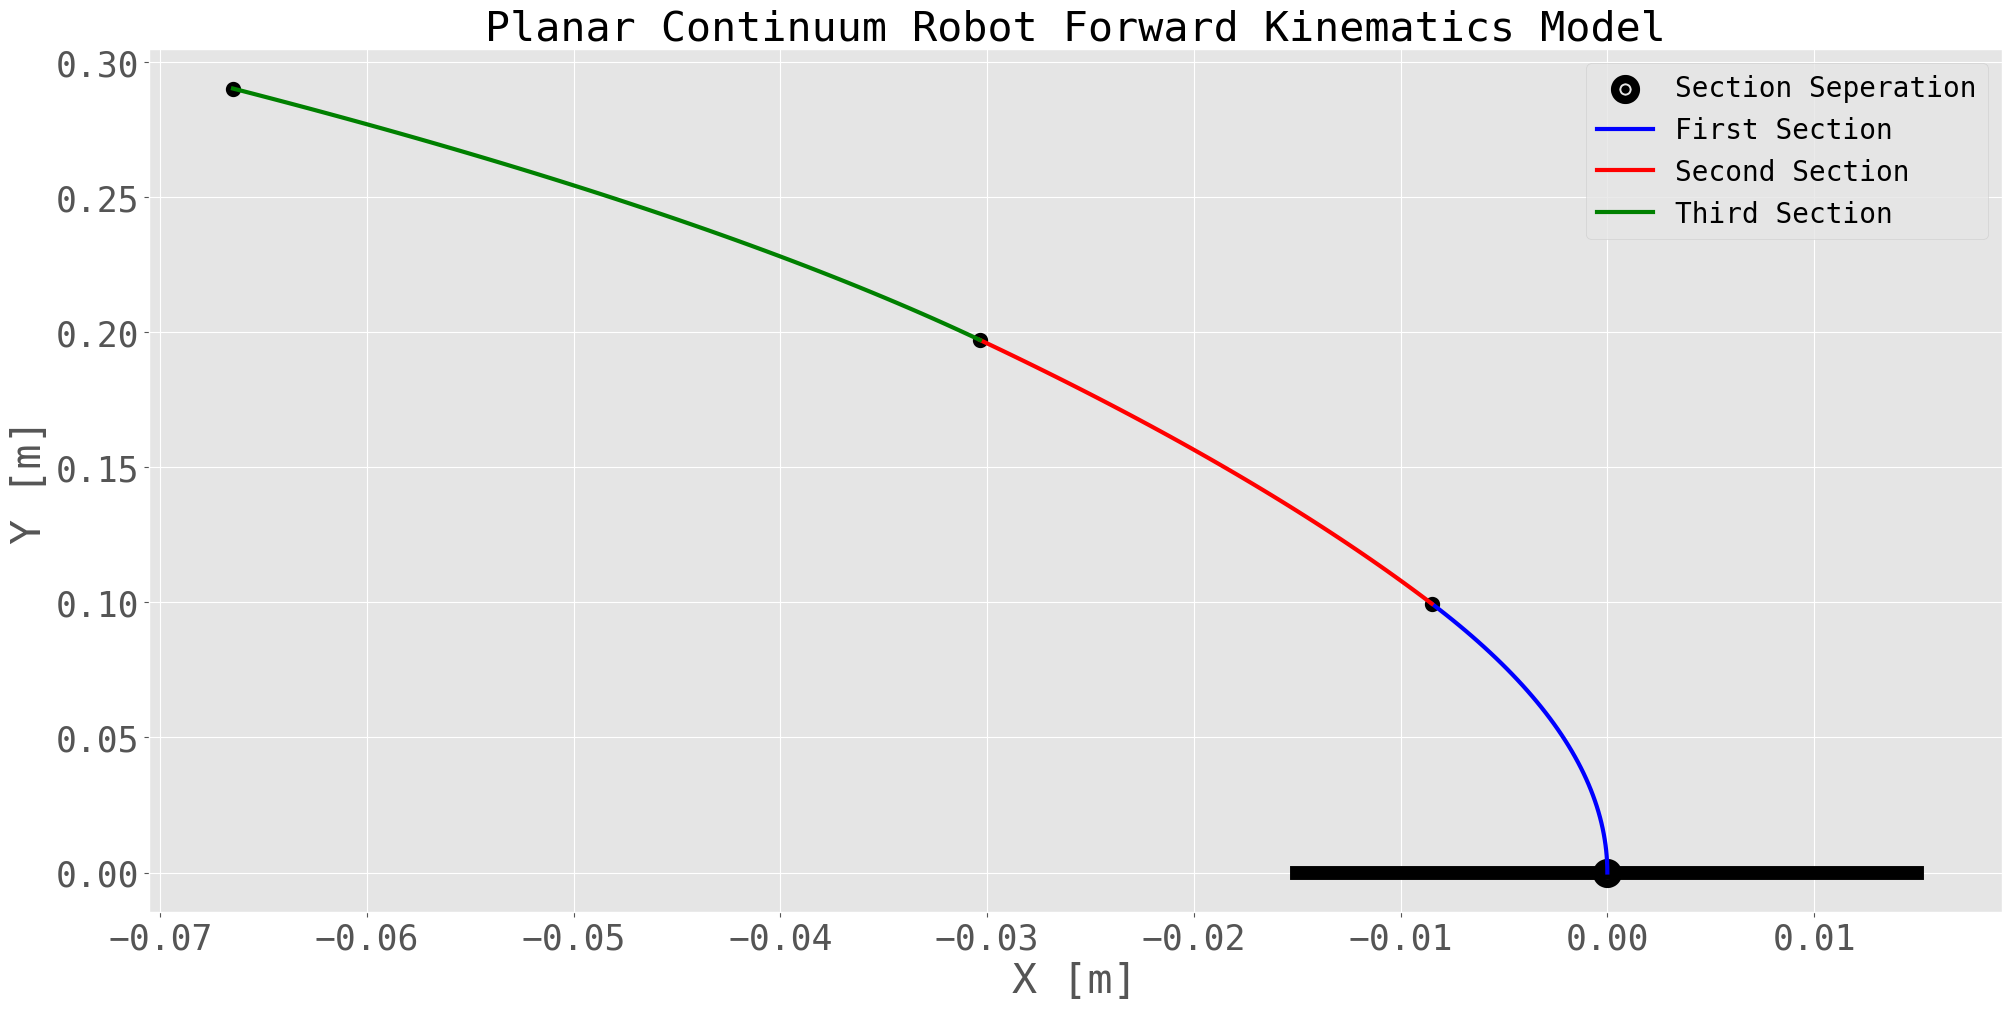
\includegraphics[width=16.0cm, height=8cm]{forward.png}
    \caption{Simulation result of forward kinematics}
\end{figure}

\section{Velocity Kinematics}
Analogous to conventional kinematic analysis [37] the velocity kinematics of a continuum robot can be written as
\begin{subequations}
\begin{align}
    \dot{x} = J\dot{q},
\end{align}
\end{subequations}
where $x\in \mathbb{R}^{m\times 1}$ is the task space vector, i.e., position and/or orientation, and the dot implies differentiation with respect to time. For our three section planar robot
\begin{subequations}
\begin{align}
    \mathbf{q} = \left [ \kappa _1, \kappa _2, \kappa _3 \right ]^T, \\
    \mathbf{\dot{q}} = \left [ \dot{\kappa _1}, \dot{\kappa _2}, \dot{\kappa _3} \right ]^T, \\
    \mathbf{\dot{x}} = \left [ \dot{x}, \dot{y} \right ]^T
\end{align}
\end{subequations}
The matrix $J$ is the Jacobian, and is a function of the 'joint' variables $\mathbf{q}$.
\\ \\
The elements of the Jacobian $J_{ij}$ can be obtained by partial derivatives of the forward kinematic equations as in 4.6:
\begin{subequations}
\begin{align}
    \begin{bmatrix}
\dot{x}\\ 
\dot{y}
\end{bmatrix} = \begin{bmatrix}
J_{11} & J_{12} \\ 
J_{21} & J_{22}
\end{bmatrix} \begin{bmatrix}
\dot{q_1}\\ 
\dot{q_2}
\end{bmatrix},
\end{align}
\end{subequations}
If we write it with chains rule, we will obtain equation 4.7.
\begin{subequations}
\begin{align}
\frac{dx}{dt} = \frac{\partial x}{\partial q_1} \frac{d q_1}{dt} + \frac{\partial x}{\partial q_2} \frac{d q_2}{dt}, \\ 
\frac{dy}{dt} = \frac{\partial y}{\partial q_1} \frac{d q_1}{dt} + \frac{\partial y}{\partial q_2} \frac{d q_2}{dt}
\end{align}
\end{subequations}
Let's apply this to our case as shown in equation 4.8.
\begin{subequations}
\begin{align}
    \frac{dx}{dt} = {\color{red} \frac{\partial x}{\partial \kappa_1}} \frac{d \kappa_1}{dt} + {\color{red} \frac{\partial x}{\partial \kappa_2} }\frac{d\kappa_2}{dt} +{\color{red}  \frac{\partial x}{\partial \kappa_3}} \frac{d \kappa_3}{dt}, \\
    \frac{dy}{dt} ={\color{red}  \frac{\partial y}{\partial \kappa_1}} \frac{d \kappa_1}{dt} + {\color{red} \frac{\partial y}{\partial \kappa_2}} \frac{d \kappa_2}{dt} + {\color{red} \frac{\partial y}{\partial \kappa_3}} \frac{d \kappa_3}{dt}
\end{align}
\end{subequations}
Red ones in equation 4.8 are the elements of our Jacobian Matrix. Let's define the Jacobian Matrix in equation 4.9.
\begin{subequations}
\begin{align}
    J = 
\begin{bmatrix}
 \frac{\partial x}{\partial \kappa_1}& \frac{\partial x}{\partial \kappa_2} &  \frac{\partial x}{\partial \kappa_3}\\
\frac{\partial y}{\partial \kappa_1} & \frac{\partial y}{\partial \kappa_2} & \frac{\partial y}{\partial \kappa_3} \\
\end{bmatrix}
\end{align}
\end{subequations}
As a result, the final form of equation 4.4 is seen in equation 4.10.
\begin{subequations}
\begin{align}
    \begin{bmatrix}
\frac{dx}{dt} \\ \frac{dy}{dt}
\end{bmatrix} =\begin{bmatrix}
 \frac{\partial x}{\partial \kappa_1}& \frac{\partial x}{\partial \kappa_2} &  \frac{\partial x}{\partial \kappa_3}\\
\frac{\partial y}{\partial \kappa_1} & \frac{\partial y}{\partial \kappa_2} & \frac{\partial y}{\partial \kappa_3} \\
\end{bmatrix} \begin{bmatrix}
\frac{d \kappa_1}{dt} \\ \frac{d \kappa_2}{dt}
 \\ \frac{d \kappa_3}{dt}
\end{bmatrix}
\end{align}
\end{subequations}
Jacobian matrices are a very practical tool that are extensively used in robotics as well as control theory. A Jacobian essentially describes the dynamic relationship between two different representations of a system. This relationship in our case is derivative of position and derivative of curvature. In velocity kinematics, the target is to describe the motion of end-effector (Tip of the continuum robot in our case). This motion is highly constrained by curvatures, which means describing the states of motion at those curvatures is describing the motion of the end-effector.
\newpage
\begin{algorithm}
\caption{Describing a motion with velocity kinematics}
\begin{algorithmic}[1]
\State Choose starting $\kappa_1$, $\kappa_2$, $\kappa_3$ as curvatures for each section and define $l_1$, $l_2$, and $l_3$ as length of each section.
\State Calculate Jacobian Matrix
\State Choose curvature velocities,$\dot{\kappa}$, for each $\kappa$
\While{True}
\State Calculate $\dot{x}$
\State Move the tip of the robot with velocities from step 3. $\triangleright$ $x_{t+1} = x_t + \dot{x_t}\cdot dt$
\State Update the jacobian as it is a function of the curvature, which have now changed
\EndWhile
\end{algorithmic}
\end{algorithm}

\begin{figure}[h]
    \centering
    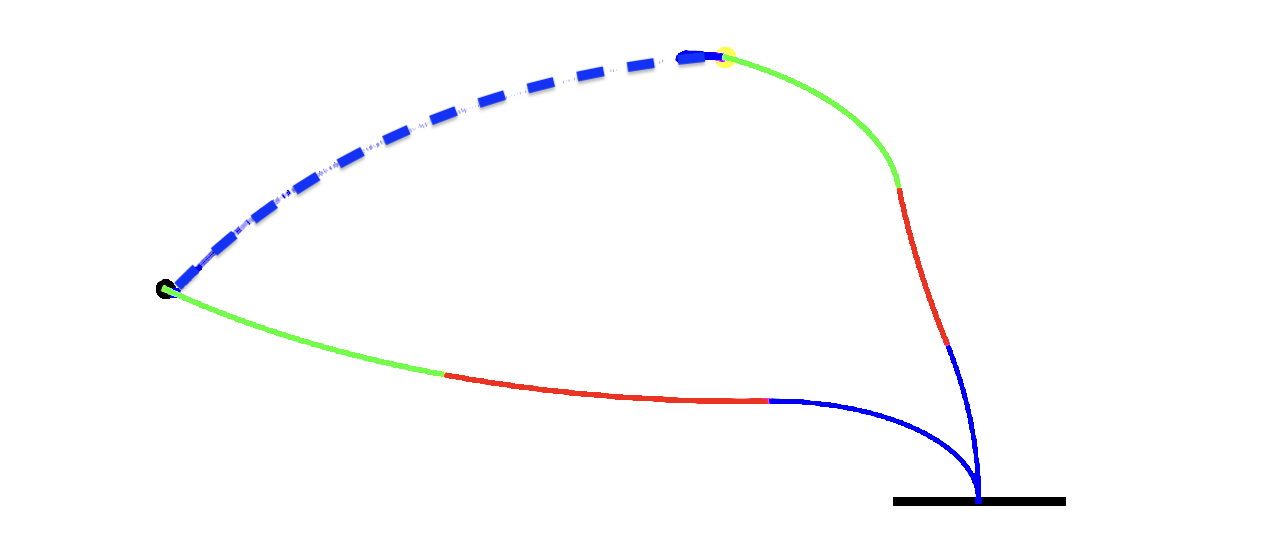
\includegraphics[width=16.0cm, height=8.0cm]{velocity_kin.png}
    \caption{Simulation result of velocity kinematics}
\end{figure}

\noindent In Figure 4.4, you can see the simulated velocity kinematics motion of our robot by applying Algorithm 4.8. Figure 4.4 shows only the motion of continuum robot's tip point. In this thesis, we used forward and velocity kinematics models while designing a RL environment for the continuum robot. In the next section, the details of the environment designed for RL will be discussed.
%%%%%%%%%%%%%%%%%%%%%%%%%%%%%%%%%%%%%%%%%%%%%%%%%%%%%%%%%%%%%%%%%%%%%%%%%%%%%%%%%%%%%%%%%%%%%%%%%%%%%%%%%%%%%%%%%%%%%%%%%%%%%%%%%%%%%%%%%%%%%%%%%%%%%%%%%%%%%%%%%%%
%%%%%%%%%%%%%
%%%%%%%%%%%%%
%%%%%%%%%%%%%      RL ENVIRONMENT
%%%%%%%%%%%%%
%%%%%%%%%%%%%
%%%%%%%%%%%%%%%%%%%%%%%%%%%%%%%%%%%%%%%%%%%%%%%%%%%%%%%%%%%%%%%%%%%%%%%%%%%%%%%%%%%%%%%%%%%%%%%%%%%%%%%%%%%%%%%%%%%%%%%%%%%%%%%%%%%%%%%%%%%%%%%%%%%%%%%%%%%%%%%%%%%
\chapter{Environment Design}
As mentioned in Section 3.4, a DDPG algorithm, which is a continuous RL control method, is used for continuum robot control within the scope of this thesis. A simple schematic diagram of this algorithm is shown in Figure 5.1. As can be seen in Figure 5.1, it is obvious that an environment is designed to control the robot through simulation. For this reason, in this part of the thesis, the details of the environment designed for the continuum robot simulation will be discussed.
\begin{figure}[h]
    \centering
    \includegraphics[width=11.7cm, height=9.3cm]{DDPG.png}
    \caption{Schematic diagram of Deep Deterministic Policy Gradient [38]}
\end{figure}

\noindent The diagram makes it clear how the environment, actors, and critics interact. After carrying out each action that the actor sent to the environment, the environment sent the critic an observation and a reward. Observation is nothing more than the environment's internal state. And the reward shows how effective the action was. Therefore, in order to use RL, we need two things:
\begin{itemize}
\item Actor and Critic Network: Simply two deep learning algorithms that determine the action to be given to the robot and the Q value.
\item Environment: A task or a simulation in which the robot's task space must be solved by the Actor-Critic.
\end{itemize}
As a result, an environment communicates with its agent (in this case, Actor-Critic) by providing its reward and state. The steps to creating an environment are listed below.
\begin{itemize}
\item Add a Action vector which represents the necessary action for agent to solve the environment.
\item Add a State vector which represents the internal state of the Simulation.
\item Add a meaningful Reward formulation into the Simulation so that agent can try to maximize or minimize it.
\end{itemize}

\noindent Our system's aim is to take the three segment continuum robot from a random starting point to a random target by using  the forward kinematics in (Equation 4.2) velocity kinematics formulas in (Equation 4.10) which are mentioned chapter 4.
\\ \\
The diagram below specifies the coordinate system used for the implementation of the continuum robot equations.
\begin{itemize}
    \item \textbf{$x-y$}: cartesian coordinates of the robot's tip point $m$. We don't have z axis since planar case for continuum robot was considered.
    \item \textbf{$\kappa$}: Curvatures  $\frac{1}{m}$.
    \item \textbf{$\dot{\kappa}$}: Derivative of curvatures $\frac{1}{\frac{m}{s}}$.
\end{itemize}
\newpage
\section{Action Space}
As mentioned earlier, action means that the artificial agent takes action by choosing from a separate list of possible actions. In this thesis, the action is a data structure of `ndarray` with shape `(3,)` representing the derivative of each segment's curvature. While the agent is moving in the created environment, it will produce 3 different curvature change rate values that are continuous in each step, and according to this rate of change, the robot must move and go towards the desired target. You can see the maximum and minimum values of the actions in Table 5.1. 
\begin{table}[h!]
\centering
\begin{tabular}{||c c c c||} 
 \hline \hline
 \textbf{Number} & \textbf{Action} & \textbf{Minimum} & \textbf{Maximum} \\ [0.5ex] 
    \hline\hline
    \multicolumn{1}{|l|}{0} & \multicolumn{1}{l|}{$\dot{\kappa_1}$} & \multicolumn{1}{l|}{-1.0} & \multicolumn{1}{l|}{1.0} \\ \hline
    \multicolumn{1}{|l|}{1} & \multicolumn{1}{l|}{$\dot{\kappa_2}$} & \multicolumn{1}{l|}{-1.0} & \multicolumn{1}{l|}{1.0} \\ \hline
    \multicolumn{1}{|l|}{2} & \multicolumn{1}{l|}{$\dot{\kappa_3}$} & \multicolumn{1}{l|}{-1.0} & \multicolumn{1}{l|}{1.0} \\ 
    \hline
\end{tabular}
\caption{Action Space Table}
\end{table}

\section{Observation Space}
The data our agent gathers from the environment is represented by observations or states. It may be a frame in the case of a video game (a screenshot). It might be the price of a specific stock, etc., in the case of the marketing agent. It's important to distinguish between observation and state: The world's current state can be fully described by the word "state" (there is no hidden information). in an area that is completely watched. The state can only be partially described by observation. in a setting that is only dimly observed.
\\ \\
As mentioned earlier, the state is a concrete and momentary state in which the agent finds himself; that is, a particular place and moment is an instant configuration that associates the agent with other important things such as vehicles, obstacles, enemies, or rewards. It can be the current state or any future state brought about by the environment. 
\\ \\
The state designed within the scope of the thesis is the instant x and y values of the robot in the cartesian system and the x and y values of the target point. You can see the maximum and minimum values of the actions in Table 5.2. The observation is a `ndarray` with shape `(4,)` representing the x-y coordinates of the robot's starting and end points. These values were obtained by a created task space calculation python script. The task space of the robot in the entire environment obtained by this script is shown in Figure 5.2. In this figure, you can see the task space of the robot with 180 sample of known curvatures and 30000 sample of unknown random curvatures. Under the each task space of the robot, you can see the distribution of the curvature values for each section. 
\begin{table}[h!]
\centering
\begin{tabular}{||c c c c||} 
 \hline \hline
 \textbf{Number} & \textbf{Observation} & \textbf{Minimum} & \textbf{Maximum} \\ [0.5ex] 
    \hline\hline
    \multicolumn{1}{|l|}{0} & \multicolumn{1}{l|}{$x$} & \multicolumn{1}{l|}{$-0.3$} & \multicolumn{1}{l|}{$0.2$} \\ \hline
    \multicolumn{1}{|l|}{1} & \multicolumn{1}{l|}{$y$} & \multicolumn{1}{l|}{$-0.15$} & \multicolumn{1}{l|}{$0.3$} \\ \hline
    \multicolumn{1}{|l|}{2} & \multicolumn{1}{l|}{$x_{goal}$} & \multicolumn{1}{l|}{$-0.27$} & \multicolumn{1}{l|}{$0.16$} \\ \hline
    \multicolumn{1}{|l|}{3} & \multicolumn{1}{l|}{$y_{goal}$} & \multicolumn{1}{l|}{$-0.11$} & \multicolumn{1}{l|}{$0.3$} \\ \hline
\end{tabular}
\caption{Observation Space Table}
\end{table}

\begin{figure}[h]
    \centering
    \includegraphics[width=16.0cm, height=8.0cm]{task_space_2.png}
    \caption{Simulation result of task space as well as the curvature values}
\end{figure}

\section{Rewards}
As mentioned earlier, it is the feedback by which the success or failure of an agent's actions in a given state is measured. Rewards can be immediate or delayed. They effectively evaluate the action of the agent. Let's define a distance metrics for error as shown in equation 5.1. This is a distance between position of the tip of continuum robot and the target point.
\begin{subequations}
\begin{align}
d_u = \sqrt{(x-x_{goal})^2+(y-y_{goal})^2}
\end{align}
\end{subequations}
The reward function for this thesis is defined as in equation 5.2.
\begin{subequations}
\begin{align}
r = -1\cdot (d_u)^{2} = -1\cdot(e)^{2}
\end{align}
\end{subequations}
which means that the reward is negative of the squared distance between the robot's tip point and the target point.
\\ \\
\noindent Other reward formulas were also developed within the scope of this thesis, but they were not used in the simulation. Testing of these rewards will be done in later stages. See equation 5.3 as an example of some other alternatives. 
\begin{subequations}
\begin{align}
r = d_{u-1} - d_{u}, \\ 
\medskip
r =\left\{\begin{array}{cc}
+1 & d_{u}<d_{u-1} \\
-1 & d_{u}>d_{u-1}
\end{array}\right.
\end{align}
\end{subequations}

%%%%%%%%%%%%%%%%%%%%%%%%%%%%%%%%%%%%%%%%%%%%%%%%%%%%%%%%%%%%%%%%%%%%%%%%%%%%%%%%%%%%%%%%%%%%%%%%%%%%%%%%%%%%%%%%%%%%%%%%%%%%%%%%%%%%%%%%%%%%%%%%%%%%%%%%%%%%%%%%%%%
%%%%%%%%%%%%%
%%%%%%%%%%%%%
%%%%%%%%%%%%%      SIMULATION
%%%%%%%%%%%%%
%%%%%%%%%%%%%
%%%%%%%%%%%%%%%%%%%%%%%%%%%%%%%%%%%%%%%%%%%%%%%%%%%%%%%%%%%%%%%%%%%%%%%%%%%%%%%%%%%%%%%%%%%%%%%%%%%%%%%%%%%%%%%%%%%%%%%%%%%%%%%%%%%%%%%%%%%%%%%%%%%%%%%%%%%%%%%%%%%
\chapter{Simulations and Results}
In this thesis, the control of the continuum robot was made with the DDPG algorithm, which is one of the continuous action methods of deep RL. The control scheme of the robot can bee seen in Figure 6.1. According to this scheme, a policy network called actor network uses as input the instantaneous position and the goal position in order to generate $\dot{\kappa}$ for each section. For a robot with three section we have input for the Policy network of size [4x1] and output $\dot{\kappa}$ of size [3x1] at each time step.
\begin{figure}[h]
    \centering
    \includegraphics[width=14.0cm, height=7.0cm]{control_scheme.png}
    \caption{General control scheme}
\end{figure}

\noindent The environment design required for the RL algorithm of the continuum robot to work is examined in detail in Chapter 5. Solving the continuum robot control problem with the DDPG algorithm is the basis for high-degree-of-freedom physical systems. Thanks to the Python software developed for the DDPG algorithm, the continuum manipulator provides the intended control and performs the movement from a random starting point to a random target point. Figure 6.2 shows the environment in which the robot is located and a random initial state.
\newpage
\begin{figure}[h]
    \centering
    \includegraphics[width=16cm, height=8cm]{initial_sim.png}
    \caption{One of the Robot's starting moments}
\end{figure}

\noindent In order for the continuum robot manipulative to perform learning with the DDPG algorithm, it needs to perform calculations iteratively in the simulation. Since learning through a physical robot will be very costly and time consuming, it is necessary to create a physical copy of the robot in the simulation environment. In this thesis, the kinematic equations of the robot were created in the simulation environment. The kinematic equations of the robot are expressed in Chapter 4.
\\ \\
In Chapter 3, the DDPG algorithm is discussed in detail. For this reason, no additional information will be given here. In order for this algorithm to work, various hyper-parameters must be entered. The values of hyper-parameters that give successful results in continuous robot control are given in Table 6.1. Firstly, the robot was trained with these hyper-parameters using both the Keras and Pytorch frameworks.
\newpage
\begin{table}[h!]
\centering
\begin{tabular}{||c c||} 
 \hline
 \textbf{Parameter} & \textbf{Value} \\ [0.5ex] 
    \hline\hline
    \multicolumn{1}{|l|}{Optimizer} & \multicolumn{1}{l|}{Adam} \\ \hline
    \multicolumn{1}{|l|}{Learning Rare Actor} & \multicolumn{1}{l|}{0.0001} \\ \hline
    \multicolumn{1}{|l|}{Learning Rate Critic} & \multicolumn{1}{l|}{0.0003} \\ \hline
    \multicolumn{1}{|l|}{Discount Factor $(\gamma)$} & \multicolumn{1}{l|}{0.99} \\ \hline
    \multicolumn{1}{|l|}{Batch Size} & \multicolumn{1}{l|}{128} \\ \hline
    \multicolumn{1}{|l|}{Replay Buffer Size} & \multicolumn{1}{l|}{1000000} \\ \hline
    \multicolumn{1}{|l|}{Actor Hidden Layer Number} & \multicolumn{1}{l|}{4} \\ \hline
    \multicolumn{1}{|l|}{Actor Hidden Layer Activation Function} & \multicolumn{1}{l|}{Relu} \\ \hline
    \multicolumn{1}{|l|}{Actor Output Layer Activation Function} & \multicolumn{1}{l|}{Tangent Hyperbolic} \\ \hline
    \multicolumn{1}{|l|}{Critic Hidden Layer Number} & \multicolumn{1}{l|}{4} \\ \hline
    \multicolumn{1}{|l|}{Critic Hidden Layer Activation Function} & \multicolumn{1}{l|}{Relu} \\ \hline
    \multicolumn{1}{|l|}{Critic Output Layer Activation Function} & \multicolumn{1}{l|}{Linear} \\ \hline
    \multicolumn{1}{|l|}{Maximum training steps} & \multicolumn{1}{l|}{1000} \\ \hline
    \multicolumn{1}{|l|}{Soft Update $(\tau)$} & \multicolumn{1}{l|}{0.001} \\ \hline
\end{tabular}
\caption{Hyper-parameters of DDPG Algorithm}
\end{table}

\noindent Also the DL architecture for the actor and critic is shown in Figure 6.3. Thanks to this figure you can see how many neuron for each hidden layer is used.
\newpage
\begin{figure}[h]
    \centering
    \includegraphics[width=16cm, height=8cm]{actor.png}
    \includegraphics[width=16cm, height=8cm]{critic.png}
    \caption{Actor-Critic architecture for DDPG algorithm}
\end{figure}

\noindent The difference between model parameters and model hyper-parameters must be understood. The configuration variables that are intrinsic to the model and whose values may be inferred from data are collectively referred to as the parameters (i.e. the weights of the neural networks). The learning process is assisted by the model hyper-parameters. They are manually specified before the training process begins, and as they have a significant impact on the model's performance, it is crucial to select the right values. The following provides descriptions of these hyper-parameters for the DDPG algorithm.
\begin{itemize}
    \item \textbf{Learning rate:} The learning rate regulates how quickly the model learns by dictating how much the model adjusts to the estimated error each time the weights are updated during training. If the value is too small, the training process could take a very long time, and if the learning rate is too high, the model might not converge.
    
    \item \textbf{Batch size:} This hyperparameter describes the number of tuples that are randomly selected during model training. A mini-batch gradient descent configuration is utilized (batch size is set to more than one but less than the total number of tuples).
    
    \item \textbf{Discount factor $(\gamma)$:} This hyperparameter is applied when moving on to the subsequent step. It establishes the relative weight that should be given to current and future rewards. While values close to 1 give more weight to future rewards, lower values emphasize current rewards.
    
    \item \textbf{Hidden layers:} They specify the neural network's size and number of layers. The more complex the problem, the more nodes and layers are required because they represent the ability to learn the best behavior. However, over-fitting will occur if the neural network is much larger than necessary.
    
    \item \textbf{Initial collect steps:} It indicates how many steps were completed prior to beginning the training with a random policy. In order to gather information about possible states that might not be reached during training, some data collection is done.
    
    \item \textbf{Maximum training steps:} It indicates the most iterations the simulation will go through. When analyzing the algorithm's convergence time, this hyper-parameter becomes less significant because the simulation typically ends before it reaches this value.
    
    \item \textbf{Soft Update $(\tau):$} With a soft update, we make little, periodic updates to the target network rather than all at once.
    
    \item \textbf{Optimizier:} Optimizers are techniques or strategies used to reduce a loss function (error function) or increase production efficiency. Optimizers are mathematical operations that depend on the weights and biases, which are the model's learning parameters. Optimizers provide guidance on how to modify the neural network's weights and learning rate to minimize losses.
    
    \item \textbf{Replay Buffer Size:} By collecting data from environment agents and taking samples from a big replay memory buffer over a range of unrelated experiences, it enables the DDPG agent to learn offline. This makes for a much speedier and more efficient training procedure.
    
    \item \textbf{Activation Function:} We need an activation function to introduce nonlinear real-world properties to artificial neural networks. If the activation function is not applied, the output signal becomes a simple linear function. A neural network without activation function will behave like a linear regression with limited learning power. In essence, activation functions explain the process by which nodes in a network layer convert the weighted total of their inputs into outputs.
\end{itemize}
Artificial neural networks and other variables used in the algorithm were created using the Nvidia CUDA infrastructure. Thanks to the CUDA library, calculations are made faster on the computer's graphics card. The technical specifications of the computer used for the training of the algorithm are intel i7 6700HQ 2.60 Ghz processor, 16 GB ddr4 ram, Nvdia 950M graphics card. At least 3000 episodes are required for the algorithm to perform a successful training. Thus, as a calculation step, at the end of 3,000,000 steps, the robot performs a good learning on the targeted region in the workspace. With this computer and hardware used, the training took approximately 14 hours.
\\ \\
The state, action and rewards invested for the operation of the robot's RL algorithm are mentioned in detail in Chapter 5. In the proposed algorithm, since the target point of the robot is randomly generated in each section, the robot needs to generalize the task space thoroughly. Thus, the trained model can generalize better. In response to the random $\dot{\kappa}$ values generated in the algorithm, the robot receives random values in the workspace. Training scheme can be seen in Figure 6.4.
\begin{figure}[h]
    \centering
    \includegraphics[width=12cm, height=6cm]{ddpg-scheme.png}
    \caption{Deep Deterministic Policy Gradient Training Scheme [105]}
\end{figure}

\noindent As mentioned above, the training took 14 hours and had a total of 3000 episodes. The 300-episodes moving averages of the rewards and each of the episodic reward received as a result of every episode were stored. The reason for using the 300-episode moving average is to see the plot more smoothly and interpret more effectively. The plot of these stored rewards are shown in Figure 6.5. In addition, both the average of the rewards and the rewards have been converted to log10 scale in the graph and are also shown in Figure 6.5.
\begin{figure}[h]
    \centering
    \includegraphics[width=16cm, height=8cm]{reward.png}
    \includegraphics[width=16cm, height=8cm]{rew_log.png}
    \caption{300-Episodes moving average of the rewards and each episodic reward per episode - per log10 of episode}
\end{figure}
\newpage
\noindent After the training is completed, a test script is written to test the algorithm. The test situations which contains any random test episode in which the robot is controlled are shown between Figure 6.6 and Figure 6.17. After the test script was written, 2 sample episodes were run and various plots will be shared below based on these two example of episodes. Firstly, you can see X-Axis, Y-Axis, and XY-Axis of the robot's trajectory in Figure 6.6, 6.7, and 6.8, respectively. It is clearly seen in these figures that after a while the trajectories converge to the desired reference trajectory with a small margin of error. These errors will be shown later.
\begin{figure}[h!]
    \centering
    \includegraphics[width=11cm, height=8cm]{traj_x_2.png}
    \includegraphics[width=11cm, height=8cm]{traj_x.png}
    \caption{Trajectory of robot in X-Axis for two different episodes}
\end{figure}
\newpage
\begin{figure}[h!]
    \centering
    \includegraphics[width=11cm, height=8cm]{traj_y_2.png}
    \includegraphics[width=11cm, height=8cm]{traj_y.png}
    \caption{Trajectory of robot in Y-Axis for two different episodes}
\end{figure}
\newpage
\begin{figure}[h!]
    \centering
    \includegraphics[width=11cm, height=8cm]{traj_x_y_2.png}
    \includegraphics[width=11cm, height=8cm]{traj_x_y.png}
    \caption{Trajectory of robot in XY-Axis for two different episodes}
\end{figure}

\noindent Then, the error values obtained as a result of these 2 episodes were stored and plotted. This plot is shown in Figure 6.9.
\newpage
\begin{figure}[h!]
    \centering
    \includegraphics[width=12.0cm, height=8.6cm]{error_test.png}
    \includegraphics[width=12.0cm, height=8.6cm]{error_test_2.png}
    \caption{Error of the robots position for two different episodes}
\end{figure}

\noindent Then, the error values for X-Axis, Y-Axis, and XY-Axis obtained as a result of these 2 episodes were stored and plotted. These plots are shown in Figures 6.10, 6.11, and 6.12.
\newpage
\begin{figure}[h!]
    \centering
    \includegraphics[width=11cm, height=8cm]{error_test_x.png}
    \includegraphics[width=11cm, height=8cm]{error_test_x_2.png}
    \caption{Error of robot in X-Axis for two different episodes}
\end{figure}
\newpage
\begin{figure}[h!]
    \centering
    \includegraphics[width=11cm, height=8cm]{error_test_y.png}
    \includegraphics[width=11cm, height=8cm]{error_test_y_2.png}
    \caption{Error of robot in Y-Axis for two different episodes}
\end{figure}
\newpage
\begin{figure}[h!]
    \centering
    \includegraphics[width=11cm, height=8cm]{error_test_x_y.png}
    \includegraphics[width=11cm, height=8cm]{error_test_x_y_2.png}
    \caption{Error of robot in XY-Axis for two different episodes}
\end{figure}

\noindent Finally, the change of the curvature values in time required to obtain these trajectories as a result of the two episodes are shown in Figure 6.13.
\newpage
\begin{figure}[h!]
    \centering
    \includegraphics[width=16cm, height=8cm]{curvature_values_2.png}
    \includegraphics[width=16cm, height=8cm]{curvature_values_3.png}
    \caption{Change of curvature values on each section for two different episodes}
\end{figure}

\noindent The simulation frame of one of the random episodes is given in Figure 6.14.
\newpage
\begin{figure}[h!]
    \centering
    \includegraphics[width=16cm, height=8cm]{target_arrived.png}
    \caption{Frame of an example successful episode.}
\end{figure}

\noindent After these samples were collected from two episodes, the robot was tested in 10 random episodes and the error values were stored as a result of these tests. The mean and standard deviation of the error values taken for these 10 different episodes were calculates and an error band graph was drawn. This graph is shown in Figures 6.15, and 6.16.
\begin{figure}[h!]
    \centering
    \includegraphics[width=15cm, height=7.5cm]{mean_err_x_y.png}
    \caption{Mean error of 10 episodes with error band}
\end{figure}
\newpage
\begin{figure}[h!]
    \centering
    \includegraphics[width=15cm, height=7.5cm]{mean_err_tot.png}
    \caption{Mean error of 10 episodes with error band in in XY-Axis}
\end{figure}
\noindent Based on the obtained results, the following conclusion was reached: as the robot learns at each step, the noise signal applied to the $\dot{\kappa}$ values decreases exponentially. This allows the robot to implement new movements based on its learned experiences, thereby affecting the trajectory it follows in task space. The DDPG algorithm for continuum robot control demonstrates increasingly successful results as training progresses. To improve the robot's performance with DDPG, it is possible to write reward functions that are appropriate for the robot. The reward function written for the robot should be created based on the actions that the robot must perform. In this thesis, the appropriate reward function is written to provide point-to-point access.
%%%%%%%%%%%%%%%%%%%%%%%%%%%%%%%%%%%%%%%%%%%%%%%%%%%%%%%%%%%%%%%%%%%%%%%%%%%%%%%%%%%%%%%%%%%%%%%%%%%%%%%%%%%%%%%%%%%%%%%%%%%%%%%%%%%%%%%%%%%%%%%%%%%%%%%%%%%%%%%%%%%
%%%%%%%%%%%%%
%%%%%%%%%%%%%
%%%%%%%%%%%%%      CONCLUSION
%%%%%%%%%%%%%
%%%%%%%%%%%%%
%%%%%%%%%%%%%%%%%%%%%%%%%%%%%%%%%%%%%%%%%%%%%%%%%%%%%%%%%%%%%%%%%%%%%%%%%%%%%%%%%%%%%%%%%%%%%%%%%%%%%%%%%%%%%%%%%%%%%%%%%%%%%%%%%%%%%%%%%%%%%%%%%%%%%%%%%%%%%%%%%%%

\chapter{Conclusions and Future Work}
This thesis proposes solving the continuum robot control problem using reinforcement learning (RL) algorithms. Chapter 3 discusses various alternative modeling and control methods for continuum robots, along with detailed discussions on the concepts of RL, deep RL, and deep learning (DL), and their application examples in the context of both continuum robots and RL.
\\ \\
Controlling robotic systems with a high degree of freedom (DoF) or unmodelable dynamics, particularly continuum systems with theoretically infinite DoF, presents significant challenges. However, the RL approach can address these control problems independently of the robot's mathematical model. Deep RL algorithms, in particular, offer a simpler solution for controlling high-DoF robots, redundant robots, and continuum robots. The advantage of RL over classical model-based approaches and optimal control methods lies in the fact that the reward function is tailored specifically for the problem at hand. In RL, the learning process occurs through states and the rewards generated from these states, making it a flexible and adaptive method for robotic control.
\\ \\
This thesis addresses the curvature control problem of a continuum robot as a low-level control issue in robotic systems, using the Deep Deterministic Policy Gradient (DDPG) algorithm. The DDPG algorithm is a model-free deep RL algorithm that provides continuous control, independent of the model. RL offers a superior approach to model-based control as it can perform the learning process independently of the physical system model. However, this thesis does not address high-level control issues in robotic systems, such as path planning in environments with obstacles.
\\ \\
The thesis yielded notable results in applying deep RL algorithms to continuum robot systems. The following areas may be considered for improvements or future research directions:
\begin{itemize}
    \item For high-level control, the problem of the robot creating path planning in environments with obstacles can be addressed using this algorithm.
    \item A moving target point can be designed and tracked.
    \item 3D position reaching problem can be solved.
    \item 3D position tracking problem can be solved.
    \item Different RL algorithms, such as Trust Region Policy Optimization (TRPO) or Proximal Policy Optimization (PPO) can be tested.
    \item  A real continuum robot can be constructed, and the same algorithm can be tested on this robot.
\end{itemize}

%%%%%%%%%%%%%%%%%%%%%%%%%%%%%%%%%%%%%%%%%%%%%%%%%%%%%%%%%%%%%%%%%%%%%%%%%%%%%%%%%%%%%%%%%%%%%%%%%%%%%%%%%%%%%%%%%%%%%%%%%%%%%%%%%%%%%%%%%%%%%%%%%%%%%%%%%%%%%%%%%%%
%%%%%%%%%%%%%
%%%%%%%%%%%%%
%%%%%%%%%%%%%      REFERENCES
%%%%%%%%%%%%%
%%%%%%%%%%%%%
%%%%%%%%%%%%%%%%%%%%%%%%%%%%%%%%%%%%%%%%%%%%%%%%%%%%%%%%%%%%%%%%%%%%%%%%%%%%%%%%%%%%%%%%%%%%%%%%%%%%%%%%%%%%%%%%%%%%%%%%%%%%%%%%%%%%%%%%%%%%%%%%%%%%%%%%%%%%%%%%%%%
\begin{thebibliography}{9}
\bibitem{1} Webster, R. J., and Jones, B. A. (2010). Design and Kinematic Modeling of Constant Curvature Continuum Robots: a Review. Int. J. Robotics Res. 29 (13), 1661 - 1683. doi:10.1177/0278364910368147
\bibitem{2} Robinson, G., and Davies, J. B. C. (1999). Continuum Robots-A State of the Art, in Proceedings 1999 IEEE international conference on robotics and automation (Cat. No. 99CH36288C), Detroit, MI, USA, May 10 - 15, 1999, 2849 - 2854.
\bibitem{3} Jones, B. A., and Walker, I. D. (2006). Practical Kinematics for Real-Time Implementation of Continuum Robots. IEEE Trans. Robot. 22 (6), 1087-1099. doi:10.1109/tro.2006.886268
\bibitem{4} Burgner-Kahrs, J., Rucker, D. C., and Choset, H. (2015). Continuum Robots for Medical Applications: A Survey. IEEE Trans. Robot. 31 (6), 1261-1280. doi:10.1109/tro.2015.2489500
\bibitem{5} X. Wang, Y. Li, and K. Kwok. A survey for machine learning-based control of continuum robots. Frontiers in Robotics and AI, 8:280, 2021. https://doi.org/10.3389/frobt.2021.730330
\bibitem{6} T. George Thuruthel, Y. Ansari, E. Falotico, C. Laschi, Control strategies for soft robotic manipulators: A survey. Soft Robot. 5, 149-163 (2018). https://doi.org/10.1089/soro.2017.0007
\bibitem{7} Trivedi, D., Rahn, C. D., Kier, W. M. Walker, I. D. Soft robotics: biological inspiration, state of the art, and future research. Appl. Bionics Biomech. 5, 99-117 (2008). DOI: 10.1080/11762320802557865
\bibitem{8} Pritts MB. 2005. Design and static analysis of a soft robotic manipulator [master's thesis]. University Park: The Pennsylvania State University.
\bibitem{9} I. D. Walker, Continuous backbone 'continuum' robot manipulators, ISRN Robotics, vol. 2013, Article ID 726506, 19 pages, 2013.
\bibitem{10} Kolachalama, S.; Lakshmanan, S.; Wang, W. Continuum Robots for Manipulation Applications: A Survey. J. Robot. 2020, 2020, 4187048.
\bibitem{11} G. Niu, J. Wang, and K. Xu, Model analysis for a continuum aircraft fuel tank inspection robot based on the Rzeppa universal joint, Advances in Mechanical Engineering, vol. 10, no. 5, 2018.
\bibitem{12} J. A. Engh, D. S. Minhas, D. Kondziolka, and C. N. Riviere, Percutaneous intracerebral navigation by duty-cycled spinning of flexible beveltipped needles. Neurosurgery, vol. 67, no. 4, pp. 1117-1122, 2010.
\bibitem{13} H. Stammberger and W. Posawetz, Functional endoscopic sinus surgery, Eur. Archives Oto-rhino-Laryngology, vol. 247, pp. 63-76, 1990.
\bibitem{14} N. Simaan, K. Xu, A. Kapoor, W. Wei, P. Kazanzides, P. Flint, and R. Taylor, Design and integration of a telerobotic system for minimally invasive surgery of the throat, Int. J. Robot. Res., vol. 28, no. 9, pp. 1134-1153, 2009.
\bibitem{15} L. H. Blumenschein, L. T. Gan, J. A. Fan, A. M. Okamura, and E. W. Hawkes, A tip-extending soft robot enables reconfigurable and deployable antennas, IEEE Robotics and Automation Letters, vol. 3, no. 2, pp. 949-956, 2018.
\bibitem{16} Godage, Isuru S.; Nanayakkara, Thrishantha; Caldwell, Darwin G. (October 2012). Locomotion with continuum limbs. 2012 IEEE/RSJ International Conference on Intelligent Robots and Systems. Vilamoura-Algarve, Portugal: IEEE: 293-298. doi:10.1109/IROS.2012.6385810.
\bibitem{17} P. Rao, Q. Peyron, S. Lilge, and J. Burgner-Kahrs, How to model tendon-driven continuum robots and benchmark modelling performance, Frontiers in Robotics and AI, vol. 7, p. 223, 2021.
\bibitem{18} Webster RJ, Jones BA. Design and Kinematic Modeling of Constant Curvature Continuum Robots: A Review. The International Journal of Robotics Research. 2010;29(13):1661-1683. doi:10.1177/0278364910368147
\bibitem{19} Sutton , Richard S. Barto, Andrew G., Reinforcement Learning An Introduction, Second Edition, London England: The MIT Press, (2018).
\bibitem{20} Team, K. (2020). Keras documentation: Deep Deterministic Policy Gradient (DDPG). Keras.io. https://keras.io/examples/rl/ddpg$\_$pendulum/
\bibitem{21} Introduction to Reinforcement Learning with David Silver. (2015). Deepmind.com.
\bibitem{22} Kolter, J. Zico., Introduction to Reinforcement Learning, Carnegie Mellon University, (2016).
\bibitem{23} Ogata, K. (2010). Modern control engineering (Vol. 5). Upper Saddle River, NJ: Prentice hall.
\bibitem{24} Garcia, Alberto Leon., Probability, Statistics, and Random Processes for Electrical Engineering, Third Edition, United States of America: Pearson Prentice Hall, (2005).
\bibitem{25} Kavukcuoglu, Koray., Mnih, Volodymyr., Silver, David., Human-level control through deep reinforcement learning, Nature, (2015)
\bibitem{26} Zhang, C.; Lu, Y. Study on artificial intelligence: The state of the art and future prospects. J. Ind. Inf. Integr. 2021, 23, 100224.
\bibitem{27} N. Buduma and N. Locascio, "Deep Learning", 2017
\bibitem{28} Abraham A (2005) Artificial Neural Networks. In: Peter H. Sydenham, Richard Thorn (ed) Handbook of measuring system design. John Wiley and Sons, London, pp 901-908
\bibitem{29} A. Jain, Fundamentals of deep learning. https://www.analyticsvidhya.com/blog/ 2016/03/introduction-deep-learning-fundamentals-neural-networks/, 2016. Accessed: 2017-06-16.
\bibitem{30} Activation Function - AI Wiki. (2022). Paperspace.com. https://machine-learning.paperspace.com/wiki/activation-function.
\bibitem{31} Introduction To Artificial Neural Networks. (2017). Vojtech.net. https://www.vojtech.net/posts/introduction-artificial-neural-networks
\bibitem{32} Educative Answers Team. (2020, January 17). Learning Rate in Machine learning. Educative: Interactive Courses for Software Developers; Educative. https://www.educative.io/answers/learning-rate-in-machine-learning
\bibitem{33} Amine ben khalifa, Hichem Frigui Multiple Instance Fuzzy Inference Neural Networks, 2016.
\bibitem{34} Mao, H., Alizadeh, M., Menache, I., and Kandula, S. (2016). Resource management with deep reinforcement learning. In ACM Workshop on Hot Topics in Networks (HotNets).
\bibitem{35} Lillicrap, Timothy P., Hunt, Jonathan J., Silver, David., Continuous Control With Deep Reinforcement Learning, International Conference on Learning Representations (ICLR), (2016).
\bibitem{36} Hannan, Walker, Kinematics and the Implementation of an Elephant's Trunk Manipulator and Other Continuum Style Robots (2003)
\bibitem{37} M. W. Spong and M. Vidyasagar, Robot dynamics and control, Wiley, New York, 1989.
\bibitem{38} Fan, L.; Zhang, J.; He, Y.; Liu, Y.; Hu, T.; Zhang, H. Optimal Scheduling of Microgrid Based on Deep Deterministic Policy Gradient and Transfer Learning. Energies 2021, 14, 584.
\bibitem{39} Moerland, T. M., Broekens, J., and Jonker, C. M. (2020). Model-Based Reinforcement Learning: A Survey. arXiv preprint arXiv:.16712.
\bibitem{40} Lee, K.-H., Fu, D. K. C., Leong, M. C. W., Chow, M., Fu, H.-C., Althoefer, K., et al. (2017a). Nonparametric Online Learning Control for Soft Continuum Robot: An Enabling Technique for Effective Endoscopic Navigation. Soft robotics 4 (4), 324-337. doi:10.1089/soro.2016.0065
\bibitem{41} Antman, S. S. (2005). Problems in Nonlinear Elasticity, in Nonlinear Problems of Elasticity New York City: Springer, 513-584.
\bibitem{42} Thuruthel, T. G., Falotico, E., Renda, F., and Laschi, C. (2018). Model-based Reinforcement Learning for Closed-Loop Dynamic Control of Soft Robotic Manipulators. IEEE Trans. Robotics 35 (1), 124-134. doi:10.1109/ TRO.2018.2878318
\bibitem{43} Wu, Q., Gu, Y., Li, Y., Zhang, B., Chepinskiy, S. A., Wang, J., et al. (2020). Position Control of Cable-Driven Robotic Soft Arm Based on Deep Reinforcement Learning. Information 11 (6), 310. doi:10.3390/info11060310
\bibitem{44} You,X.,Zhang,Y.,Chen,X.,Liu,X.,Wang,Z.,Jiang,H.,andChen,X.(2017). Modelfree Control for Soft Manipulators Based on Reinforcement Learning, in 2017 IEEE/RSJ International Conference on Intelligent Robots and Systems (IROS), Vancouver, Canada, Sep 24-28, 2017, 2909-2915. doi:10.1109/iros.2017.8206123
\bibitem{45} Satheeshbabu, S., Uppalapati, N. K., Chowdhary, G., and Krishnan, G. (2019). Open Loop Position Control of Soft Continuum Arm Using Deep Reinforcement Learning, in 2019 International Conference on Robotics and Automation (ICRA), Montreal, Canada, May 20-24, 2019, 5133-5139. doi:10.1109/icra.2019.8793653
\bibitem{46} You, H., Bae, E., Moon, Y., Kweon, J., and Choi, J. (2019). Automatic Control of Cardiac Ablation Catheter with Deep Reinforcement Learning Method. J. Mech. Sci. Technol. 33 (11), 5415-5423. doi:10.1007/s12206-019-1036-0
\bibitem{47} Ansari, Y., Manti, M., Falotico, E., Cianchetti, M., and Laschi, C. (2017). Multiobjective Optimization for Stiffness and Position Control in a Soft Robot Arm Module. IEEE Robotics Automation Lett. 3 (1), 108-115. doi:10.1109/LRA.2017.2734247
\bibitem{48} Satheeshbabu, S., Uppalapati, N. K., Fu, T., and Krishnan, G. (2020). Continuous Control of a Soft Continuum Arm Using Deep Reinforcement Learning, in 2020 3rd IEEE International Conference on Soft Robotics (RoboSoft), United States, May 15-July 15, 2020 (Yale University), 497-503.
\bibitem{49} Liu, X., Gasoto, R., Jiang, Z., Onal, C., and Fu, J. (2020). Learning to Locomote with Artificial Neural-Network and Cpg-Based Control in a Soft Snake Robot, in 2020 IEEE/RSJ International Conference on Intelligent Robots and Systems (IROS), Las Vegas, USA, Oct 25-29, 2020, 7758-7765. doi:10.1109/ iros45743.2020.9340763
\bibitem{50} Polydoros, A. S., and Nalpantidis, L. (2017). Survey of Model-Based Reinforcement Learning: Applications on Robotics. J. Intell. Robot Syst. 86 (2), 153-173. doi:10.1007/s10846-017-0468-y
\bibitem{51} Najar, A., and Chetouani, M. (2020). Reinforcement Learning with Human Advice. A Survey. arXiv preprint arXiv:.11016
\bibitem{52} Jiang, H., Wang, Z., Jin, Y., Chen, X., Li, P., Gan, Y., et al. (2021). Hierarchical Control of Soft Manipulators towards Unstructured Interactions. Int. J. Robotics Res. 40 (1), 411-434. doi:10.1177/0278364920979367
\bibitem{53} Gravagne I, Rahn C, Walker I. Large deflection dynamics and control for planar continuum robots. IEEE/ASME Trans Mechatron 2003;8:299-307.
\bibitem{54} Trivedi D, Lotfi A, Rahn C. Geometrically exact models for soft robotic manipulators. IEEE Trans Robot 2008;24: 773-780.
\bibitem{55} Jones B, Walker I. Kinematics for multisection continuum robots. IEEE Trans Robot 2006;22:43-55.
\bibitem{56} Bailly Y, Amirat Y. Modeling and control of a hybrid continuum active catheter for aortic aneurysm treatment. Proceedings of the 2005 IEEE International Conference on Robotics and Automation, Barcelona, Spain, 2005.
\bibitem{57} Camarillo D, Carlson C, Salisbury J. Configuration tracking for continuum manipulators with coupled tendon drive. IEEE Trans Robot 2009;25:798-808.
\bibitem{58} Camarillo DB, Carlson CR, Salisbury JK. Task-space control of continuum manipulators with coupled tendon drive. In: Experimental Robotics. Springer Tracts in Advanced Robotics, vol 54. Khatib O, Kumar V, Pappas GJ (Eds). Berlin, Heidelberg; Springer: 2009, pp. 271-280.
\bibitem{59} Xu K, Simaan N. Actuation compensation for flexible surgical snake-like robots with redundant remote actuation. Proceedings of the 2006 IEEE International Conference on Robotics and Automation (ICRA 2006), Orlando, FL, 2006.
\bibitem{60} Jones B, Walker I. Practical kinematics for real-time implementation of continuum robots. IEEE Trans Robot 2006; 22:1087-1099.
\bibitem{61} Bajo A, Goldman R, Simaan N. Configuration and joint feedback for enhanced performance of multi-segment continuum robots. 2011 IEEE International Conference on Robotics and Automation (ICRA), Shanghai, China, 2011.
\bibitem{62} Penning R, Jung J, Ferrier N, Zinn M. An evaluation of closedloop control options for continuum manipulators. 2012 IEEE International Conference on Robotics and Automation (ICRA), Saint Paul, MN, 2012.
\bibitem{63} Goldman R, Bajo A, Simaan N. Compliant motion control for continuum robots with intrinsic actuation sensing. 2011 IEEE International Conference on Robotics and Automation (ICRA), Shanghai, China, 2011.
\bibitem{64} Bajo A, Simaan N. Hybrid motion/force control of multibackbone continuum robots. Int J Robot Res 2015;35: 422-434.
\bibitem{65} Mahvash M, Dupont P. Stiffness control of surgical continuum manipulators. IEEE Trans Robot 2011;27:334-345. 
\bibitem{66} Wang H, Chen W, Yu X, Deng T, Wang X, Pfeifer R. Visual servo control of cable-driven soft robotic manipulator. 2013 IEEE/RSJ International Conference on Intelligent Robots and Systems (IROS), Tokyo, Japan, 2013. 
\bibitem{67} Mahl T, Hildebrandt A, Sawodny O. A variable curvature continuum kinematics for kinematic control of the bionic handling assistant. IEEE Trans Robot 2014;30:935-949.
\bibitem{68} Nguyen-Tuong D, Peters J. Model learning for robot control: a survey. Cogn Process 2011;12:319-340.
\bibitem{69} Giorelli M, Renda F, Ferri G, Laschi C. A feed-forward neural network learning the inverse kinetics of a soft cabledriven manipulator moving in three-dimensional space. 2013 IEEE/RSJ International Conference on Intelligent Robots and Systems (IROS), Tokyo, Japan, 2013.
\bibitem{70} Giorelli M, Renda F, Calisti M, Arienti A, Ferri G, Laschi C. Neural network and Jacobian method for solving the inverse statics of a cable-driven soft arm with nonconstant curvature. IEEE Trans Robot 2015;31:823-834.
\bibitem{71} Giorelli M, Renda F, Calisti M, Arienti A, Ferri G, Laschi C. Learning the inverse kinetics of an octopus-like manipulator in three-dimensional space. Bioinspir Biomim 2015; 10:035006.
\bibitem{72} Rolf M, Steil JJ. Efficient exploratory learning of inverse kinematics on a bionic elephant trunk. IEEE Trans Neural Netw Learn Syst 2014;25:1147-1160.
\bibitem{73} Yip M, Camarillo D. Model-less feedback control of continuum manipulators in constrained environments. IEEE Trans Robot 2014;30:880-889.
\bibitem{74} Malekzadeh M, Calinon S, Bruno D, Caldwell D. Learning by imitation with the STIFF-FLOP surgical robot: a biomimetic approach inspired by octopus movements. Robot Biomim 2014;1:13.
\bibitem{75} Ansari Y, Manti M, Falotico E, Cianchetti M, Laschi C. Multiobjective optimization for stiffness and position control in a soft robot arm module. IEEE Robot Autom Lett 2017;3:108-115.
\bibitem{76} Qi P, Liu C, Ataka A, Lam H, Althoefer K. Kinematic control of continuum manipulators using a fuzzy-model-based approach. IEEE Trans Industr Electron 2016;63:5022-5035.
\bibitem{77} Mnih, V., K. Kavukcuoglu, D. Silver, A. A. Rusu, J. Veness, M. G. Bellemare, A. Graves, M. Riedmiller, A. K. Fidjeland, G. Ostrovski, et al. 2015. Human-level control through deep reinforcement learning. Nature. 518(7540): 529-533.
\bibitem{78} Silver, D., A. Huang, C. J. Maddison, A. Guez, L. Sifre, G. Van Den Driessche, J. Schrittwieser, I. Antonoglou, V. Panneershelvam, M. Lanctot, et al. 2016b. Mastering the game of Go with deep neural networks and tree search. Nature. 529(7587): 484-489.
\bibitem{79} Brown, N. and T. Sandholm. 2017. Libratus: The Superhuman AI for No-Limit Poker. International Joint Conference on Artificial Intelligence (IJCAI-17).
\bibitem{80} Moravcik, M., M. Schmid, N. Burch, V. Lisy, D. Morrill, N. Bard, T. Davis, K. Waugh, M. Johanson, and M. Bowling. 2017. DeepStack: Expert-level artificial intelligence in heads-up no-limit poker. Science. 356(6337): 508-513.
\bibitem{81} Levine, S., C. Finn, T. Darrell, and P. Abbeel. 2016. End-to-end training of deep visuomotor policies. Journal of Machine Learning Research. 17(39): 1-40.
\bibitem{82} Gandhi, D., L. Pinto, and A. Gupta. 2017. Learning to Fly by Crashing. arXiv preprint arXiv:1704.05588
\bibitem{83} Pinto, L., M. Andrychowicz, P. Welinder, W. Zaremba, and P. Abbeel. 2017. Asymmetric Actor Critic for Image-Based Robot Learning. arXiv preprint arXiv:1710.06542.
\bibitem{84} You, Y., X. Pan, Z. Wang, and C. Lu. 2017. Virtual to Real Reinforcement Learning for Autonomous Driving. arXiv preprint arXiv:1704.03952.
\bibitem{85} Deng, Y., F. Bao, Y. Kong, Z. Ren, and Q. Dai. 2017. Deep direct reinforcement learning for financial signal representation and trading. IEEE transactions on neural networks and learning systems. 28(3): 653-664.
\bibitem{86} François-Lavet, V. 2017. Contributions to deep reinforcement learning and its applications in smartgrids. PhD thesis. University of Liege, Belgium.
\bibitem{87} T. Liu, Z. Tan, C. Xu, H. Chen, Z. Li, Study on deep reinforcement learning techniques for building energy consumption forecasting, Energy Build. 208 (2020) 109675, https://doi.org/10.1016/j.enbuild.2019.109675
\bibitem{88} OpenAI. (2021, June 18). OpenAI. OpenAI; OpenAI. https://openai.com/
\bibitem{89} OpenAI. (2019, December 13). OpenAI Five. OpenAI; OpenAI. https://openai.com/five/
\bibitem{90} Baker, B. (2019, September 17). Emergent Tool Use from Multi-Agent Interaction. OpenAI; OpenAI. https://openai.com/blog/emergent-tool-use/
\bibitem{91} OpenAI. (2019, October 15). Solving Rubik’s Cube with a Robot Hand. OpenAI; OpenAI. https://openai.com/blog/solving-rubiks-cube/
\bibitem{92} Palomeras N, El-Fakdi A, Carreras M, Ridao P (2012) Cola2: a control architecture for auvs. IEEE J Ocean Eng 37(4):695-716
\bibitem{93} Carlucho I, De Paula M, Wang S, Petillot Y, Acosta GG (2018) Adaptive low-level control of autonomous underwater vehicles using deep reinforcement learning. Robot Auton Syst 107:71-86
\bibitem{94} Faust A, Ruymgaart P, Salman M, Fierro R, Tapia L (2014) Continuous action reinforcement learning for control-affine systems with unknown dynamics. IEEE/CAA J Autom Sin 1(3):323-336
\bibitem{95} Wu C, Ju B, Wu Y, Lin X, Xiong N, Xu G, Li H, Liang X (2019) Uav autonomous target search based on deep reinforcement learning in complex disaster scene. IEEE Access 7:117227-117245
\bibitem{96} Wang Y, Lang H, De Silva CW (2010) A hybrid visual servo controller for robust grasping by wheeled mobile robots. IEEE/ASME Trans Mech 15(5):757-769
\bibitem{97} Adam S, Busoniu L, Babuska R (2011) Experience replay for real-time reinforcement learning control. IEEE Trans Syst Man Cybern Part C (Appl Rev) 42(2):201-212
\bibitem{98} Welcome to Python.org. (2022, August 8). Python.org; Python.org. https://www.python.org/
\bibitem{99} Gym Documentation. (2022). Gymlibrary.ml. https://www.gymlibrary.ml/
\bibitem{100} Team, K. (2022). Keras: the Python deep learning API. Keras.io. https://keras.io/
\bibitem{101} PyTorch. (2021). Pytorch.org. https://pytorch.org/
\bibitem{102} NumPy. (2022). Numpy.org. https://numpy.org/
\bibitem{103} Matplotlib - Visualization with Python. (2022). Matplotlib.org. https://matplotlib.org/
\bibitem{104} Mnih, Volodymyr, Kavukcuoglu, Koray, Silver, David, Graves, Alex, Antonoglou, Ioannis, Wierstra, Daan, and Riedmiller, Martin. Playing atari with deep reinforcement learning. arXiv preprint arXiv:1312.5602, 2013.
\bibitem{105} Deep Deterministic Policy Gradients. (2018). Github.io. https://deshpandeshrinath.github.io/blog/2018/05/05/DDPG
\bibitem{106} Buckingham, Rob; Graham, Andrew. Snake-Arm Robots - A New Tool for the Aerospace Industry. SAE Technical Paper Series. Warrendale, PA: SAE International. doi:10.4271/2003-01-2952.
\bibitem{107} Santiago, Jessie Lee C. Walker, Ian D. Godage, Isuru S. Continuum robots for space applications based on layer-jamming scales with stiffening capability doi:10.1109/aero.2015.7118897
\bibitem{108} Davies, J.B.C.; Lane, D.M.; Robinson, G.C.; O'Brien, D.J.; Pickett, M.; Sfakiotakis, M.; Deacon, B., Subsea applications of continuum robots, 363–369. doi:10.1109/UT.1998.670127.
\bibitem{109} Zheng, T., Branson, D. T., Kang, R., Cianchetti, M., Guglielmino, E., Follador, M., Caldwell, D. G. Dynamic continuum arm model for use with underwater robotic manipulators inspired by octopus vulgaris. doi:10.1109/icra.2012.6224685
\bibitem{110} Hinton, G. E., Osindero, S., Teh, Y. (2006). A fast learning algorithm for deep belief nets. Neural Computation, 18, 1527-1554.
\end{thebibliography}
\end{document}